
% \documentclass{article} % For LaTeX2e

% \usepackage{hyperref}
% \usepackage{url}
% \usepackage{microtype}
% \usepackage{graphicx} %[dvipdfmx]
% \usepackage{caption}
% \usepackage{subcaption}
% \usepackage{booktabs} 
% \usepackage{bbm}% for professional tables
% \usepackage{hyperref}
% \usepackage{tikz}
% \usepackage{wrapfig}
% \usepackage{amsmath}
% \usepackage{amssymb}
% \usepackage{mathtools}
% \usepackage{wrapfig}
% \usepackage{amsthm}
% \usepackage{float}

% \newcommand{\theHalgorithm}{\arabic{algorithm}}

% \usepackage[ruled, lined, linesnumbered, commentsnumbered, longend]{algorithm2e}

% \usepackage{xcolor}
% \definecolor{mygray}{gray}{0.4}

% %%%%% NEW MATH DEFINITIONS %%%%%

\usepackage{hyperref}
\usepackage{url}
\usepackage{microtype}
\usepackage{graphicx} %[dvipdfmx]
\usepackage{booktabs} 
\usepackage{multirow}

\usepackage{bbm}% for professional tables
\usepackage{hyperref}
\usepackage{tikz}
\usepackage{wrapfig}
\usepackage{amssymb}
\usepackage{mathtools}
\usepackage{wrapfig}
\usepackage{float}

\usepackage{amsmath,amsfonts,bm, amsthm}
\usepackage[ruled, lined, linesnumbered, commentsnumbered, longend]{algorithm2e}
\usepackage[normalem]{ulem}
\newcommand{\stkout}[1]{\ifmmode\text{\sout{\ensuremath{#1}}}\else\sout{#1}\fi}


\usepackage{microtype}
\usepackage{balance}
\usepackage{enumitem}
\usepackage{hyperref}
\usepackage{url}
\usepackage{bbold}
\newtheorem*{claim}{Claim} 
\usepackage[margin=1em]{caption}
\usepackage{subcaption}

\AtBeginDocument{%
%\setlength{\abovecaptionskip}{0pt}% if captions above content
\setlength{\belowcaptionskip}{12pt}% if captions below content
}

\newcommand{\M}[1]{{\mathbf{#1}}} % matrix
\newcommand{\T}[1]{{\mathcal{#1}}} % tensor
\newcommand{\V}[1]{{\mathbf{#1}}} % vector
\newcommand{\real}{{\mathbb{R}}} % real
\captionsetup{format=plain}



%%%%%%%%%%%%%%%%%%%%%%%%%%%%%%%%
% THEOREMS
%%%%%%%%%%%%%%%%%%%%%%%%%%%%%%%%
% \theoremstyle{plain}
% \newtheorem{theorem}{Theorem}[section]
% \newtheorem{proposition}[theorem]{Proposition}
% \newtheorem{lemma}[theorem]{Lemma}
% \newtheorem{corollary}[theorem]{Corollary}
% \theoremstyle{definition}
% \newtheorem{definition}[theorem]{Definition}
% \newtheorem{assumption}{Assumption}
% \newtheorem*{theorem*}{Theorem}


\theoremstyle{definition}
\newtheorem{theorem}{Theorem}
\newtheorem*{theorem*}{Theorem} %restate theorems
\newtheorem*{proposition*}{Proposition} %restate proposition
\newtheorem{lemma}{Lemma}
%\newtheorem{proposition}{Proposition}[theorem]
%eventually change to above version
\newtheorem{proposition}[theorem]{Proposition} 
\newtheorem{corollary}{Corollary}[theorem]
\newtheorem{definition}{Definition}[section]
\newtheorem{assumption}{Assumption}[section]
\newtheorem{notation}[theorem]{Notation}
\newtheorem{remark}{Remark}[theorem]



% \newtheorem{theorem}{Theorem}
\newtheorem*{prop*}{Proposition}
\newcommand{\rhoreg}{\rho_{\mathrm{reg}}}
\newcommand{\rhoin}{\rho_{\mathrm{in}}}
\newcommand{\rhoout}{\rho_{\mathrm{out}}}
\newcommand{\Rot}{\mathrm{Rot}}
\newcommand{\SOtwo}{\mathrm{SO}(2)}
\newcommand{\SO}{\mathrm{SO}}
\newcommand{\tout}{t_{\mathrm{out}}}
\newcommand{\tin}{t_{\mathrm{in}}}
\newcommand{\N}{[1\!\!:\!\!N]}



%\theoremstyle{plain}
% \newtheorem{theorem}{Theorem}[section]
% \newtheorem{proposition}[theorem]{Proposition}
% \newtheorem{lemma}[theorem]{Lemma}
% \newtheorem{corollary}[theorem]{Corollary}
% \newtheorem{assumption}{Assumption}
% \theoremstyle{definition}
% \newtheorem{definition}[theorem]{Definition}
% \theoremstyle{remark}
% \newtheorem{remark}[theorem]{Remark}

% Mark sections of captions for referring to divisions of figures
\newcommand{\figleft}{{\em (Left)}}
\newcommand{\figcenter}{{\em (Center)}}
\newcommand{\figright}{{\em (Right)}}
\newcommand{\figtop}{{\em (Top)}}
\newcommand{\figbottom}{{\em (Bottom)}}
\newcommand{\captiona}{{\em (a)}}
\newcommand{\captionb}{{\em (b)}}
\newcommand{\captionc}{{\em (c)}}
\newcommand{\captiond}{{\em (d)}}

% Highlight a newly defined term
\newcommand{\newterm}[1]{{\bf #1}}


% Figure reference, lower-case.
\def\figref#1{figure~\ref{#1}}
% Figure reference, capital. For start of sentence
\def\Figref#1{Figure~\ref{#1}}
\def\twofigref#1#2{figures \ref{#1} and \ref{#2}}
\def\quadfigref#1#2#3#4{figures \ref{#1}, \ref{#2}, \ref{#3} and \ref{#4}}
% Section reference, lower-case.
\def\secref#1{section~\ref{#1}}
% Section reference, capital.
\def\Secref#1{Section~\ref{#1}}
% Reference to two sections.
\def\twosecrefs#1#2{sections \ref{#1} and \ref{#2}}
% Reference to three sections.
\def\secrefs#1#2#3{sections \ref{#1}, \ref{#2} and \ref{#3}}
% Reference to an equation, lower-case.
\def\eqref#1{eqn~\ref{#1}}
% Reference to an equation, upper case
\def\Eqref#1{Eqn~\ref{#1}}
% A raw reference to an equation---avoid using if possible
\def\plaineqref#1{\ref{#1}}
% Reference to a chapter, lower-case.
\def\chapref#1{chapter~\ref{#1}}
% Reference to an equation, upper case.
\def\Chapref#1{Chapter~\ref{#1}}
% Reference to a range of chapters
\def\rangechapref#1#2{chapters\ref{#1}--\ref{#2}}
% Reference to an algorithm, lower-case.
\def\algref#1{algorithm~\ref{#1}}
% Reference to an algorithm, upper case.
\def\Algref#1{Algorithm~\ref{#1}}
\def\twoalgref#1#2{algorithms \ref{#1} and \ref{#2}}
\def\Twoalgref#1#2{Algorithms \ref{#1} and \ref{#2}}
% Reference to a part, lower case
\def\partref#1{part~\ref{#1}}
% Reference to a part, upper case
\def\Partref#1{Part~\ref{#1}}
\def\twopartref#1#2{parts \ref{#1} and \ref{#2}}

\def\ceil#1{\lceil #1 \rceil}
\def\floor#1{\lfloor #1 \rfloor}
\def\1{\bm{1}}
\newcommand{\train}{\mathcal{D}}
\newcommand{\valid}{\mathcal{D_{\mathrm{valid}}}}
\newcommand{\test}{\mathcal{D_{\mathrm{test}}}}

\def\eps{{\epsilon}}


% Random variables
\def\reta{{\textnormal{$\eta$}}}
\def\ra{{\textnormal{a}}}
\def\rb{{\textnormal{b}}}
\def\rc{{\textnormal{c}}}
\def\rd{{\textnormal{d}}}
\def\re{{\textnormal{e}}}
\def\rf{{\textnormal{f}}}
\def\rg{{\textnormal{g}}}
\def\rh{{\textnormal{h}}}
\def\ri{{\textnormal{i}}}
\def\rj{{\textnormal{j}}}
\def\rk{{\textnormal{k}}}
\def\rl{{\textnormal{l}}}
% rm is already a command, just don't name any random variables m
\def\rn{{\textnormal{n}}}
\def\ro{{\textnormal{o}}}
\def\rp{{\textnormal{p}}}
\def\rq{{\textnormal{q}}}
\def\rr{{\textnormal{r}}}
\def\rs{{\textnormal{s}}}
\def\rt{{\textnormal{t}}}
\def\ru{{\textnormal{u}}}
\def\rv{{\textnormal{v}}}
%\def\rw{{\textnormal{w}}}
\def\rx{{\textnormal{x}}}
%\def\ry{{\textnormal{y}}}
\newcommand{\ry}[1] {{\color{magenta} [RY: #1] } }
\newcommand{\edit}[1] { #1 } 
\newcommand{\sofi}[1] {{\color{blue} [sophia: #1] }}
\newcommand{\plusminus}[1] { \scriptsize{$\pm$ #1}}
\def\rz{{\textnormal{z}}}
% Random vectors
\def\rvepsilon{{\mathbf{\epsilon}}}
\def\rvtheta{{\mathbf{\theta}}}
\def\rva{{\mathbf{a}}}
\def\rvb{{\mathbf{b}}}
\def\rvc{{\mathbf{c}}}
\def\rvd{{\mathbf{d}}}
\def\rve{{\mathbf{e}}}
\def\rvf{{\mathbf{f}}}
\def\rvg{{\mathbf{g}}}
\def\rvh{{\mathbf{h}}}
\def\rvu{{\mathbf{i}}}
\def\rvj{{\mathbf{j}}}
\def\rvk{{\mathbf{k}}}
\def\rvl{{\mathbf{l}}}
\def\rvm{{\mathbf{m}}}
\def\rvn{{\mathbf{n}}}
\def\rvo{{\mathbf{o}}}
\def\rvp{{\mathbf{p}}}
\def\rvq{{\mathbf{q}}}
\def\rvr{{\mathbf{r}}}
\def\rvs{{\mathbf{s}}}
\def\rvt{{\mathbf{t}}}
\def\rvu{{\mathbf{u}}}
\def\rvv{{\mathbf{v}}}
\def\rvw{{\mathbf{w}}}
\def\rvx{{\mathbf{x}}}
\def\rvy{{\mathbf{y}}}
\def\rvz{{\mathbf{z}}}

% Elements of random vectors
\def\erva{{\textnormal{a}}}
\def\ervb{{\textnormal{b}}}
\def\ervc{{\textnormal{c}}}
\def\ervd{{\textnormal{d}}}
\def\erve{{\textnormal{e}}}
\def\ervf{{\textnormal{f}}}
\def\ervg{{\textnormal{g}}}
\def\ervh{{\textnormal{h}}}
\def\ervi{{\textnormal{i}}}
\def\ervj{{\textnormal{j}}}
\def\ervk{{\textnormal{k}}}
\def\ervl{{\textnormal{l}}}
\def\ervm{{\textnormal{m}}}
\def\ervn{{\textnormal{n}}}
\def\ervo{{\textnormal{o}}}
\def\ervp{{\textnormal{p}}}
\def\ervq{{\textnormal{q}}}
\def\ervr{{\textnormal{r}}}
\def\ervs{{\textnormal{s}}}
\def\ervt{{\textnormal{t}}}
\def\ervu{{\textnormal{u}}}
\def\ervv{{\textnormal{v}}}
\def\ervw{{\textnormal{w}}}
\def\ervx{{\textnormal{x}}}
\def\ervy{{\textnormal{y}}}
\def\ervz{{\textnormal{z}}}

% Random matrices
\def\rmA{{\mathbf{A}}}
\def\rmB{{\mathbf{B}}}
\def\rmC{{\mathbf{C}}}
\def\rmD{{\mathbf{D}}}
\def\rmE{{\mathbf{E}}}
\def\rmF{{\mathbf{F}}}
\def\rmG{{\mathbf{G}}}
\def\rmH{{\mathbf{H}}}
\def\rmI{{\mathbf{I}}}
\def\rmJ{{\mathbf{J}}}
\def\rmK{{\mathbf{K}}}
\def\rmL{{\mathbf{L}}}
\def\rmM{{\mathbf{M}}}
\def\rmN{{\mathbf{N}}}
\def\rmO{{\mathbf{O}}}
\def\rmP{{\mathbf{P}}}
\def\rmQ{{\mathbf{Q}}}
\def\rmR{{\mathbf{R}}}
\def\rmS{{\mathbf{S}}}
\def\rmT{{\mathbf{T}}}
\def\rmU{{\mathbf{U}}}
\def\rmV{{\mathbf{V}}}
\def\rmW{{\mathbf{W}}}
\def\rmX{{\mathbf{X}}}
\def\rmY{{\mathbf{Y}}}
\def\rmZ{{\mathbf{Z}}}

% Elements of random matrices
\def\ermA{{\textnormal{A}}}
\def\ermB{{\textnormal{B}}}
\def\ermC{{\textnormal{C}}}
\def\ermD{{\textnormal{D}}}
\def\ermE{{\textnormal{E}}}
\def\ermF{{\textnormal{F}}}
\def\ermG{{\textnormal{G}}}
\def\ermH{{\textnormal{H}}}
\def\ermI{{\textnormal{I}}}
\def\ermJ{{\textnormal{J}}}
\def\ermK{{\textnormal{K}}}
\def\ermL{{\textnormal{L}}}
\def\ermM{{\textnormal{M}}}
\def\ermN{{\textnormal{N}}}
\def\ermO{{\textnormal{O}}}
\def\ermP{{\textnormal{P}}}
\def\ermQ{{\textnormal{Q}}}
\def\ermR{{\textnormal{R}}}
\def\ermS{{\textnormal{S}}}
\def\ermT{{\textnormal{T}}}
\def\ermU{{\textnormal{U}}}
\def\ermV{{\textnormal{V}}}
\def\ermW{{\textnormal{W}}}
\def\ermX{{\textnormal{X}}}
\def\ermY{{\textnormal{Y}}}
\def\ermZ{{\textnormal{Z}}}

% Vectors
\def\vzero{{\bm{0}}}
\def\vone{{\bm{1}}}
\def\vmu{{\bm{\mu}}}
\def\vtheta{{\bm{\theta}}}
\def\va{{\bm{a}}}
\def\vb{{\bm{b}}}
\def\vc{{\bm{c}}}
\def\vd{{\bm{d}}}
\def\ve{{\bm{e}}}
\def\vf{{\bm{f}}}
\def\vg{{\bm{g}}}
\def\vh{{\bm{h}}}
\def\vi{{\bm{i}}}
\def\vj{{\bm{j}}}
\def\vk{{\bm{k}}}
\def\vl{{\bm{l}}}
\def\vm{{\bm{m}}}
\def\vn{{\bm{n}}}
\def\vo{{\bm{o}}}
\def\vp{{\bm{p}}}
\def\vq{{\bm{q}}}
\def\vr{{\bm{r}}}
\def\vs{{\bm{s}}}
\def\vt{{\bm{t}}}
\def\vu{{\bm{u}}}
\def\vv{{\bm{v}}}
\def\vw{{\bm{w}}}
\def\vx{{\bm{x}}}
\def\vy{{\bm{y}}}
\def\vz{{\bm{z}}}

% Elements of vectors
\def\evalpha{{\alpha}}
\def\evbeta{{\beta}}
\def\evepsilon{{\epsilon}}
\def\evlambda{{\lambda}}
\def\evomega{{\omega}}
\def\evmu{{\mu}}
\def\evpsi{{\psi}}
\def\evsigma{{\sigma}}
\def\evtheta{{\theta}}
\def\eva{{a}}
\def\evb{{b}}
\def\evc{{c}}
\def\evd{{d}}
\def\eve{{e}}
\def\evf{{f}}
\def\evg{{g}}
\def\evh{{h}}
\def\evi{{i}}
\def\evj{{j}}
\def\evk{{k}}
\def\evl{{l}}
\def\evm{{m}}
\def\evn{{n}}
\def\evo{{o}}
\def\evp{{p}}
\def\evq{{q}}
\def\evr{{r}}
\def\evs{{s}}
\def\evt{{t}}
\def\evu{{u}}
\def\evv{{v}}
\def\evw{{w}}
\def\evx{{x}}
\def\evy{{y}}
\def\evz{{z}}

% Matrix
\def\mA{{\bm{A}}}
\def\mB{{\bm{B}}}
\def\mC{{\bm{C}}}
\def\mD{{\bm{D}}}
\def\mE{{\bm{E}}}
\def\mF{{\bm{F}}}
\def\mG{{\bm{G}}}
\def\mH{{\bm{H}}}
\def\mI{{\bm{I}}}
\def\mJ{{\bm{J}}}
\def\mK{{\bm{K}}}
\def\mL{{\bm{L}}}
\def\mM{{\bm{M}}}
\def\mN{{\bm{N}}}
\def\mO{{\bm{O}}}
\def\mP{{\bm{P}}}
\def\mQ{{\bm{Q}}}
\def\mR{{\bm{R}}}
\def\mS{{\bm{S}}}
\def\mT{{\bm{T}}}
\def\mU{{\bm{U}}}
\def\mV{{\bm{V}}}
\def\mW{{\bm{W}}}
\def\mX{{\bm{X}}}
\def\mY{{\bm{Y}}}
\def\mZ{{\bm{Z}}}
\def\mBeta{{\bm{\beta}}}
\def\mPhi{{\bm{\Phi}}}
\def\mLambda{{\bm{\Lambda}}}
\def\mSigma{{\bm{\Sigma}}}

% Tensor
\DeclareMathAlphabet{\mathsfit}{\encodingdefault}{\sfdefault}{m}{sl}
\SetMathAlphabet{\mathsfit}{bold}{\encodingdefault}{\sfdefault}{bx}{n}
\newcommand{\tens}[1]{\bm{\mathsfit{#1}}}
\def\tA{{\tens{A}}}
\def\tB{{\tens{B}}}
\def\tC{{\tens{C}}}
\def\tD{{\tens{D}}}
\def\tE{{\tens{E}}}
\def\tF{{\tens{F}}}
\def\tG{{\tens{G}}}
\def\tH{{\tens{H}}}
\def\tI{{\tens{I}}}
\def\tJ{{\tens{J}}}
\def\tK{{\tens{K}}}
\def\tL{{\tens{L}}}
\def\tM{{\tens{M}}}
\def\tN{{\tens{N}}}
\def\tO{{\tens{O}}}
\def\tP{{\tens{P}}}
\def\tQ{{\tens{Q}}}
\def\tR{{\tens{R}}}
\def\tS{{\tens{S}}}
\def\tT{{\tens{T}}}
\def\tU{{\tens{U}}}
\def\tV{{\tens{V}}}
\def\tW{{\tens{W}}}
\def\tX{{\tens{X}}}
\def\tY{{\tens{Y}}}
\def\tZ{{\tens{Z}}}


% Graph
\def\gA{{\mathcal{A}}}
\def\gB{{\mathcal{B}}}
\def\gC{{\mathcal{C}}}
\def\gD{{\mathcal{D}}}
\def\gE{{\mathcal{E}}}
\def\gF{{\mathcal{F}}}
\def\gG{{\mathcal{G}}}
\def\gH{{\mathcal{H}}}
\def\gI{{\mathcal{I}}}
\def\gJ{{\mathcal{J}}}
\def\gK{{\mathcal{K}}}
\def\gL{{\mathcal{L}}}
\def\gM{{\mathcal{M}}}
\def\gN{{\mathcal{N}}}
\def\gO{{\mathcal{O}}}
\def\gP{{\mathcal{P}}}
\def\gQ{{\mathcal{Q}}}
\def\gR{{\mathcal{R}}}
\def\gS{{\mathcal{S}}}
\def\gT{{\mathcal{T}}}
\def\gU{{\mathcal{U}}}
\def\gV{{\mathcal{V}}}
\def\gW{{\mathcal{W}}}
\def\gX{{\mathcal{X}}}
\def\gY{{\mathcal{Y}}}
\def\gZ{{\mathcal{Z}}}

% Sets
\def\sA{{\mathbb{A}}}
\def\sB{{\mathbb{B}}}
\def\sC{{\mathbb{C}}}
\def\sD{{\mathbb{D}}}
% Don't use a set called E, because this would be the same as our symbol
% for expectation.
\def\sF{{\mathbb{F}}}
\def\sG{{\mathbb{G}}}
\def\sH{{\mathbb{H}}}
\def\sI{{\mathbb{I}}}
\def\sJ{{\mathbb{J}}}
\def\sK{{\mathbb{K}}}
\def\sL{{\mathbb{L}}}
\def\sM{{\mathbb{M}}}
\def\sN{{\mathbb{N}}}
\def\sO{{\mathbb{O}}}
\def\Prob{{\mathbb{P}}}
\def\prob{{\mathbb{P}}}
\def\sQ{{\mathbb{Q}}}
\def\sR{{\mathbb{R}}}
\def\sS{{\mathbb{S}}}
\def\sT{{\mathbb{T}}}
\def\sU{{\mathbb{U}}}
\def\sV{{\mathbb{V}}}
\def\sW{{\mathbb{W}}}
\def\sX{{\mathbb{X}}}
\def\sY{{\mathbb{Y}}}
\def\sZ{{\mathbb{Z}}}

% Entries of a matrix
\def\emLambda{{\Lambda}}
\def\emA{{A}}
\def\emB{{B}}
\def\emC{{C}}
\def\emD{{D}}
\def\emE{{E}}
\def\emF{{F}}
\def\emG{{G}}
\def\emH{{H}}
\def\emI{{I}}
\def\emJ{{J}}
\def\emK{{K}}
\def\emL{{L}}
\def\emM{{M}}
\def\emN{{N}}
\def\emO{{O}}
\def\emP{{P}}
\def\emQ{{Q}}
\def\emR{{R}}
\def\emS{{S}}
\def\emT{{T}}
\def\emU{{U}}
\def\emV{{V}}
\def\emW{{W}}
\def\emX{{X}}
\def\emY{{Y}}
\def\emZ{{Z}}
\def\emSigma{{\Sigma}}

% entries of a tensor
% Same font as tensor, without \bm wrapper
\newcommand{\etens}[1]{\mathsfit{#1}}
\def\etLambda{{\etens{\Lambda}}}
\def\etA{{\etens{A}}}
\def\etB{{\etens{B}}}
\def\etC{{\etens{C}}}
\def\etD{{\etens{D}}}
\def\etE{{\etens{E}}}
\def\etF{{\etens{F}}}
\def\etG{{\etens{G}}}
\def\etH{{\etens{H}}}
\def\etI{{\etens{I}}}
\def\etJ{{\etens{J}}}
\def\etK{{\etens{K}}}
\def\etL{{\etens{L}}}
\def\etM{{\etens{M}}}
\def\etN{{\etens{N}}}
\def\etO{{\etens{O}}}
\def\etP{{\etens{P}}}
\def\etQ{{\etens{Q}}}
\def\etR{{\etens{R}}}
\def\etS{{\etens{S}}}
\def\etT{{\etens{T}}}
\def\etU{{\etens{U}}}
\def\etV{{\etens{V}}}
\def\etW{{\etens{W}}}
\def\etX{{\etens{X}}}
\def\etY{{\etens{Y}}}
\def\etZ{{\etens{Z}}}

% The true underlying data generating distribution
\newcommand{\pdata}{p_{\rm{data}}}
% The empirical distribution defined by the training set
\newcommand{\ptrain}{\hat{p}_{\rm{data}}}
\newcommand{\Ptrain}{\hat{P}_{\rm{data}}}
% The model distribution
\newcommand{\pmodel}{p_{\rm{model}}}
\newcommand{\Pmodel}{P_{\rm{model}}}
\newcommand{\ptildemodel}{\tilde{p}_{\rm{model}}}
% Stochastic autoencoder distributions
\newcommand{\pencode}{p_{\rm{encoder}}}
\newcommand{\pdecode}{p_{\rm{decoder}}}
\newcommand{\precons}{p_{\rm{reconstruct}}}

\newcommand{\laplace}{\mathrm{Laplace}} % Laplace distribution

\newcommand{\E}{\mathbb{E}}
\newcommand{\Ls}{\mathcal{L}}
\newcommand{\R}{\mathbb{R}}
\newcommand{\emp}{\tilde{p}}
\newcommand{\lr}{\alpha}
\newcommand{\reg}{\lambda}
\newcommand{\rect}{\mathrm{rectifier}}
\newcommand{\softmax}{\mathrm{softmax}}
\newcommand{\sigmoid}{\sigma}
\newcommand{\softplus}{\zeta}
\newcommand{\KL}{D_{\mathrm{KL}}}
\newcommand{\Var}{\mathrm{Var}}
\newcommand{\standarderror}{\mathrm{SE}}
\newcommand{\Cov}{\mathrm{Cov}}
% Wolfram Mathworld says $L^2$ is for function spaces and $\ell^2$ is for vectors
% But then they seem to use $L^2$ for vectors throughout the site, and so does
% wikipedia.
\newcommand{\normlzero}{L^0}
\newcommand{\normlone}{L^1}
\newcommand{\normltwo}{L^2}
\newcommand{\normlp}{L^p}
\newcommand{\normmax}{L^\infty}

\newcommand{\parents}{Pa} % See usage in notation.tex. Chosen to match Daphne's book.

\DeclareMathOperator*{\argmax}{arg\,max}
\DeclareMathOperator*{\argmin}{arg\,min}

\DeclareMathOperator{\sign}{sign}
\DeclareMathOperator{\Tr}{Tr}
\let\ab\allowbreak

\newcommand{\Dcal}{\mathcal{D}_{cal}}
\newcommand{\Dtrain}{\mathcal{D}_{train}}
\newcommand{\Dtest}{\mathcal{D}_{test}}
\newcommand{\Dcalone}{\mathcal{D}_{cal-1}}
\newcommand{\Dcaltwo}{\mathcal{D}_{cal-2}}
\newcommand{\infinityvec}{\{ \boldsymbol{\infty} \}}




% \newcommand{\fix}{\marginpar{FIX}}
% \newcommand{\new}{\marginpar{NEW}}
% \newcommand{\ryedit}[1]{{\color{magenta} #1}}
% \newcommand{\ryu}[1]{\ryedit{[RY: #1]}}


% \usepackage[final]{neurips_2025}

% to compile a preprint version, e.g., for submission to arXiv, add add the
% [preprint] option:
%     \usepackage[preprint]{neurips_2024}


% to compile a camera-ready version, add the [final] option, e.g.:
%     \usepackage[final]{neurips_2024}


% If accepted, instead use the following line for the camera-ready submission:
%\usepackage[accepted]{icml2024}


% \title{Conformal Prediction for Time-series Forecasting with Change Points}

% \author{%
% Sophia Sun, Rose Yu \\
%  Computer Science and Engineering\\
%  University of California, San Diego\\
%  % \texttt{hippo@cs.cranberry-lemon.edu}
% %  \And
% %   Rose Yu \\
% % Computer Science and Engineering\\
% %  University of California, San Diego\\
%   }

% \begin{document}


% \maketitle

% \begin{abstract} Conformal prediction has been explored as a general and efficient way to provide uncertainty quantification for time series. However, current methods struggle to handle time series data with change points — sudden shifts in the underlying data-generating process. In this paper, we propose a novel Conformal Prediction for Time-series with Change points (CPTC) algorithm, addressing this gap by integrating a model to predict the underlying state with online conformal prediction to model uncertainties in non-stationary time series. We prove CPTC's validity and improved adaptivity in the time series setting under minimum assumptions, and demonstrate CPTC's practical effectiveness on 6 synthetic and real-world datasets, showing improved validity and adaptivity compared to state-of-the-art baselines.
% \end{abstract}

\section{Introduction}
%Time series forecasting plays a crucial role in numerous applications, including energy, healthcare, and climate modeling, where predicting future values based on historical data can drive critical decisions. In the decision process, Uncertainty Quantification (UQ) plays a pivotal role as it allows us to estimate the confidence of our predictions, and reason about potential outcomes in a systematic manner. 


Uncertainty Quantification (UQ) is a key building block of reliable machine learning systems. Conformal prediction (CP) is a popular distribution-free UQ method that provides finite sample coverage guarantees without placing assumptions on the underlying data generating process \citep{vovk2005algorithmic, lei2018distribution}. Because of its simplicity and generality, conformal prediction has seen wide adoption in many tasks, ranging from  healthcare \cite{angelopoulos2022conformal},  robotics \cite{lindemann2023safe}, to validating the factuality of  generative models \cite{cherian2024large}.

Existing CP algorithms for time series forecasting mostly adopt an online learning framework \cite{gibbs2024conformal, angelopoulos2024pid}, where the prediction interval adapts to distribution changes in data \textit{reactively}. The online CP algorithms achieve a asymptotic marginal coverage guarantee (the miscoverage rate converges to a specified fraction as the time horizon goes to infinity). As a result, the algorithms inevitably exhibit miscoverage when distribution shifts occur, and then have to over- or under-cover in later timesteps to compensate. This behavior is evident in the ACI and CP baselines in Figure \ref{fig:cov}. This is undesirable in practice as these under-covered periods may incur a lot of risk.

This paper builds upon the observation that in real-world scenarios, distribution shifts in time-series are often \textit{predictable}. Take for example the task of forecasting electricity demands: we know that the hidden dynamics may differ between day and night, or during weekdays and weekends. The same logic applies to traffic forecasting and product demand forecasting, where there are patterns in the shifts between ``surge times" and ``normal times". In this work, we study time series data that exhibit this type of abrupt shifts, or change points, in the underlying generative process. 

State Space Models (SSMs) \citep{kalman1960new, aoki2013state} are a powerful tool for modeling time series data, as they provide a structured framework to capture the underlying temporal dependencies through latent states. In particular, Switching Dynamical Systems (SDS) \citep{ackerson1970state} is a type of SSM with an additional set of latent variables (known as \textit{switches}) that represent the operating mode active at the current timestep. SDS introduces the inductive biases that allow SSMs to switch between a discrete set of dynamics, which can be learned from training data. It is shown to be a flexible, robust, and interpretable representation of time series with varying dynamics exhibiting change points \citep{ansari2021deep, chen2022learning}. SDS is deployed not only for energy \cite{karakatsani2008intra, song2014short, fan2008machine} and traffic \cite{yu2004switching, cetin2006short} forecasting as  examples given above, but also on a wide range of applications including neuroscience \cite{glaser2020recurrent, rabinovich2006dynamical, kato2015global}, engineering \cite{strachan2011measuring,wang2007actively}, and sports analytics \cite{yamamoto2018switching}, all would benefit from robust and calibrated uncertainty quantification. 

Our code is open source at \url{https://github.com/huiwenn/CPTC}. Our contributions are:

%\begin{wrapfigure}{r}{0.5\textwidth}
\begin{figure}[tb]
    \vspace{-1em}
    \centering
    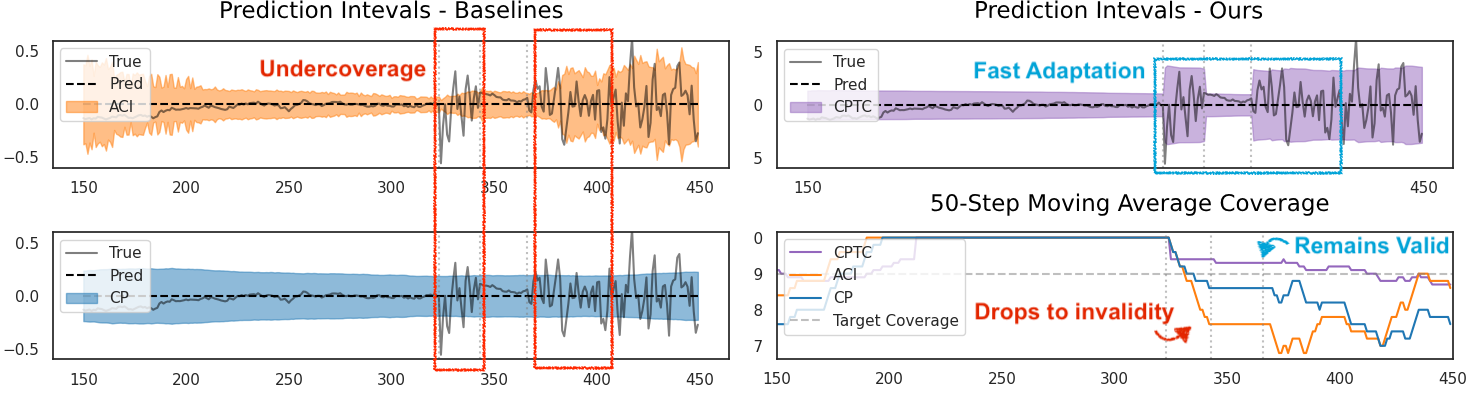
\includegraphics[width=1.01\linewidth]{changepoints/figs/ex/ex_zoom.png}
    \caption{Comparison of the prediction intervals obtained by our algorithm CPTC (purple) against online conformal prediction baselines on synthetic data. The vertical dashed line marks the distribution shifts; ideal behavior is consistent coverage at the horizontal dashed line in the final panel. Bottom right panel shows that CPTC achieves fast adaptation and remains valid when change points occur.}
    \label{fig:cov}
    \vspace{-1em}

\end{figure}
%    \vspace{-2.0em}
%\end{wrapfigure}

%
\vspace{-0.5em}
\begin{itemize}
    \item We propose a new algorithm \textbf{C}onformal \textbf{P}rediction for \textbf{T}ime series with \textbf{C}hange points (CPTC) that utilizes state transition predictions to improve uncertainty quantification for time-series forecasts. Leveraging properties of a SDS model, CPTC consolidates multiple future forecasts to adaptively adjust its prediction intervals when underlying dynamics shift.
    \item We prove that CPTC achieves asymptotic valid coverage, \textit{without assumptions} on the data generation process or state transition model accuracy. When predicted state transitions align well with distribution shifts, CPTC can anticipate uncertainty and adapt faster.
    \item We show strong empirical results on 3 synthetic and 3 real-world datasets. Compared to online conformal prediction baselines, CPTC achieves more robust coverage with comparable prediction intervals sharpness (example in Figure \ref{fig:cov}), and is computationally light.%Compared to  CP algorithms leveraging temporal structures (SPCI \cite{xu2023sequential} and HopCPT \cite{auer2023hopcpt}), CPTC is computationally lighter and more data-efficient.
\end{itemize}

%Conformal prediction produces a $(1-\alpha)$-prediction interval $\Gamma^{1-\alpha}$ for a random variable $y$, which is \textit{valid} if it contains $y$'s true value with high probability:  
%$
%\Prob[y \in \Gamma^{1-\alpha}] \geq 1-\alpha.
%$
%Note that one can make the prediction interval infinitely large to satisfy validity. But for the prediction interval to be useful, we also want to minimize its area while remaining valid; this is known as the \textit{sharpness} of the region. 


% \begin{figure}[h]
%     \centering
%     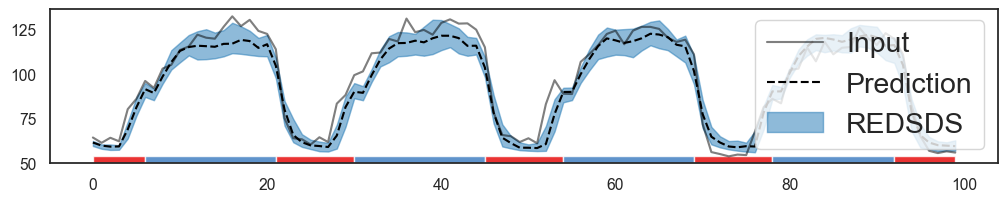
\includegraphics[width=0.9\linewidth]{changepoints/figs/e-prob.png}
%     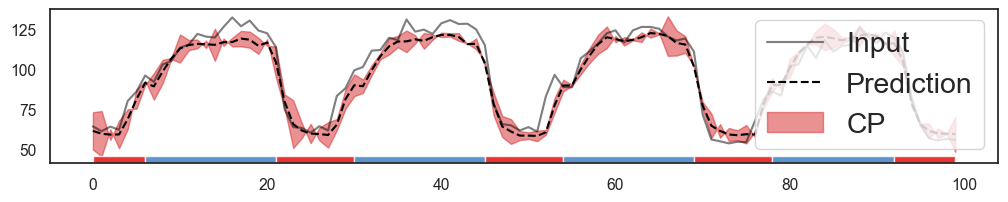
\includegraphics[width=0.9\linewidth]{changepoints/figs/e-cp.png}
%         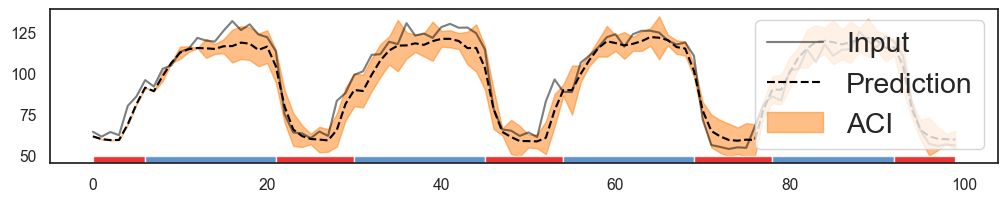
\includegraphics[width=0.9\linewidth]{changepoints/figs/e-aci.png}
%     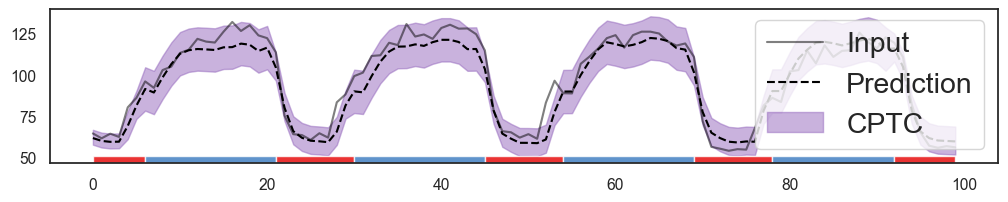
\includegraphics[width=0.9\linewidth]{changepoints/figs/e-ours.png}
%     \caption{Demonstration of uncertainty quantification baselines on hourly electricity demand. Our method (green regions) adapts to different levels of volatility between day and night and whereby achieves more stable coverage over time, whereas ACI (yellow) over-covers during red phases and under-covers during blue.}
%     \label{fig:demonstration}
% \end{figure}


\section{Related Work}
%\vspace{-0.5em}

% \paragraph{Time series forecasting with switching dynamical systems}  State-space models (Fraccaro et al., 2017; Rangapuram
% et al., 2018; de Bézenac et al., 2020; Tang & Matteson, 2021; Klushyn et al., 2021) and recurrent neural
% networks (Salinas et al., 2019; 2020; Rasul et al., 2021b;a) are among the most popular choices to model
% temporal dependencies in time series. 

% However, for these models to generalize and adapt to new changes in the future, it is
% critical to have appropriate inductive biases built into the model. A common approach is to allow state-space models to switch between a discrete set of dynamics, which can be learned from training data.

\vspace{-0.5em}
\paragraph{Probabilistic Forecasting for Time-Series with Change Points.} %Deep learning has enabled substantial advances in time series forecasting. in order to represent the inherent stochasticity of real-world time series data. 
%Probabilistic forecasting methods model distributions over possible outcomes \citep{benidis2022deep}, and have been used widely to build predicting intervals.
%Bayesian Neural Networks (BNN) for uncertainty quantification (UQ) of spatiotemporal forecasts. In practice, Bayesian UQ can be computationally expensive and difficult to optimize, especially for larger networks \citep{lakshminarayanan2017simple, zadrozny2001obtaining}. Therefore, UQ for deep neural network time series forecasts often adopts approximate Bayesian inference such as MC-dropout \citep{gal2016theoretically, gal2017concrete}. Neural process models use neural network to parameterize a stochastic process \citep{garnelo2018conditional,garnelo2018neural, sun2024data}. 
%Method such as (approximate) Bayesian Neural Networks  \citep{wang2019deep, wu2021quantifying, gal2017concrete} and neural process models \citep{garnelo2018conditional, sun2024data} use neural networks to parametrize traditional probabilistic frameworks for time-series forecasting. Other deep-learning models such as DeepAR \citep{salinas2020deepar}, PatchTST \citep{nie2023patchtst}, and Temporal Fusion Transformer \citep{lim2021temporal} directly generate probabilistic forecasts by training the model with pinball loss. 

Probabilistic forecasting has become central to modern time-series analysis by modeling a distribution over future outcomes rather than a single-point forecast \citep{benidis2022deep}. Classic approaches often adopt Bayesian or approximate Bayesian strategies for uncertainty quantification: for instance, Bayesian Neural Networks (BNNs) \citep{wang2019deep, wu2021quantifying, gal2017concrete} or neural process models \citep{garnelo2018conditional, sun2024data} use neural networks to parameterize the underlying stochastic process. Other methods, such as DeepAR \citep{salinas2020deepar}, PatchTST \citep{nie2023patchtst}, or Temporal Fusion Transformer \citep{lim2021temporal}, generate probabilistic forecasts directly by minimizing a pinball loss (i.e., quantile loss), thereby learning predictive distributions.

%\textit{Change points} refer to abrupt distribution shifts in observational time series data \citep{montanez2015inertial}. Detecting and segmenting change points has been studied extensively (see \cite{aminikhanghahi2017survey} for a recent survey), %\citep{adams2007bayesian, agudelo2020bayesian, chiappa2010movement}, 
%whereas modeling time series with change points is typically approached with SSM, and in particular SDS. Recent works in SDS 
%mostly deploy variational inference \citep{johnson2016composing, ansari2021deep, liu2023graph}, using neural networks to parametrize the transition or emission distributions. \cite{sun2024online} studies UQ for change points but in the anomaly detection setting. % to improve flexibility and accelerate inference.

A key challenge arises when \textit{change points} occur - i.e., abrupt distribution shifts in the time series \citep{montanez2015inertial}. Change point detection and segmentation have been studied extensively (beyond our scope, see \citep{aminikhanghahi2017survey} for a recent survey). Modeling time series with change points typically features state-space models (SSM), and in particular switching dynamical systems (SDS) \citep{johnson2016composing, ansari2021deep, liu2023graph}. These SDS approaches use variational inference to fit neural parameterizations of transitions and emission distributions. However, existing probabilistic forecasters often lack strict calibration guarantees and can be overconfident in practice \citep{lakshminarayanan2017simple}, and many require specialized architecture tuning for different tasks, limiting their applicability to real-world UQ challenges.


% Compared to ours and other CP approaches, the drawbacks of the aforementioned methods are: (1) they are not model-free, i.e. special designs of the predictive model and hyper-parameter tuning are required, and (2) they have no theoretical guarantee on calibration and often are overconfident in practice \citep{lakshminarayanan2017simple}.

%SDS models, most often represented as a graphical model, have seen a surge in using neural networks to parameterize transition and emission distributions \citep{johnson2016composing, ansari2021deep, liu2023graph}, to improve flexibility and fast inference. Bayesian and variational inference methods are used extensively in online change point detection \citep{adams2007bayesian, agudelo2020bayesian} and segmentation \citep{chiappa2010movement} as well. 

% Our work focuses on only discrete states, which come with the benefit of interpretability and scalability. Discrete SSMs have been used to address safety-critical distribution shifts, such as reasoning about occlusion in traffic scenes \cite{wei2024navigation}. 

%The challenge of these Bayesian, RNN-, or Transformer-based probabilistic models is that the forecasted probabilities are often uncalibrated or overconfident \citep{lakshminarayanan2017simple}, hence unsuitable for many practical tasks that require guarantees on the uncertainty estimates associated with the forecasts. 

%Frequentist UQ methods emphasize robustness against variations in the data. These approaches either rely on resampling the data or learning an interval bound to encompass the dataset. For time series forecasting UQ, approaches include ensemble methods such as bootstrap \citep{efron2016, bjrnn} and jackknife methods  \citep{jackknife+after, bjrnn}; interval prediction methods include interval regression through proper scoring rules \citep{kivaranovic2020adaptive, wu2021quantifying}, and quantile regression \citep{takeuchi2006nonparametric}, with many recent advances for time series UQ  \citep{tagasovska2019single, gasthaus2019probabilistic,park2022learning, kan2022multivariate}. Many of the frequentist methods produce asymptotically valid confidence regions and can be categorized as distribution-free UQ techniques as they are (1) agnostic to the underlying model and (2) agnostic to data distribution.

\vspace{-0.5em}
\paragraph{Conformal Prediction for time-series.} 
%Conformal prediction (CP), originally introduced in \cite{vovk2005algorithmic}, has become a popular UQ method because of its simplicity, generality,  coverage guarantee, and low computational cost; we refer readers to \cite{angelopoulos2021gentle} for a comprehensive introduction to CP. For time series prediction, \cite{Schaar2021conformaltime, sun2023copula, zhou2024heterogeneous} aims for joint coverage and formulates fixed-length time series problems as exchangeable multi-target forecasts. Enbpi \citep{xu2021conformal} and SPCI \citep{xu2023sequential} assume no change in system dynamics, but in the generating process of the noise or residual that causes uncertainty.  \cite{tibshirani2019conformal} adapts to \textit{known} covariance shift by weighting data using propensity scores. Although theoretically optimal, the algorithm does not apply to real-world problems where propensity scores are difficult to calculate. Adaptive conformal inference (ACI) \citep{gibbs2021adaptive} and its variants \citep{zaffran2022adaptive, gibbs2024conformal, angelopoulos2024pid} consider the online adversarial setting, where they guarantee target marginal coverage without any assumptions on the data generating process. 

Conformal prediction (CP) \citep{vovk2005algorithmic} has emerged as a leading framework for UQ due to its algorithmic simplicity, broad applicability, and finite-sample coverage guarantees; see \cite{angelopoulos2021gentle} for a comprehensive introduction. For time-series forecasting, some works focus on joint coverage over fixed-length horizons \citep{Schaar2021conformaltime, sun2023copula, zhou2024heterogeneous}; others assume stable underlying dynamics and adapt only to shifts in residual distributions \citep{xu2021conformal} . \cite{tibshirani2019conformal} uses known covariate shifts (by propensity weighting) to achieve theoretical coverage, but can fail in settings where the shift mechanism is unknown, which is typical for time series forecasting. \cite{hajihashemi2024multi} introduces a multi-model ensemble CP framework, optimizing model selection within a pool of experts for combined coverage.  CP has also been extended for change-point detection in time series via conformal martingales \citep{vovk2021retrain, volkhonskiy2017inductive}. 

Recent works on online conformal prediction develop online strategies that guarantee marginal coverage for adversarial or nonstationary data streams. ACI \citep{gibbs2021adaptive}, AgACI \citep{zaffran2022adaptive}, DtACI \citep{gibbs2024conformal}, and Conformal PID control \citep{angelopoulos2024pid}  leverage online optimization and have a "reaction" period when distribution shifts. Multivalid Prediction (MVP) \citep{bastani2022practical} provides group coverage guarantees and learns a calibration threshold online, although it can require longer calibration windows. Closer to our work, SPCI \citep{xu2023sequential} learns an autocorrelative estimation of the residual's quantiles through Quantile Random Forest; whereas HopCPT \citep{auer2023hopcpt} condition their conformal interval on similar parts of the time series using a Modern Hopfield Network. The drawback of these two methods is that the regression models are trained during inference time, which (1) requires a long cold start window to learn meaningful associations and (2) is computationally expensive. 
%
Our contribution is a CP algorithm that is computationally light during inference time, and can leverage state prediction capabilities within the SDS model to anticipate and adapt quickly to distribution changes.


%Closest to our work are (1) SPCI \citep{xu2023sequential} learns a time-adaptive estimation of residual quantiles over time, upon leveraging the temporal dependency among them. However, SPCI's theoretical results rely on the properties of a specific quantile learning algorithm, which does not always apply to the time series of interest.(2) Multivalid Prediction (MVP) \citep{bastani2022practical} which guarantees group conditioned coverage in the online adversarial setting. MVP requires a longer sequence as the calibration threshold is learned online. Our work brings their theoretical results into a more practical setting. Our approach also achieves group conditional coverage, which builds upon results from SPCI and MVP. A similar result can be found in \cite{zhou2024heterogeneous} with the name approximate conditional coverage, although only empirical evidence is shown.

%Most relevant to our work is the recent endeavor in generalizing CP to time-series forecasting. \cite{Schaar2021conformaltime} and \cite{sun2023copula} studies . In the case of distribution shifts, ACI \citep{gibbs2021adaptive} and EnbPI \citep{xu2021conformal} developed CP algorithms that relax the exchangeability assumption while maintaining asymptotic validity via online learning (former) and ensembling (later); \cite{zaffran2022adaptive} further improves online adaptation.  \cite{sousa2022general} combines EnbPI with conformal quantile regression \citep{romano2019conformalized} to model heteroscedastic time series. 








\section{Background}


\subsection{Conformal Prediction}
%\sofi{highlight the difference between conformal and split, differenciation}

We briefly review the algorithm and guarantees for conformal prediction, and refer readers to~\cite{angelopoulos2021gentle} for a thorough introduction. In this paper CP refers to \textit{split conformal prediction} (we consider full conformal prediction out of scope, because its computationally complexity renders it nonviable for deep learning settings). The goal of conformal prediction is to produce a \textit{valid} prediction interval (Def.~\ref{def:validity}) for any underlying prediction model.
%
\begin{definition}[Validity]
Given a new data point $(x,y)$, where $y$ is the prediction target and $x$ is the covariates,  and a desired confidence $1-\alpha \in (0,1)$, the prediction interval $\Gamma^{1-\alpha}(x)$ is a subset of $\mathcal{Y}$ containing probable outputs given $x$. The region $\Gamma^{1-\alpha}$ is valid if
%
\begin{equation}\label{eq:coverage}
P (y \in \Gamma^{1-\alpha}(x)) \geq 1-\alpha
 \end{equation}
\label{def:validity}
\end{definition}
%
\vspace{-2em}
Let $\mathcal{D} = \{ (x^i, y^i)\}_{i=1}^n$ be a dataset whose data points $(x^i, y^i)$ are sampled from a distribution on $ \mathcal{X} \times \mathcal{Y}$.  Conformal prediction splits the dataset into a proper training set $\Dtrain$ and a calibration set $\Dcal$. A prediction model $\hat{f}: \mathcal{X} \rightarrow  \mathcal{Y}$ is trained on $\Dtrain$. We use a \textit{nonconformity score} function $A: \mathcal{X} \times  \mathcal{Y} \rightarrow \R_{\geq 0}$ to quantify how well a data sample from calibration \textit{conforms} to the training dataset. Typically, we choose a metric of disagreement between the prediction and the true label as the non-conformity score, such as the Euclidean distance: 
%
\begin{equation}
 A(x,y) \stackrel{\text{e.g.}}{=} d(y,\hat{f}(x)) \stackrel{\text{e.g.}}{=} 
\|y - \hat{f}(x)\|_2 
\label{def:non-c}
\end{equation}
%
Let $\gS = \{A(x^i, y^i)\}_{(x^i, y^i) \in \Dcal}$ denote the set of nonconformity scores of all samples in the calibration set $\Dcal$. %We define a quantile function for nonconformity scores $\gS$ as:
%
During inference time given a new data  $x^{n+1}$, the conformal prediction interval is constructed as in \Eqref{eq:region}, where $Q$ is the empirical quantile function. 
%
\begin{equation}
    \Gamma^{1-\alpha}(x^{n+1}):=  \{ y : A(x^{n+1}, y) \leq Q^{1-\alpha}(\gS \cup \{\infty\})\}  
    \label{eq:region}
\end{equation}
%
% \begin{equation}
%     Q(1-\alpha, \gS) := \text{inf} \{s^*: (\frac{1}{|\gS|} \sum_{s^i \in \gS} \mathbbm{1}_{s^i \leq s^*}) \geq 1-\alpha \}
%     \label{eq:quantile}
% \end{equation}
We say a sample is \textit{covered} if the true value lies in the prediction interval $y^{n+1} \in \Gamma^{1-\alpha}(x^{n+1})$ %and define \textit{coverage} as $P(y^{n+1} \in \Gamma(x^{n+1}))$. 
Conformal prediction is guaranteed to produce valid prediction intervals \citep{vovk2005algorithmic} if the calibration data and test data are exchangeable (in a dataset $\{(x^i, y^i)\}_{i=1}^n$ of size  $n$, any of its $n$! permutations are equally probable).


Conformal prediction has been extended to the online setting. More precisely, the algorithm observes $(x_1, y_1), (x_2, y_2), \ldots$ sequentially, and needs to construct a prediction set $ \Gamma^{1-\alpha}_t$ for $y_t$ at time step $t$. Without making any distributional assumptions on the data generation process, online CP algorithms achieve asymptotic guarantee as \Eqref{eq:aci_convergence}, where $\mathbbm{1}\{\cdot\}$ is the indicator function:
\vspace{-0.5em}
\begin{equation}
\lim_{T \to \infty} \frac{1}{T} \sum_{t=1}^T \mathbbm{1}\{ y_t \notin \Gamma^{1-\alpha}_t(x_t) \} = \alpha  \label{eq:aci_convergence}
\end{equation}

\vspace{-1em}
We refer readers to \cite{angelopoulos2024theoretical} for a summary of theoretical results in this setting.


\subsection{Switching Dynamical Systems for Modeling Time-series with Change Points}
\label{background:sds}
%Switching dynamics systems (SDS), or mixed dynamics systems, is a setting motivated by many real-world scenarios where a single time series model is insufficient to capture the complex and heterogeneous patterns in temporal data. 


\begin{figure}
    \centering
	%\subfloat{\scalebox{0.85}{\input{changepoints/figs/generative.tikz}}}
     \vspace{-2em}
    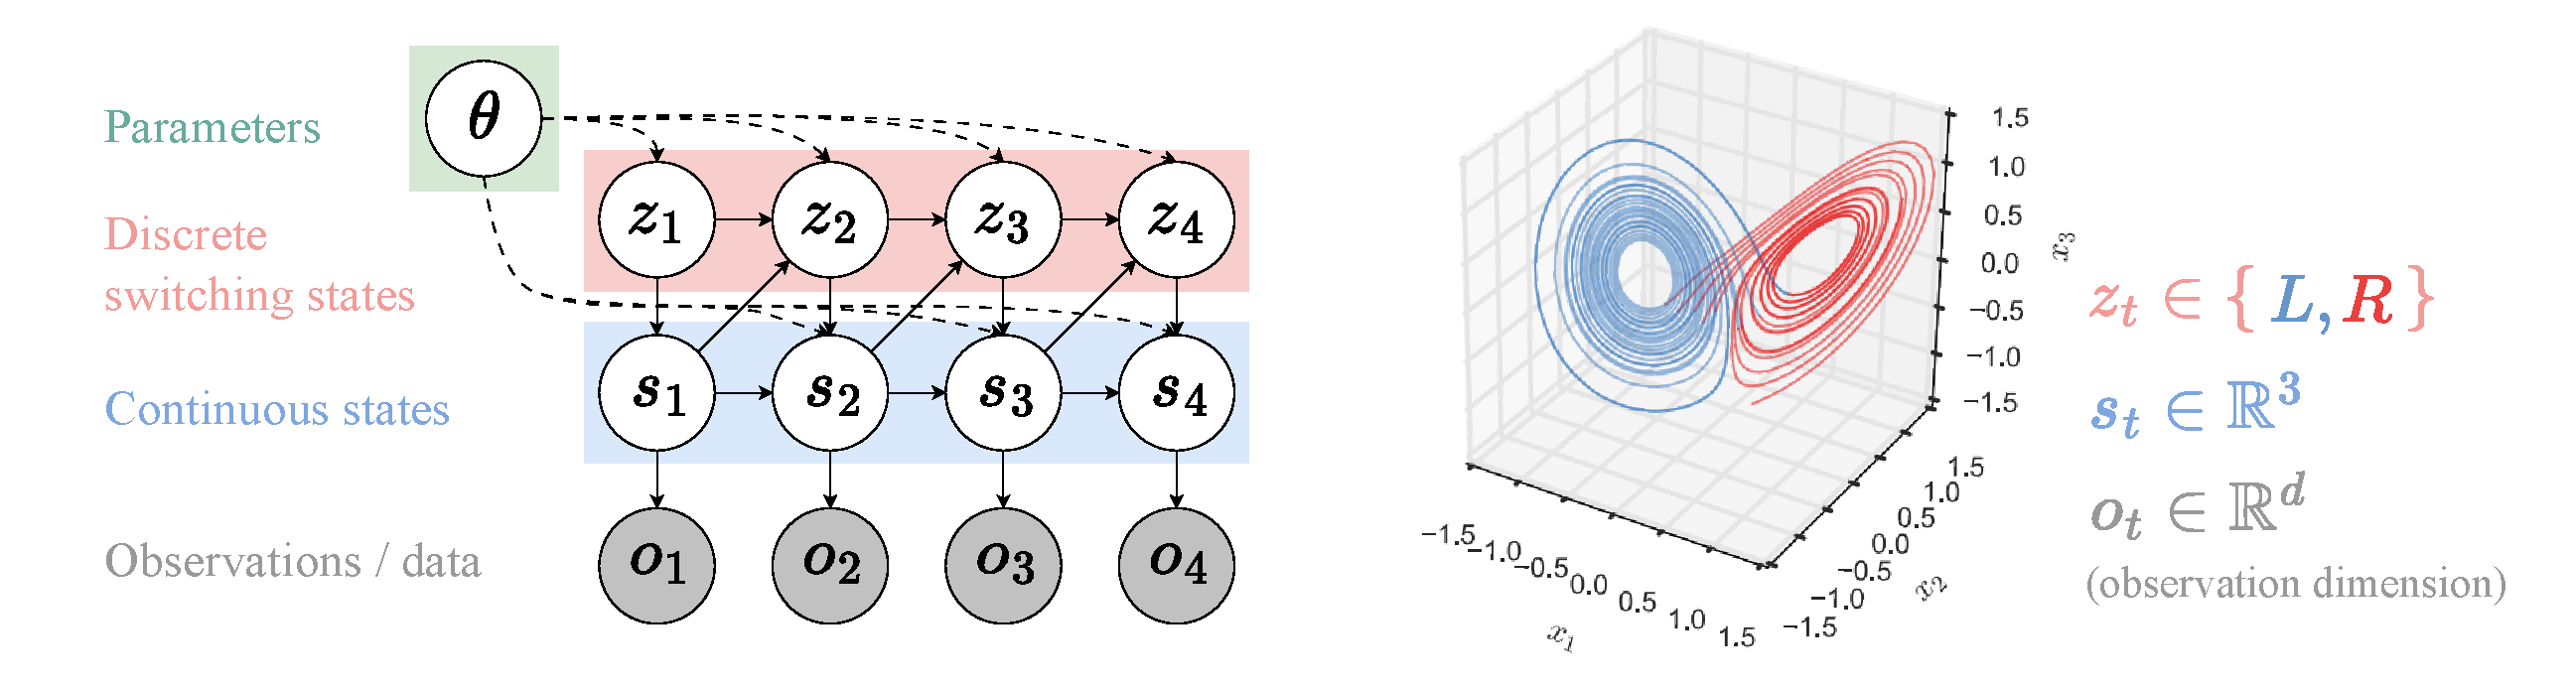
\includegraphics[width=\linewidth]{changepoints/figs/sds.pdf}   \vspace{-1em}
	\caption{(Left) Generative model of the SDS dynamics as in \Eqref{eq:sds}. Shaded circles represent observed  variables; hollow circles are latent variables. (Right) Example to illustrate notation. We show a Lorenz attractor, a canonical nonlinear dynamical system, approximated by a linear SDS \cite{linderman2023slds}.}
	\label{fig:sds_figure}
         \vspace{-1.5em}
\end{figure}

Switching dynamics systems (SDS), or mixed dynamics systems, provide a powerful framework for modeling time series with change points, where the underlying dynamics shift between distinct regimes. SDS assumes the system consists of a total of $K$ different base dynamics. It explicitly incorporates discrete switching \textit{states} to represent the abrupt shifts among base dynamics. We denote the discrete switching states at timestep $t$ as $z_t \in \mathcal{Z}$, $ \mathcal{Z} = \{1, \dots, K\} \subset \mathbb{Z}^+$, to index one of $K$ base dynamical systems, and represent the observed sequence as ${o_1, \ldots, o_T }$ or $o_{1:T}$ for conciseness. %Since continuous states $s_t$ are rarely discussed, we use \textit{state} to refer to discrete states $z_t$ if not otherwise indicated.

There have been many different variations and implementations of SDS.  Classic SDS have \textit{memory-less} state transitions, i.e. $p(z_t|z_{t-1})$ is parameterized by a stochastic transition matrix $\mathbf{A}\in \R ^{K \times K}$. 
This results in an “open loop” system and the state  duration follows a geometric distribution. Recent works have sought to fix this issue, for example by closing the loop using recurrent dependencies on $s_t$ \citep{linderman2016recurrent}, or modeling explicit durations \citep{ansari2021deep}. Our generative model is illustrated in figure \ref{fig:sds_figure}): for generality, we factor out any non-Markovian covariates to model parameters $\theta$. The joint distribution can be factorized as
\vspace{-1em}
\begin{equation} \label{eq:sds}    
\begin{split} 
& P(o_{1:T}, s_{1:T}, z_{1:T} ) =  \prod^T_{t=1} P(o_t | s_t) P(s_t| s_{t-1}, z_t, \theta) P(z_t| s_{t-1}, z_{t-1},\theta)
\end{split}
\end{equation}

\vspace{-1.5em}
where $p(s_1|z_1)p(z_1)$ is the initial state prior. The $K$ dynamical systems have continuous state transition $p(z_t|z_{t-1}, s_{t-1}, \theta)$, and the emission  $p(o_t| s_t)$ can be linear or nonlinear (e.g. parameterized by a neural network). Moreover, the SDS framework naturally supports forecasting both the next observation \(o_{t+1}\) via
$P(o_{t+1}\mid s_{t+1})$
and the next switching state \(z_{t+1}\) via
$P(z_{t+1}\mid s_t, z_t, \theta).$


\section{Conformal Prediction for Time series with Change points (CPTC)}
We introduce CPTC, a novel conformal prediction algorithm that utilizes the state prediction from SDS to improve uncertainty quantification for time series forecasting.
\vspace{-0.5em}
\paragraph{Problem Setting}
% Consider a sequential prediction problem over data generated by the SDS dynamics as illustrated in section \ref{background:sds}, whose observations $o_t \in \R^d$ for all $t$. 
We are given a sequence of observations $o_t \in \R^d$ for all $t$ potentially with  change points.
To be consistent with the standard notation in conformal prediction literature, let 
$\mathcal{X} \subseteq \R^{m}$ denote the input feature domain and $\mathcal{Y} \subseteq \R^d$ the target observation space. $ \mathcal{Z} = \{1, \dots, K\} \subset \mathbb{Z}^+$ indexes one of $K$ underlying states. The input features can include past observations and other environmental covariates.  In our implementations, $m = k \cdot d$ with $k$ being the look back window.

We consider the online conformal prediction setting where we have a sequence of data points from $\mathcal{X} \times \mathcal{Y}$: $(x_1, y_1), $ $(x_2, y_2), \ldots, (x_T , y_T )$. We have a trained state predictor for $\hat{p}(z_t|x_{0:t})$ , a state-conditioned forecaster $\hat{f}:\gX \times \gZ \to \gY$ (a probabilistic SDS model can serve both purposes), and are given a desired confidence level $1-\alpha$. At each time step $t$, we have seen $(x_1, y_1),(x_2, y_2), \ldots,(x_{t-1} , y_{t-1} )$ and the next input feature vector $x_t$. We want to produce an adaptive, time-dependent prediction interval based on input $\Gamma_t(x_t) \subseteq \mathcal{Y}$ for the unseen true target $y_t$, which we will learn at the next time step. Let $z_t \in \gZ$ be the true (latent switching) state at time $t$. %We assume that we have access to a model for probabilistic forecast $\hat{p}(z_t=z|x_{0:t})$ of the latent state at each timestep. %nonconformity score function $A(x, y): \mathcal{X} \times \mathcal{Y} \rightarrow \R_{\geq 0}$   kkfldldldfk;sdf%, denoted as $\hat{z_t}$, and a dynamics forecaster model for each mode $ \hat{f}_z$. 
Our goal is to produce prediction intervals with correct empirical coverage, i.e.    
\vspace{-0.2em}
\begin{equation}
    P (y_t \in \Gamma_t(x_t)) \geq 1-\alpha \; \text{ for any } t\geq 0
    \label{eq:goal}
\end{equation}
\vspace{-2em}
\subsection{Algorithm}
Existing online conformal prediction algorithms often rely on assumptions about how distribution would shift in time series. This is infeasible for data with change points due to  unknown shift mechanism. The main contribution our algorithm makes towards addressing this issue is \textit{anticipating} this type of abrupt shifts. 
Our CPTC algorithm is outlined in pseudo-code in algorithm \ref{alg:cptc}. In this section, we discuss the general procedure and key components of the algorithm. 


%\begin{wrapfigure}{r}{0.5\textwidth}
% \begin{wrapfigure}{L}{0.6\textwidth}
% \begin{minipage}{0.6\textwidth}

\begin{algorithm}[H]%[tb]
   \caption{Conformal Prediction for Time series with Change points (CPTC)}
   \label{alg:cptc}
   \SetAlgoLined
   \KwIn{nonconformity score function $A$, probabilistic state model $\hat{p}(z_t|x_{0:t})$ with prior $\hat{p}(z_0)$, forecaster model $\hat{f}: \mathcal{X}\times \mathcal{Z} \rightarrow \mathcal{Y} $, confidence level $1- \alpha$, learning rate $\gamma$}
   \KwOut{Prediction intervals $\Gamma(x_t)$ for $t \geq 1$}
   
   \For{$z \in \mathcal{Z}$}{
       Initialize $\gS_z \leftarrow \{\}$,  $\alpha_{z,0} \leftarrow \alpha$ 
   }
   \If{exists warm start data $\{(x_t, y_t)\}_{t=-w}^{0}$}{
       \For{$t \in [-w,0]$}{
        $\gS_{z_t} \leftarrow \gS_{z_t} \cup \{A(x_t, y_t)\}$, where $z_t \sim \hat{p}(z_t = z |x_{0:t})$; \tcp{warm start scores} 
       }
   }
   \For{$t \in [1,T]$}{
       \For{$z \in \mathcal{Z}$}{
           $\Gamma_{z,t}(x_t) \leftarrow \{ y : A(x_t, y) \leq Q^{1-\alpha_{z,t}}(\gS_z \cup \{\infty\})\}   $; \tcp{state-specific CP} %Conformal prediction interval with forecaster $\hat{f}(x_t,z)$, confidence level $1-\alpha_{z,t}$, calibrated on $\gS_z$\;
       }
       $\Gamma_t(x_t) \leftarrow$ Aggregate the $\Gamma_{z,t}(x_t)$s by \Eqref{eq:aggregation-average} or \Eqref{eq:aggregation-union}\;
       \KwOut{$\Gamma_t(x_t)$}
       Sample state $\hat{z}_t \sim \hat{p}(z_t|x_{0:t})$; \tcp{state-specific coverage target tracking}
       Update $\alpha_{\hat{z}_t, t+1} \leftarrow \alpha_{\hat{z}_t, t} + \gamma \cdot (\alpha - err_t)$, where $err_t = \mathbbm{1}\{y_t \notin \Gamma_t(x_t)\}$\;
       Update scores $\gS_{\hat{z}_t} \leftarrow \gS_{\hat{z}_t} \cup \{A(x_t, y_t)\}$\;
   }     
   \end{algorithm}
  %   \end{minipage}
  % \end{wrapfigure}



\vspace{-0.5em}
\paragraph{Switching Behavior and SDS Integration.}
We explicitly model the abrupt shift in dynamics with the switching dynamical systems (SDS) to anticipate the change. In our formulation, the latent state \(z_t\) indicates which dynamical regime (out of \(K\) possible regimes) is currently active at time \(t\). Given the SDS formulation (e.g. \Eqref{eq:sds}), we can factor the state transition probability from the conformal prediction process and do calibration for each of the $K$ dynamics separately. The goal in \Eqref{eq:goal} can therefore be written as:
%
\begin{equation}
    \sum_{z\in\gZ} P(y_t \in \Gamma_t(x_t)| z_t=z) \; P(z_t = z|x_{0:t}) \geq 1-\alpha 
\label{eq:factored_goal}
\end{equation}
\vspace{-1.2em}
\paragraph{State Prediction.} The SDS model provides us with the state predictor \(\hat{p}(z_t \mid x_t)\). In practice, SDS models \cite{ansari2021deep, linderman2016recurrent} have existing $z_t$ forecasts that we can extract. For other model architectures, one can modify them to output an extra covariate prediction for the state, or add an auxiliary model to classify or cluster the input space into different regimes. In practice, $z_t$ doesn’t necessarily have to come from a model, and can be any discrete contextual variable such as weekday/weekend/holiday or day/night.

\vspace{-0.5em}
\paragraph{Initialization and Warm Start,} For each switching state $z \in Z$, we initialize (1) a mode-specific set of nonconformity scores $\gS_z$ and (2) the mode-specific confidence level $\alpha_{z,0} = \alpha$. If there are $w$ steps of warm-start data $\{(x_t,y_t)\}_{t=-w}^0$, we initialize the sore sets $\gS_z$ by sampling $z_t \sim \hat{p}(z_t = z |x_{0:t})$ for $t= -w, \ldots, 0$, and inserting $A(x_t,y_t)$ into $\gS_{z_t}$. Depending on the size of the warm-start window and desired properties, practitioners can adjust the warm-starting approach. For example, using the entire warm-start window $\gS_{z} = \{A(x_t,y_t)\}_{t=-w}^0$  for all $z \in \gZ$  will result in better stability but less adaptability to modes. The approach does not change the algorithm's coverage guarantees. 

\vspace{-0.5em}
\paragraph{State-Specific Prediction Intervals.}  At every time step $t\in [1, T]$, CPTC creates state-specific conformal prediction intervals
for all states with nonzero probability. This allows us to generate predictions tailored to the current anticipated dynamics. Specifically, for every state $z\in \gZ$ where $\hat{p}(z|x_{0:t}) > 0$, we first obtain the point prediction through forecaster model $\hat{f}(x_t, z)$, and then the state-specific prediction interval $\Gamma_{z,t}(x_t)$ by calibrating on nonconformity scores set $\gS_z$ to the adaptive confidence level of $1-\alpha_{z,t}$.


\vspace{-0.5em}
\paragraph{Online Conformal Prediction.}
The exchangeability assumption does not apply to the online setting of our work. If we naively calibrate with online data, when the data distribution changes, the coverage probability may deviate from the target level $1-\alpha$. Therefore, we follow online CP methods such as ACI \citep{gibbs2021adaptive} to address this problem by continuously updating $\alpha_{z,t}$ to track a surrogate miscoverage rate $\alpha_{z,t}^*$ as defined in \eqref{eq:alpha_star} (for each state $z$ in our setting), an internal estimate of the target coverage.
%
\begin{equation}
    \alpha^*_{z,t} = \sup\{\beta \in [0, 1] : M_{z,t}(\beta) \leq \alpha\}, \; M_{z,t}(\alpha) = p(A(x_t, y_t) > Q^{1 - \alpha}(\gS_z))  
    \label{eq:alpha_star}
\end{equation}
%
In \eqref{eq:alpha_star} $M_{z,t}$ measures the probability that the true label $y_t$ falls outside the prediction set $\Gamma_{z,t}$ when the predicted state is $z$. %$M_t(\alpha)$ may not be equal to $\alpha$ due to distribution shifts. 
We track $\alpha^*_{z,t}$ over time by updating the estimate $\alpha_{z,t}$ with online optimization. In our implementation, we use the simple update from ACI (\Eqref{eq:aci_update}), though more sophisticated approaches such as \citep{angelopoulos2024pid} may be used in its place without affecting the overall algorithm.
\begin{equation}
\alpha_{\hat{z}_t, t+1} \leftarrow \alpha_{\hat{z}_t, t} + \gamma \cdot (\alpha - err_t), \; \text{where } err_t = \mathbbm{1} \{y_t \notin \Gamma_t(x_t) \}
\label{eq:aci_update}
\end{equation}
Here $\gamma > 0$ is the step size hyperparameter, and $\hat{z}_t \in \gZ, \; \hat{z}_t \sim \hat{p}(z_t = z |x_{0:t})$ is the state at time $t$ sampled to be updated. The update rule increases $\alpha_{\hat{z}_t, t}$ if coverage is too conservative and decreases it otherwise, ensuring that for each $z \in \gZ$, $\alpha_{z,t}$ converges to a value that maintains long-term coverage. 


\vspace{-0.5em}
\paragraph{Aggregation.} We aggregate the prediction intervals for each state $\Gamma_{z,t}(x_t)$ into one final set $\Gamma_{t}(x_t)$ using the weighted level set, as illustrated in \Eqref{eq:aggregation-average}. %The weighted approach results in sharp prediction intervals, but may risk slightly lower coverage if the classifier for $z$ is imperfect.
%
\begin{equation}
\Gamma_t(x_t) :=  \bigl\{ y:  \sum_{z \in \mathcal{Z}}
\hat{p}\bigl(z_t = z \mid x_t\bigr)
\mathbbm{1}\{\,y \in \Gamma_{z,t}(x_t)\} 
\geq 1 - \alpha \bigr\}
\label{eq:aggregation-average}
\end{equation}

\vspace{-0.8em}
Solution to the constraint in \Eqref{eq:aggregation-average}  is the minimal set that achieves the marginal coverage. It can be obtained through discretizing $\mathcal{Y}$ into a fine grid and calculating probability mass at each point, which becomes computationally expensive as the grid resolution or dimensionality increases. For faster computation and in implementation, we approximate the weighted level‐set in \Eqref{eq:aggregation-average} by taking the union of intervals of the most probable states as in \Eqref{eq:aggregation-union}. The two aggregation strategies achieve similar results on all our datasets (Appendix \ref{app:more_experiments}).
%
%Alternatively, we can opt for a more conservative aggregation by taking the union of intervals of the probable states as in  \sofi{explain why they are not far, explain approx eq}
%Alternatively, if finding the set in Eq. \ref{eq:aggregation-average} is challenging or there are high uncertainty for the state classifier, we can opt for a more conservative relaxation. Aggregation by taking the union (Eq. \ref{eq:aggregation-union}) results in larger sets and guaranteed validity over time. 
 \begin{equation}
    \Gamma_t(x_t) \approx \cup_{z\in \mathcal{Z}'_t} \Gamma_{z,t}(x_t), \; 
    \text{where } \mathcal{Z}'_t
=\;\underset{S\subseteq\mathcal Z}{\arg\min}\;\bigl\lvert S\bigr\rvert
\;\text{s.t.}\;\sum_{z\in S}p(z_t=z\mid x_t)\;\ge\;1-\alpha.
    \label{eq:aggregation-union}
\end{equation}
%
\vspace{-1.5em}
\paragraph{Modularity and the role of the state model.} Our algorithm can be viewed as running multiple instances of online conformal inference (lines 14-16 of algorithm \ref{alg:cptc}), one for each underlying state, and adaptively aggregating the confidence intervals when the underlying mode is switching. This differs from the setting where the temporal correlation between residuals needs to be learned online \citep{gibbs2024conformal, bastani2022practical, xu2023sequential, auer2023hopcpt}; the state model allows us to leverage training data for such information. Our algorithm is modular - the state model, forecaster model, and the online adaptive conformal prediction algorithms all operate independently of each other. For example, the state-specific online coverage tracking (line 15 of algorithm \ref{alg:cptc}) can be replaced with other online conformal prediction variants for data-specific applications. Our theoretical guarantees are agnostic to the forecaster models used. %If the forecasters and the state model are re-trained, our algorithm will adapt to the new model while still achieving asymptotic coverage. Section \ref{sec:theory} will elaborate on this claim. 



\subsection{Theoretical analysis}
\label{sec:theory}

In this section, we discuss theoretical guarantees of the CPTC algorithm. In particular, we establish finite-sample validity under exchangeability, asymptotic coverage in dynamic (potentially nonstationary) settings, robustness to imperfect state classification, and faster adaptation to distribution shifts that align with model-predicted state changes. See Appendix \ref{app:proofs} for proofs and theoretical details.

\vspace{-0.5em}
\paragraph{Finite-sample validity under exchangeability.}
We start by showing that when data is exchangeable (e.g. independent and identically distributed), CPTC achieves finite sample validity. The proof is standard based on showing the marginal coverage of split conformal prediction. 

\begin{proposition}[Finite-sample validity under exchangeability] If the data $(x_t, y_t)$, $t \geq 1$ are exchangeable, prediction intervals obtained via Algorithm \ref{alg:cptc} satisfy
\( P(y_t \in \Gamma_t(x_t)) \geq 1-\alpha\).
\label{prop:exchangable}
\end{proposition}

\vspace{-0.5em}
\paragraph{Asymptotic validity without assumptions.}
%\vspace{-0.3em}
Theorem \ref{thm:asymptotic_validity} ensures that CPTC provides reliable uncertainty quantification in the long run \textit{without assumptions on time-series stationarity or accurate state predictions}. (We do assume that the distribution of states and state predictions exhibit stable long-term behavior in Assumption \ref{assump:stationary_distribution}.) We achieve our desiderata of \Eqref{eq:goal} on average as $T$ grows asymptotically, consistent with the results of other online conformal prediction works. 

%
\begin{theorem}[Asymptotic validity of CPTC] \label{thm:asymptotic_validity}
For any sample size \( T \geq 1 \), the CPTC algorithm (with weighted average aggregation) achieves:
\begin{equation*}
    \left| \frac{1}{T} \sum_{t=1}^T \mathbb{E}[err_t] - \alpha \right| \leq  \frac{1}{T} \sum_{z=1}^K  \frac{ 1 - (1-c\gamma)^{|\mathcal{T}_z|}  }{\gamma} |\alpha - \alpha^{*}_z|
    \label{eq:thm1}
\end{equation*}
Where:
\vspace{-4mm}
\begin{itemize}  \setlength{\itemsep}{0pt plus 1pt}
    \item \(\text{err}_t = \mathbbm{1}[Y_t \notin \Gamma_{t}(x_t)]\), the miscoverage rate. 
    \item \( \mathcal{T}_z = \{ t \in \{1, \dots, T\} : \hat{z}_t = z \} \), the set of time steps the predicted state is \( z \).
    \item $\alpha^*_z$ is the optimal miscoverage target for timesteps $\mathcal{T}_z$.
    \item  $c$ is a miscoverage constant in Lemma \ref{lemma:aci_within_states} \cite{gibbs2021adaptive}. 
\end{itemize}
\vspace{-0.5em}
Note the RHS of \Eqref{eq:thm1} decays at a rate of $\mathcal{O}(T)$ and satisfies
 \(
 \lim_{T \to \infty} \left| \frac{1}{T} \sum_{t=1}^T \mathbb{E}[err_t] - \alpha \right|= 0
 \).
\end{theorem}

%Importantly, the algorithm adapts dynamically to stabilize its coverage as the time horizon increases.

\vspace{-0.5em}
\paragraph{Robustness to imperfect state prediction.}
In real-world applications, the state predictor  $\hat{p}(z_t|x_{0:t})$ that plays a large role in our algorithm is often imperfect. The CPTC algorithm accommodates these scenarios by tracking $\alpha^*_{z}$ for each \textit{predicted} mode $z$ with adaptive online updates. Theorem \ref{thm:imperfect_state_predictions} quantifies the effect of imperfect state prediction by showing that the miscoverage rate is bounded by the product of the misclassification rate and state-specific deviations. 
%
\vspace{0.1em}
\begin{theorem}[Finite-Sample Miscoverage Bound with Imperfect State Predictions]\label{thm:imperfect_state_predictions}
For any sample size \( T \geq 1 \), the CPTC algorithm ensures that:
\vspace{-0.2em}
\[
\left| \frac{1}{T} \sum_{t=1}^{T} \mathbb{E}[err_t]  - \alpha \right| \leq \epsilon \cdot \max_z \delta_{z,T}
\]

\vspace{-1em}
Where \( \epsilon = P(\hat{z}_t \neq z_t) \) is the error rate of the state predictions and \( \delta_{z,T} \) is the miscoverage deviation from \( \alpha \) for any predicted state $z$ defined in Lemma \ref{lemma:aci_within_states}. For all $z$, \( \delta_{z,T} \to 0 \) as \( |T| \to \infty \).
%\vspace{-4mm}
% \begin{itemize}\setlength{\itemsep}{0pt plus 1pt}
    %\item \(\text{err}_t := \mathbb{I}\big(Y_t \notin \Gamma_{CPTC}(x_t)\big)\), the miscoverage rate. 
    %\item \( \mathcal{T}_z = \{ t \in \{1, \dots, T\} : \hat{z}_t = z \} \), the set of times when the predicted state is \( z \).
    %\item \( z_t \) denotes the true latent state at time \( t \), and \( \hat{z}_t \) the predicted state. 
%     \item \( \epsilon = P(\hat{z}_t \neq z_t) \) is the error rate of the state predictions.
%     \item \( \delta_{z,T} \) is the miscoverage deviation from \( \alpha \) for any predicted state $z$ defined in Lemma \ref{lemma:aci_within_states}. For all $z$, \( \delta_{z,T} \to 0 \) as \( |T| \to \infty \).
% \end{itemize}
\end{theorem}

Theorem \ref{thm:imperfect_state_predictions} demonstrates that CPTC can maintain asymptotic valid coverage even when state predictions are imperfect, with the bound tightening as state predictions improve or the number of observations per state increases. In practice, improving the accuracy of the state prediction model directly enhances the coverage performance of CPTC. However, even with imperfect state predictions, the algorithm's adaptive calibration mechanism ensures that the overall coverage remains close to the desired level \(1 - \alpha\) as experiments show in Section \ref{sec:accuracy}.

%\subsubsection{Validity for union aggregation}

%As noted in the methodology section, if we use set union as the aggregation approach, CPTC will produce more conservative prediction intervals aiming for overcoverage. 

%By leveraging the union of prediction sets across all possible states, CPTC ensures that the algorithm maintains valid coverage, even in the presence of uncertainty during state transitions.

% \begin{proposition}[Conservative Coverage Guarantee of CPTC on Transition States]
% Note that \(\Gamma_t(x_t) = \bigcup_{z \in Z} \Gamma_{z,t}(x_t)\) is the prediction set produced by the CPTC algorithm at time \(t\).
% then the overall prediction set \(\Gamma_t(x_t)\) provides conservative coverage, meaning:
% \begin{equation}
% P(y_t \in \Gamma_t(x_t)) \geq 1 - \alpha
% \end{equation}
% for all \(t\).
% \end{proposition}

% This is because (1)  \(P(y_t \in \Gamma_{z,t}(x_t) | z_t = z) \geq 1 - \alpha_{z,t}\) for all \(t\) (i.e., the conditional coverage given state \(z\) is at least \(1 - \alpha_{z,t}\)), and (2)  \(\lim_{T_z \to \infty} (1/T_z) \sum_{t=1}^{T_z} \alpha_{z,t} \leq \alpha\) where \(T_z\) is the number of time steps where state \(z\) is predicted. 
\vspace{-0.3em}
\paragraph{Why CPTC? Faster convergence under distribution shifts.}

The strength of the CPTC algorithm is its fast adaptation in dynamic environments with distributional changes. When a distribution shift aligns with a predicted state transition, the structure of CPTC allows the confidence level $\alpha_{z,t}$ to converge to the new target error rate faster compared to purely online methods.

Consider a data stream with a distribution shift occurring at time $t_{{\text{shift}}}$. Let $\alpha^*_{j}$ denote the optimal target error rate for mode $j$ after the shift, and assume that the predicted state $\hat{z}_t$ correctly reflects the shift: $t_{\text{shift}}$ and $\alpha^*_{z} = \alpha^*_{j}$ for $t > t_{{\text{shift}}}$. For conciseness of notation in Theorem \ref{thm:adaptation}, let $\delta_{j,T}$ and $\delta_{ACI,T}$ denote the miscoverage rate \textit{starting from } $t_{\text{shift}}$ for CPTC and ACI respectively.

\vspace{0.1em}
\begin{theorem}[Miscoverage Ratio under State-Coincident Distribution Shift]
Under a state shift from $i$ to $j$ at time step $t_{\text{shift}}$, coinciding with predicted transition, the CPTC algorithm achieves faster convergence to the new target $\alpha^*_{j}$ compared to non-state-aware algorithm ACI at a ratio of:
\[
\frac{\delta_{j,T}}{\delta_{\text{ACI},T}} \leq \frac{|\alpha_{j, t_{\text{shift}}-1}  - \alpha^{*}_{j}|}{|\alpha_{ t_{\text{shift}}-1} - \alpha^{*}_{j}|}
\]
\label{thm:adaptation}
\end{theorem}
\vspace{-1em}
%
The numerator $|\alpha_{j, t_{\text{shift}}-1}  - \alpha^{*}_{j}| \rightarrow 0$ as $T \rightarrow \infty$, when in-state adaptation has converged; but the denominator $|\alpha_{ t_{\text{shift}}-1} - \alpha^{*}_{j}|$ remains greater than zero regardless of the length of the time series. This result highlights the advantage of segmenting nonconformity scores by state: the state-specific $\alpha_{z,t}$ aligns the target miscoverage updates with distribution shifts, allowing CPTC to quickly adjust its prediction intervals. Such accelerated adaptation allows for shorter miscoverage periods and is critical in real-world applications where rapid responses to changing conditions are necessary.
%Theorem \ref{thm:adaptation} shows that CPTC's bound is smaller by a factor that depends on the ratio of the distances of the original $\alpha$ and $\alpha_{i}^*$ from the new optimum $\alpha_{j}^*$, as well as the ratio of the segment lengths.



\section{Experiments}


% \begin{table*}[bh]
% \vspace{-0.8em}
% \caption{Performance on synthetic and real-world datasets with target confidence $1-\alpha = 0.9$ (for horizon $T=200$ for synthetic datasets, $300$ for electricity and traffic, and $60$ for bee, mean $\pm$ standard deviation of the test samples).  Methods that are \textit{invalid} (coverage below $90\%$) are grayed out. Our method achieves a high level of calibration (coverage is close to $90\%$) consistently. }
% \label{tab:baselines}
% \centering
% \resizebox{\textwidth}{!}{%
% \begin{tabular}{ l | c | c  c c c c c } 
% \toprule
% & & RED-SDS & CP & ACI & SPCI  & HopCPT & Ours \\ 
% \midrule\midrule
% \multirow{2}{*}{\begin{tabular}{l}Bouncing  \\ Ball obs.\end{tabular}} & Cov & \color{gray}{59.14 \plusminus 23.75}& \color{gray}{39.27 \plusminus 6.77}& \color{gray}{76.97 \plusminus 1.27}& \color{gray}{37.90 \plusminus 9.78}& \color{gray}{59.45 \plusminus 12.51} &91.03 \plusminus 1.37\\ 
%  & Width & \color{gray}{2.12 \plusminus 0.05}& \color{gray}{1.71 \plusminus 0.93}& \color{gray}{3.67 \plusminus 0.91}& \color{gray}{1.45 \plusminus 0.85}& \color{gray}{1.98 \plusminus 0.90} & 2.13 \plusminus 2.15\\ 
% \midrule
% \multirow{2}{*}{\begin{tabular}{l}Bouncing  \\ Ball dyn.\end{tabular}} & Cov & \color{gray}{43.46 \plusminus 27.18}& \color{gray}{40.41 \plusminus 6.89}& \color{gray}{76.63 \plusminus 0.95}& \color{gray}{53.62 \plusminus 7.75}& \color{gray}{61.12 \plusminus 4.80} &90.44 \plusminus 1.51\\ 
%  & Width & \color{gray}{1.80 \plusminus 0.03}& \color{gray}{0.89 \plusminus 0.45}& \color{gray}{2.97 \plusminus 1.07}& \color{gray}{2.02 \plusminus 0.23}& \color{gray}{2.95 \plusminus 1.12} & 4.92 \plusminus 2.79\\ 
% \midrule
% \multirow{2}{*}{\begin{tabular}{l}3-Mode \\ System\end{tabular}} & Cov & 92.98 \plusminus 3.01& \color{gray}{63.97 \plusminus 5.03}& \color{gray}{86.25 \plusminus 0.84}& \color{gray}{81.72 \plusminus 2.88}& 89.85 \plusminus 2.90 & 93.35 \plusminus 3.51\\ 
%  & Width & 2.08 \plusminus 0.16& \color{gray}{1.46 \plusminus 0.51}& \color{gray}{2.61 \plusminus 0.53}& \color{gray}{3.94 \plusminus 0.85}& 9.07 \plusminus 1.23 &  13.68 \plusminus 2.49\\ 
% \midrule
% \midrule
% \multirow{2}{*}{\begin{tabular}{l}Traffic\end{tabular}} & Cov & \color{gray}{86.55 \plusminus 11.20}& \color{gray}{69.64 \plusminus 2.62}& \color{gray}{88.19 \plusminus 0.33}& 88.24 \plusminus 2.13& 88.91 \plusminus 3.55 & 94.76 \plusminus 4.93\\ 
%  & Width & \color{gray}{2.81 \plusminus 1.54}& \color{gray}{0.32 \plusminus 0.22}& \color{gray}{56.92 \plusminus 25.26}& 4.62 \plusminus 2.28 & 7.50 \plusminus 10.09 & 8.34 \plusminus 14.44\\ 
% \midrule
% \multirow{2}{*}{\begin{tabular}{l}Electricity\end{tabular}} & Cov & \color{gray}{75.46 \plusminus 14.23}& \color{gray}{68.88 \plusminus 3.12}& \color{gray}{87.94 \plusminus 0.34}& \color{gray}{86.62 \plusminus 2.97} & \color{gray}{86.50 \plusminus 2.66} & 92.62 \plusminus 6.14\\ 
%  & Width & \color{gray}{87.47 \plusminus 119.95}& \color{gray}{58.62 \plusminus 456.89}& \color{gray}{28.28 \plusminus 169.33}& \color{gray}{371.69 \plusminus 305.86}& \color{gray}{155.71 \plusminus 130.43} & 166.88 \plusminus 129.07 \\ 
% \midrule
% \multirow{2}{*}{\begin{tabular}{l}Dancing \\ Bees\end{tabular}} & Cov & 90.79 \plusminus 5.03& \color{gray}{65.58 \plusminus 7.05}& \color{gray}{75.16 \plusminus 3.33}& \color{gray}{79.2 \plusminus 0.3} & \color{gray}{72.11 \plusminus 1.84} & 93.43 \plusminus 11.42 \\
%  & Width & 0.27 \plusminus 0.05& \color{gray}{0.12 \plusminus 0.01}& \color{gray}{1.77 \plusminus 1.38}& \color{gray}{1.77 \plusminus 1.38} & \color{gray}{1.06 \plusminus 0.51} & 1.15 \plusminus 0.56 \\
% \bottomrule
% \end{tabular}
% }
% \vspace{-0.5em}
% \end{table*}

\begin{table*}[bh]
\vspace{-0.8em}
\caption{Performance on synthetic and real-world datasets with target confidence $1-\alpha = 0.9$ (for horizon $T=200$ for synthetic datasets, $300$ for electricity and traffic, and $60$ for bee, mean $\pm$ standard deviation of the test samples).  Methods that are \textit{invalid} (coverage below $90\%$) are grayed out. Our method achieves a high level of calibration (coverage is close to $90\%$) consistently. }
\label{tab:baselines}
\centering
\resizebox{\textwidth}{!}{%
\begin{tabular}{ l | c | c  c c c c c } 
\toprule
& & RED-SDS & CP & ACI & SPCI  & HopCPT & Ours \\ 
\midrule\midrule
\multirow{2}{*}{\begin{tabular}{l}Bouncing  \\ Ball obs.\end{tabular}} & Cov & \color{gray}{16.90 \plusminus 12.96} & \color{gray}{87.67 \plusminus 6.54} & \color{gray}{89.82 \plusminus 2.95} & \color{gray}{87.13 \plusminus 4.79} & \color{gray}{59.45 \plusminus 12.51} & 90.15 \plusminus 1.19\\ 
 & Width & \color{gray}{1.60 \plusminus 0.07} & \color{gray}{10.54 \plusminus 3.19} & \color{gray}{3.85 \plusminus 2.60} & \color{gray}{2.82 \plusminus 0.41} & \color{gray}{1.98 \plusminus 0.90} & 3.71 \plusminus 0.98\\ 
\midrule
\multirow{2}{*}{\begin{tabular}{l}Bouncing  \\ Ball dyn.\end{tabular}} & Cov & \color{gray}{13.20 \plusminus 11.50} & \color{gray}{86.45 \plusminus 12.28} & \color{gray}{89.38 \plusminus 2.56} & \color{gray}{53.62 \plusminus 7.75} & \color{gray}{61.12 \plusminus 4.80} & 90.47 \plusminus 2.30\\ 
 & Width & \color{gray}{1.37 \plusminus 0.05} & \color{gray}{11.49 \plusminus 4.39} & \color{gray}{2.27 \plusminus 1.65} & \color{gray}{2.02 \plusminus 0.23} & \color{gray}{2.95 \plusminus 1.12} & 1.76 \plusminus 0.71\\ 
\midrule
\multirow{2}{*}{\begin{tabular}{l}3-Mode \\ System\end{tabular}} & Cov & 93.02 \plusminus 3.04 & \color{gray}{63.98 \plusminus 5.04} & \color{gray}{89.90 \plusminus 2.25} & \color{gray}{84.90 \plusminus 5.41} & 89.85 \plusminus 2.90 & 94.96 \plusminus 1.96\\ 
 & Width & 2.08 \plusminus 0.16 & \color{gray}{1.46 \plusminus 0.50} & \color{gray}{6.40 \plusminus 1.92} & \color{gray}{3.70 \plusminus 0.89} & 9.07 \plusminus 1.23 & 2.45 \plusminus 0.72\\ 
\midrule
\midrule
\multirow{2}{*}{\begin{tabular}{l}Traffic\end{tabular}} & Cov & \color{gray}{23.15 \plusminus 10.95} & \color{gray}{87.06 \plusminus 3.71} & 90.01 \plusminus 0.87 & \color{gray}{84.38 \plusminus 2.47} & 88.91 \plusminus 3.55 & 92.38 \plusminus 1.24\\ 
 & Width & \color{gray}{0.05 \plusminus 0.02} & \color{gray}{21.91 \plusminus 10.42} & 27.81 \plusminus 54.08 & \color{gray}{5.32 \plusminus 1.95} & 7.50 \plusminus 10.09 & 7.92 \plusminus 2.98\\ 
\midrule
\multirow{2}{*}{\begin{tabular}{l}Electricity\end{tabular}} & Cov & \color{gray}{62.85 \plusminus 13.67} & \color{gray}{85.69 \plusminus 6.17} & \color{gray}{89.79 \plusminus 0.83} & \color{gray}{84.10 \plusminus 2.77} & \color{gray}{86.50 \plusminus 2.66} & 91.22 \plusminus 1.29\\ 
 & Width & \color{gray}{162.67 \plusminus 811.73} & \color{gray}{366.05 \plusminus 2280.45} & \color{gray}{45.74 \plusminus 279.21} & \color{gray}{228.14 \plusminus 1207.58} & \color{gray}{155.71 \plusminus 130.43} & 139.75 \plusminus 620.44\\ 
\midrule
\multirow{2}{*}{\begin{tabular}{l}Dancing \\ Bees\end{tabular}} & Cov & \color{gray}{84.92 \plusminus 6.84} & \color{gray}{79.86 \plusminus 20.73} & \color{gray}{86.25 \plusminus 8.10} & \color{gray}{79.20 \plusminus 0.30} & \color{gray}{72.11 \plusminus 1.84} & 92.64 \plusminus 3.19\\
 & Width & \color{gray}{0.25 \plusminus 0.02} & \color{gray}{1.65 \plusminus 0.58} & \color{gray}{4.79 \plusminus 4.02} & \color{gray}{1.77 \plusminus 1.38} & \color{gray}{1.06 \plusminus 0.51} & 0.79 \plusminus 0.27\\
\bottomrule
\end{tabular}
}
\vspace{-0.5em}
\end{table*}
\vspace{-0.5em}
\paragraph{Baselines.} We selected the following baseline methods. \textbf{RED-SDS} (Recurrent Explicit Duration Switching Dynamical System) \cite{ansari2021deep} is a state-of-the-art Bayesian model that learns state transitions (implementation details in Appendix \ref{app:redsds}). We also use REDSDS as the base predictor for mode switching for our method in the experiments. \textbf{CP} is a generalization of conformal prediction to the online setting, also known as Online Sequential Split Conformal Prediction in \cite{zaffran2022adaptive}. We choose \textbf{ACI} \citep{gibbs2021adaptive} to represent online CP algorithms leveraging online optimization. \textbf{SPCI} \citep{xu2023sequential} and \textbf{HopCPT} \cite{auer2023hopcpt} are state-of-the-art CP algorithms that learns adaptive predictive intervals by quantile regression and Modern Hopfield Networks learned from the time series respectively. 
% \vspace{-0.5em}
% \begin{itemize}
%     \item Recurrent Explicit Duration Switching Dynamical System (RED-SDS) \citep{ansari2021deep}: State-of-the-art Bayesian model that learns state transitions. We also use REDSDS as the base predictor for mode switching for our method in the experiments. 
%     \item CP: A generalization of inductive conformal prediction to the online setting, also known as Online Sequential Split Conformal Prediction in \cite{zaffran2022adaptive}.
%     \item Adaptive conformal inference (ACI) \citep{gibbs2021adaptive}: A primary example of an online conformal prediction algorithm by leveraging online optimization. Similar methods include AgACI \citep{zaffran2022adaptive}, DtACI \citep{gibbs2024conformal}, and Conformal PID control \citep{angelopoulos2024pid}, who  display similar behavior and are thus grouped under this category.
%     \item SPCI \citep{xu2023sequential}: sequential  CP algorithm that handles drift in data distribution by predicting the quantile of a future residual. SPCI is proven to achieve better or comparable results with other state-of-the-art conformal prediction methods for time series \citep{xu2021conformal, lee2024kernel}.
%     \item HopCPT \
% \end{itemize}
%  %
\vspace{-0.5em}
\paragraph{Metrics.}
We evaluate calibration and sharpness for each method. For \textit{calibration}, we report the empirical coverage on the test set. Coverage should be as close to the desired confidence level $1-\alpha$ as possible.
$
 \mathrm{Coverage}= \frac{1}{T} \sum_{t=1}^T \mathbbm{1} (y_t \in \Gamma_t (x_t))
$
   
For \textit{sharpness}, we report the average width or area of the Prediction Intervals (PI). The measure should be as small as possible while being valid (coverage maintains above the specified confidence level). 
$
\mathrm{Width} = \frac{1}{T} \sum_{t=1}^T  | \Gamma_t(x_t)|
$

%To analyze more fine-grained dynamics of the prediction intervals, we also visualize the \textit{rolling coverage and width} over a smaller window size. They reflect the stability of the methods' coverage.

\vspace{-0.5em}
\paragraph{Datasets.} The three synthetic datasets are designed with increasing randomness in mode changes, challenging the adaptivity of CPTC. \textbf{Bouncing Ball} is comprised of univariate time series encoding the height of a ball bouncing between two walls with constant velocity and elastic collisions, following \cite{dong2020collapsed, ansari2021deep}. The two switching states are going up/down, each associated with a different level of Gaussian noise added to observation (Bouncing Ball obs), or the underlying dynamics (Bouncing Ball dyn) which induces uncertainty in the phase as well.  
\textbf{3-mode system} is a switching linear dynamical system with 3 switching states, where each mode samples from a Poisson distribution for duration. 

For real-world datasets, the \textbf{Electricity} and \textbf{Traffic} datasets from \citep{Dua2017UCI} have hourly frequency and exhibit seasonality both in terms of the time series itself and volatility. The \textbf{honey bee trajectory} dataset  \citep{oh2008learning} is the most complex, composed of 4-dimensional trajectories with length averaging to 900 frames, where the bees' dance can be decomposed into ``left turn”, ``right turn” and ``waggle”.

Illustrations of the datasets and detailed description can be found in Appendix \ref{app:exp}. The warm-start window for synthetic and real datasets are 50 and 100 time steps respectively (excluding bees, whose $w=15$). The datasets represent a diverse set of scenarios to demonstrate the robustness and versatility of CPTC, capturing the complexity and variability of practical time-series forecasting problems.%, such as seasonality, nonlinear dynamics, and irregular state durations. 

\vspace{-0.5em}
\subsection{Analysis of Coverage and Sharpness Results}
\vspace{-0.2em}
Results for uncertainty quantification in table \ref{tab:baselines} show that we achieve significantly better validity on all datasets compared to baselines. RED-SDS's intervals fail due to lack of calibration, a common pitfall of probabilistic methods (shown also in \cite{xu2023sequential}). CP's under-coverage shows that the data are not exchangeable. In the pretense of change points, ACI's coverage fluctuates dramatically and did not converging within the horizon (more visualizations in Appendix \ref{app:pictures}).  For SPCI and HopCPT, which also guarantees asymptotic validity, the invalidity is likely because they are designed for large datasets ($T \geq 10,000$ for HopCPT), and did not have enough data to react or learn useful residual patterns for the relatively short prediction horizon of our datasets ($T=200$ for synthetic datasets, 300 for electricity and traffic, and 60 for bees).  Figure \ref{fig:demonstration} provides a qualitative example of how the prediction intervals compare across different methods. Our method (purple shaded regions) does not over-cover during nonvolatile hours, nor under-cover during busy ones, as does ACI. %More visualizations can be found in Appendix \ref{app:pictures}, in which we showcase how CPTC anticipates uncertainty during state changes to mitigate miscoverage.

\begin{figure}[t]
    \vspace{-0.5em}
    \centering
    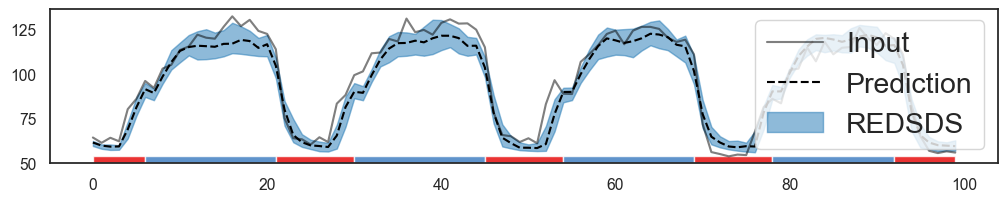
\includegraphics[width=0.49\linewidth]{changepoints/figs/e-prob.png}
    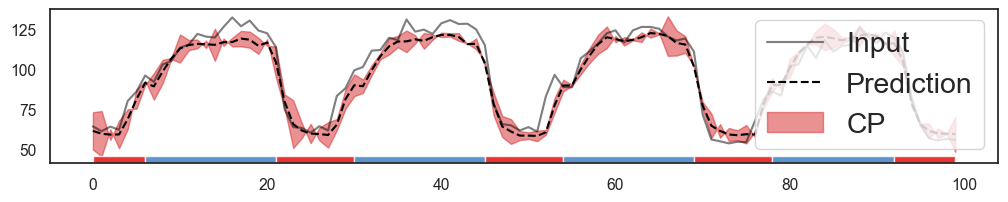
\includegraphics[width=0.49\linewidth]{changepoints/figs/e-cp.png}
    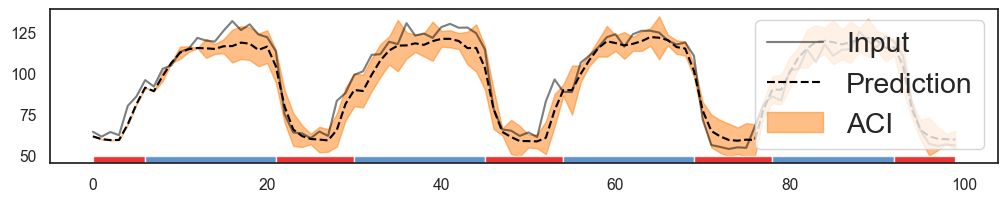
\includegraphics[width=0.49\linewidth]{changepoints/figs/e-aci.png}
    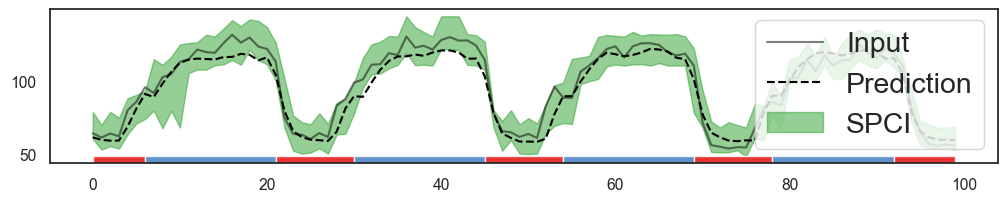
\includegraphics[width=0.49\linewidth]{changepoints/figs/e-spci.png}
    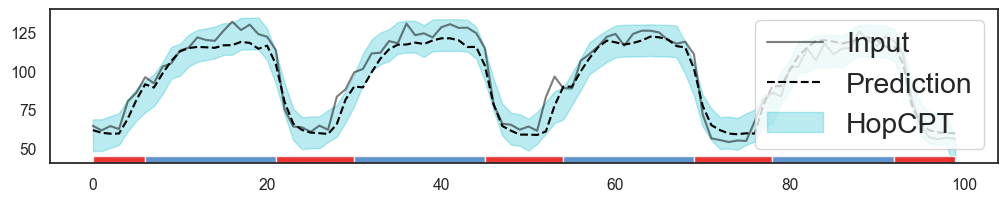
\includegraphics[width=0.49\linewidth]{changepoints/figs/e-hop.png}
    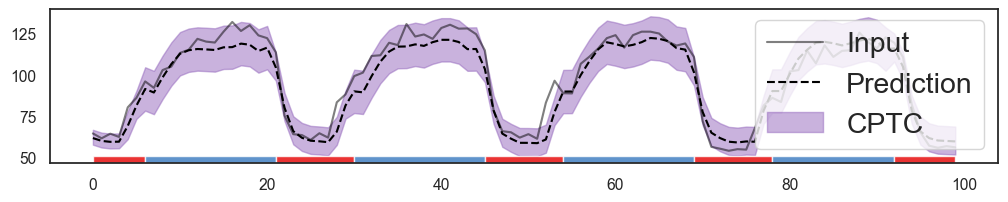
\includegraphics[width=0.49\linewidth]{changepoints/figs/e-ours.png}
    \vspace{-0.5em}
    \caption{\textbf{Visualization of prediction intervals on the Electricity hourly demand dataset.} The red and blue bars in the bottom reflects the underlying switching state of day and night. Our method (purple) adapts to different levels of volatility between day and night, and achieves stabler coverage over time, whereas ACI (yellow) over-covers during the night and under-covers at change points.}
    \label{fig:demonstration}
\vspace{-1em}
\end{figure}


 
%\sofi{Some more visualizations}
%\subsection{Ablation study on aggreagation methods} 
%\sofi{Ablation study on aggreagation methods, ablation on sequence length?}

\vspace{-0.6em}
\subsection{Ablation Studies}
\label{sec:accuracy}
\vspace{-0.5em}
\paragraph{Robustness to $p(\hat{z})$ accuracy.} We conduct ablation studies on the 3 synthetic datasets of which we have ground truth underlying states. As shown in table \ref{tab:z_exp}, it is evident that increasing the error in the state prediction does not affect the coverage performance. This verifies the robustness of our algorithm and theoretical results (Theorem \ref{thm:asymptotic_validity} and \ref{thm:imperfect_state_predictions}). Table \ref{tab:z_exp_area} further shows that the error of state prediction reflects on the width of the prediction intervals: while remaining the same level of coverage, the better the state predictions, the sharper the intervals.

\vspace{-1.5em}
\begin{minipage}{0.58\textwidth}
\begin{table}[H]
    \caption{Coverage of CPTC for using ground truth (GT) labels and with various levels of injected noise, on synthetic data with $T=200$. We can see that coverage performance does not change significantly with error in state prediction. }   
    \vspace{0.4em}
    \label{tab:z_exp}
    \centering
    \resizebox{\textwidth}{!}{%
    \begin{tabular}{c|c c c}
        \toprule
        & Ground truth state labels & GT w/ $20\%$ error & GT w/ $50\%$ error \\ 
        \midrule
        BB obs.  & 90.31 \plusminus 1.27 & 90.27 \plusminus 1.30 & 90.13 \plusminus 1.40 \\ 
        BB dyn.  & 90.34 \plusminus 0.93 & 90.32 \plusminus 0.96 & 90.33 \plusminus 1.05 \\ 
        3-mode  & 92.67 \plusminus 1.52 &  92.70 \plusminus 1.63  & 92.53 \plusminus 1.54 \\ 
        \bottomrule
    \end{tabular}
    }
\end{table}

\end{minipage}
\hfill
\begin{minipage}{0.38\textwidth}
\begin{table}[H]
    \centering
    \caption{Interval width under the same setting. While the coverage guarantee is the same, the more accurate the state prediction is, the sharper the intervals.}
    \vspace{0.4em}
    \label{tab:z_exp_area}
    \resizebox{\textwidth}{!}{%
    \begin{tabular}{c| c c c}
        \toprule
        & GT & w/ $20\%$ err & w/ $50\%$ err\\ 
        \midrule
        BB obs. & 3.61 \plusminus 0.93 & 3.75 \plusminus 0.99 & 3.94 \plusminus 1.17 \\ 
        BB dyn. & 2.09 \plusminus 0.60 & 2.15 \plusminus 0.62 & 2.18 \plusminus 0.65 \\ 
        3-mode & 2.04 \plusminus 0.67 &  2.19 \plusminus 0.76  & 2.27 \plusminus 0.89 \\ 
        \bottomrule
    \end{tabular}
    }       
\end{table}
\end{minipage}

\vspace{0.5em}
Additional ablation studies are presented in Appendix \ref{app:more_experiments}. On \textbf{Aggregation Methods} (by discretization as \Eqref{eq:aggregation-average} or union as \Eqref{eq:aggregation-union}), we found that on our benchmark datasets, union is a close proximation of the true objective, and CPTC achieves similar width and coverage on a sampled subset. For \textbf{Long Horizon Forecasting} where $T \geq 10,000$, our method still achieves valid and stable coverage, but have wider PI width compared to SPCI an HopCPT. They achieve this by frequently re-training their models online, which CPTC does not and is less computationally demanding.

\section{Conclusion and Discussion}

In this paper, we introduced Conformal Prediction for Time-series with Change points (CPTC), a novel conformal prediction algorithm for uncertainty quantification in non-stationary time series. By leveraging state information in switching dynamics systems models, CPTC offers improvements in adaptivity over existing conformal prediction methods. Our theoretical guarantees ensure validity \textit{without assumptions} on time-series stationarity or accurate
state predictions. Empirical results corroborate our theory and demonstrate the effectiveness of CPTC across diverse synthetic and real-world datasets, achieving robust coverage under distributional shifts with comparable sharpness compared to state-of-the-art baselines. The adaptivity advantage is most pronounced in shorter time series, when baselines require more data to react or learn temporal correlations. %CPTC as a versatile tool for time-series UQ in dynamic and complex environments. 
% achieving robust coverage under distributional shifts with comparable sharpness. The adaptivity advantage is  especially on medium-length time series.  while empirical results demonstrate the effectiveness of CPTC across diverse synthetic and real-world datasets. 

Limitations of CPTC include (1) slower convergence rate in scenarios with frequent or unpredictable state transitions, as the algorithm requires sufficient observations within each state to achieve optimal calibration and sharpness, (2) wider prediction interval width when applied to very long time series compared methods specialized for such scenarios (e.g. HopCPT), and (3) requirement of a state prediction model, making our method primarily applicable to SDS models and discrete SSMs. Future work could explore extending the framework to continuous states and the theoretical implications thereof, and studying the decision theoretic properties of using conformal prediction for safety-critical applications requiring real-time adaptation.

%\section*{Acknowledgement}

% \clearpage

% \section*{Acknowledgments and Disclosure of Funding}

% This work was supported in part by the U.S. Army Research Office under Army-ECASE award W911NF-07-R-0003-03, the U.S. Department Of Energy, Office of Science, IARPA HAYSTAC Program, NSF Grants SCALE MoDL-2134209, CCF-2112665 (TILOS), \#2205093, \#2146343, and \#2134274, as well as CDC-RFA-FT-23-0069 from the CDC's Center for Forecasting and Outbreak Analytics. 

% \bibliography{ref.bib}
% \bibliographystyle{abbrv}

% \appendix
\section{Appendix}
\clearpage
\onecolumn

\section{Theoretical Results and Proofs}
\label{app:proofs}

\subsection{Setup and Notation}

Let \( z_t \in \mathcal{Z} = \{1, \dots, K\} \) denote the unobserved discrete mode,  \( x_t \in \mathcal{X} \) denote the continuous state, and \( y_t \in \mathcal{Y} \) the observation at time $t$. We assume we have access to a probabilistic model \( \hat{p}(z_t | X_{1:t-1}) \) that estimates the mode $\hat{z}_t$.

For a target coverage rate \( 1 - \alpha \), let \( \Gamma_{t}(X_t) \) be the prediction set at time \( t \). We define the miscoverage indicator \( M_t \) as follows, and aim to bound the overall miscoverage rate over \( T \) time steps:
\[
M_t = \frac{1}{T} \sum_{t=1}^T err_t, \quad \text{where} \quad err_t := \mathbbm{1}\big(Y_t \notin \Gamma_{t}(X_t)\big),
\]



\subsection{Proofs: Lemma}

In practical scenarios, the state prediction model may not be perfectly accurate. We now analyze the impact of imperfect state predictions on the coverage guarantees of the CPTC algorithm.
 
We derive the following lemma from the convergence result of Proposition 4.1 in \cite{gibbs2021adaptive} with two additional assumptions also according to \cite{gibbs2021adaptive}: (1) the existence of a single fixed optimal target $a^* \in [0,1]$, and (2) $\mathbb{E} [err_t | a_t] = M(a_t)$. These are reasonable assumptions that allow us to quantify distribution shifts and are necessary for analyzing adaptation behavior  (whereas proposition 4.1 itself is a worst-case upper bound.) We refer the readers to the original paper for the complete derivation. 


\begin{lemma}[Adaptive Conformal Inference Miscoverage Bound Within Predicted States]\label{lemma:aci_within_states} Let \( \mathcal{T}_z = \{ t \in \{1, \dots, T\} : \hat{z}_t = z \} \) denote the set of times when the predicted state is \( z \). For any \( T > 1 \) and predicted state \( \hat{z}_t = z \), the Adaptive Conformal Inference (ACI) algorithm ensures that there exists a constant \( \delta_{z, T} \) such that:
 \[ 
\left| \frac{1}{|\mathcal{T}_z|} \sum_{t \in \mathcal{T}_z} \mathbb{E}[err_t] - \alpha \right| \leq \delta_{z, T}
\]

Explicitly, 
\[
\delta_{z,T} =  \frac{1 - (1-c\gamma)^{|\mathcal{T}_z|}}{|\mathcal{T}_z| \gamma} |\alpha - \alpha^{*}_z|
\]
where 
\begin{itemize}
    \item  $\alpha^*_z$ is the optimal miscoverage target for timesteps $\mathcal{T}_z$.
    \item $\gamma$ is the step size
    \item $c$ the miscoverage constant.
\end{itemize}  Note that $\delta_{z,T}$ decays at a rate of $\mathcal{O}(T)$ and satisfies
$ \lim_{\mathcal{T}_z \to \infty} \delta_{z,T} = 0$.

\end{lemma}

\subsection{Proof of Theorem \ref{thm:asymptotic_validity}}

\begin{theorem*}[
\ref{thm:asymptotic_validity} Asymptotic validity of CPTC ]
For any sample size \( T \geq 1 \), without placing any assumptions, the CPTC algorithm ensures that:
\[  
\left| \frac{1}{T} \sum_{t=1}^T \mathbb{E}[err_t] - \alpha \right| \leq \frac{1}{T} \sum_{z=1}^K    |\mathcal{T}_z | \delta_{z,T}  = \frac{1}{T} \sum_{z=1}^K  \frac{ 1 - (1-c\gamma)^{|\mathcal{T}_z|}  }{\gamma} |\alpha - \alpha^{*}_z|
\]
which decays at a rate of $\mathcal{O}(T)$ and satisfies
 \[
 \lim_{T \to \infty} \left| \frac{1}{T} \sum_{t=1}^T \mathbb{E}[err_t] - \alpha \right|= 0.
 \]
\end{theorem*}

To prove theorem \ref{thm:asymptotic_validity}, we assume that both the distribution of the underlying modes $z$ and the predictions $\hat{z}$ is stationary (Assumption \ref{assump:stationary_distribution}). 

\begin{assumption}[Stationary Distribution of States]\label{assump:stationary_distribution}
The sequence of true states \( \{z_t\} \) has a stationary distribution \( \pi(z) \), and the sequence of predicted states \( \{\hat{z}_t\} \) also has a stationary distribution \( \hat{\pi}(z) \). Specifically:
\[
\forall z, \in \mathcal{Z}, \quad \lim_{t \to \infty} p(z_t = z) = \pi(z), \quad \lim_{t \to \infty} p(\hat{z}_t = z) = \hat{\pi}(z),
\]
\end{assumption}


This assumption is well-justified in practical scenarios where the sequence of observations and predictions arises from processes that, while non-stationary over short intervals, exhibit stable long-term behavior. In time-series or dynamic environments, regularities in data generation or prediction models often lead to empirically observed stationarity in distributions. While restrictive, this assumption aligns with prior work in sequential and online prediction frameworks, where stationarity assumptions are standard to derive theoretical guarantees.

 
\begin{proof}[Proof of Theorem \ref{thm:asymptotic_validity}]
Let \( \mathcal{T}_z = \{ t \in \{1, \dots, T\} : \hat{z}_t = z \} \) represent the set of timesteps when the predicted state is \( z \). For the total number of timesteps \( T \), the overall miscoverage error can be expressed as:
\begin{align*}
\frac{1}{T} \sum_{t=1}^T \mathbb{E}[err_t] & = \frac{1}{T} \sum_{z=1}^K \sum_{t \in \mathcal{T}_z} \mathbb{E}[err_t]\\
&= \frac{1}{T} \sum_{z=1}^K |\mathcal{T}_z| \left( \frac{1}{|\mathcal{T}_z|} \sum_{t \in \mathcal{T}_z} \mathbb{E}[err_t] \right).
\end{align*}

From Lemma \ref{lemma:aci_within_states}, for any predicted state \( z \), the miscoverage within \( \mathcal{T}_z \) satisfies:
\[
\left| \frac{1}{|\mathcal{T}_z|} \sum_{t \in \mathcal{T}_z} \mathbb{E}[err_t] - \alpha \right| \leq \delta_{z,T},
\]
where:
\[
\delta_{z,T} = \frac{1 - (1-c\gamma)^{|\mathcal{T}_z|}}{|\mathcal{T}_z| \gamma} |\alpha - \alpha^{*}_z|.
\]

Substituting this bound into the overall miscoverage error, we obtain:
\[
\left| \frac{1}{T} \sum_{t=1}^T \mathbb{E}[err_t] - \alpha \right| \leq \frac{1}{T} \sum_{z=1}^K |\mathcal{T}_z| \delta_{z,T}.
\]

Expanding \( \delta_{z,T} \), the overall bound becomes:
\[
\left| \frac{1}{T} \sum_{t=1}^T \mathbb{E}[err_t] - \alpha \right| \leq \frac{1}{T} \sum_{z=1}^K \frac{ 1 - (1-c\gamma)^{|\mathcal{T}_z|}}{\gamma} |\alpha - \alpha^{*}_z|.
\]

By assumption \ref{assump:stationary_distribution}, as \( T \to \infty \), the size of \( |\mathcal{T}_z| \) for each state \( z \) grows proportionally to \( T \). The term \( 1 - (1-c\gamma)^{|\mathcal{T}_z|} \) approaches \( 1 \), while \( |\mathcal{T}_z| / T \) converges to the relative proportion of time spent in state \( z \), denoted as \( p_z \). Hence, as \( T \to \infty \), the overall bound \(
\left| \frac{1}{T} \sum_{t=1}^T \mathbb{E}[err_t] - \alpha \right| \to  0\).

Thus, the CPTC algorithm ensures that the overall error converges to the target coverage level \( \alpha \) at a rate of \( \mathcal{O}(T) \), satisfying:
\[
\lim_{T \to \infty} \left| \frac{1}{T} \sum_{t=1}^T \mathbb{E}[err_t] - \alpha \right| = 0.
\]
\end{proof}



\subsection{Proof of Theorem \ref{thm:imperfect_state_predictions}}
\begin{theorem*}[
\ref{thm:imperfect_state_predictions} Finite-Sample Miscoverage Bound with Imperfect State Predictions] 
For any sample size \( T \geq 1 \), the CPTC algorithm ensures that:
\[
\left| \frac{1}{T} \sum_{t=1}^{T} \mathbb{E}[err_t]  - \alpha \right| \leq \epsilon \cdot \max_z \delta_{z,T}
\]
where:
\begin{itemize}
    \item \(err_t := \mathbbm{1}\big(Y_t \notin \Gamma_{t}(X_t)\big)\), the miscoverage rate. 
    \item \( \mathcal{T}_z = \{ t \in \{1, \dots, T\} : \hat{z}_t = z \} \), the set of times when the predicted state is \( z \).
    %\item \( z_t \) denotes the true latent state at time \( t \), and \( \hat{z}_t \) the predicted state. 
    \item \( \epsilon = \mathbb{P}(\hat{z}_t \neq z_t) \) is the misclassification rate of the state predictions.
    \item \( \delta_{z,T} \) is the deviation from \( \alpha \) within any predicted state $z$ as in  Lemma \ref{lemma:aci_within_states}. %, which satisfies \( \delta_T \to 0 \) as \( |\mathcal{T}_z| \to \infty \).
\end{itemize}
\end{theorem*}

 

\begin{proof}[Proof of Theorem \ref{thm:imperfect_state_predictions}]

First we will partition time into correct vs.\ incorrect predictions. Define:
\[
  \mathcal{C} 
  \;=\; \{\,t : \hat{z}_t = z_t\},
  \quad
  \mathcal{I} 
  \;=\; \{\,t : \hat{z}_t \neq z_t\},
  \quad
  \text{and}
  \quad
  \frac{|\mathcal{I}|}{T} \;=\;\epsilon.
\]

\smallskip

\textbf{Calibrated expected coverage on correctly predicted states \(\mathcal{C}\).}
Since there are no distribution shifts within each state, we have the same expected error from calibration data. Therefore,
\[
  \mathbb{E}[\mathrm{err}_t] 
  \;=\; \alpha
  \quad\Longrightarrow\quad
  \mathbb{E}[\mathrm{err}_t] - \alpha 
  \;=\; 0.
\]

\smallskip

\textbf{Bounded deviation on incorrectly predicted states \(\mathcal{I}\).}
On \(\mathcal{I}\), we have 
\(\bigl|\mathbb{E}[\mathrm{err}_t] - \alpha\bigr| \le \delta_{z,T}\).  
Therefore,
\[
  \sum_{t=1}^T 
    \bigl|\mathbb{E}[\mathrm{err}_t] - \alpha\bigr|
  \;=\;
  \sum_{t \in \mathcal{C}} \bigl|\mathbb{E}[\mathrm{err}_t] - \alpha\bigr|
  \;+\;\;
  \sum_{t \in \mathcal{I}} \bigl|\mathbb{E}[\mathrm{err}_t] - \alpha\bigr|
  \;\;\le\;\;
  0 \;+\; |\mathcal{I}|\;\delta_{z,T}
  \;=\; 
  |\mathcal{I}|\;\delta_{z,T}.
\]
Since \(\tfrac{|\mathcal{I}|}{T}=\epsilon\), dividing by \(T\) yields
\[
  \frac{1}{T} 
  \sum_{t=1}^T 
    \bigl|\mathbb{E}[\mathrm{err}_t] - \alpha\bigr|
  \;\;\le\;\;
  \epsilon\,\delta_{z,T}.
\]

\smallskip

\textbf{Combine to achieve the overall bound.}
By the triangle inequality, we know that
\[
  \left|
    \frac{1}{T}\sum_{t=1}^T \mathbb{E}[\mathrm{err}_t] - \alpha
  \right|
  \;\;\le\;\;
  \frac{1}{T}\sum_{t=1}^T 
    \bigl|\mathbb{E}[\mathrm{err}_t] - \alpha\bigr|.
\]
Hence, from the previous step,
\[
  \left|
    \frac{1}{T}\sum_{t=1}^T \mathbb{E}[\mathrm{err}_t] - \alpha
  \right|
  \;\;\le\;\;
  \epsilon\,\delta_{z,T}.
\]
Since on \(\mathcal{I}\) the predicted state \(\hat{z}_t\) could vary among different \(z\) values, we take
\(\delta_{z,T} \le \max_{z}\,\delta_{z,T}\). 
Thus,
\[
  \left|
    \frac{1}{T}\sum_{t=1}^T \mathbb{E}[\mathrm{err}_t] - \alpha
  \right|
  \;\;\le\;\;
  \epsilon\,\max_{z}\,\delta_{z,T}.
\]
\end{proof}

% ------------------
% corollaries 
% ------------------
\subsection{Corollaries}

Theorem \ref{thm:imperfect_state_predictions} indicates that the overall miscoverage rate deviates from the desired level \( \alpha \) by at most \( \epsilon \cdot \max_z \delta_{z,T} \). The misclassifications rate \( \epsilon \) contributes directly to the deviation, and the calibration error \( \delta_{z,T} \) within each predicted state decreases as more data becomes available. As \( T \) increases and \( \max_z \delta_{z,T} \to 0 \), the deviation is primarily governed by the misclassification rate \( \epsilon \). 

\vspace{0.5em}
\begin{corollary}[Zero miscoverage rate under Accurate State Prediction]
 If predicted state probabilities are accurate \( \hat{p}(z_t | x_{1:t-1}) = p(z_t | x_{1:t-1}) \), then \( \epsilon = 0 \), therefore $\mathbb{E}[err_t] = \alpha$ for all $T$, achieving optimal performance of online conformal prediction. 
\end{corollary}

\vspace{0.5em}

\begin{corollary}[Asymptotic calibration under eventually correct  State Prediction]
If the predicted state probabilities \( \hat{p}(z_t | x_{1:t-1}) \) converge in probability to the true state distribution \( p(z_t | x_{1:t-1}) \) as \( T \to \infty \). With \( T \to 0\), \( \epsilon \to 0 \) as well. Hence, the overall miscoverage rate converges asymptotically to 0.
\end{corollary}

\subsection{Proof of Theorem \ref{thm:adaptation}}

Consider a data stream with a distribution shift occurring at time $t_{{\text{shift}}}$. Let $\alpha^*_{j}$ denote the optimal target error rate for mode $j$ after the shift, and assume that the predicted state $\hat{z}_t$ correctly reflects the shift: $t_{\text{shift}}$ and $\alpha^*_{z} = \alpha^*_{j}$ for $t > t_{{\text{shift}}}$. For conciseness of notation in Theorem \ref{thm:adaptation}, let $\delta_{j,T}$ and $\delta_{ACI,T}$ denote the miscoverage rate \textit{starting from } $t_{\text{shift}}$ for CPTC and ACI respectively.


\begin{theorem*}[\ref{thm:adaptation}
Miscoverage Ratio under State-Coincident Distribution Shift]
Under a state shift from $i$ to $j$ at time step $t_{\text{shift}}$, coinciding with predicted transition, the CPTC algorithm achieves faster convergence to the new target $\alpha^*_{j}$ compared to non-state-aware algorithm ACI at a ratio of:
\[
\frac{\delta_{j,T}}{\delta_{\text{ACI},T}} \leq \frac{|\alpha_{j, t_{\text{shift}}-1}  - \alpha^{*}_{j}|}{|\alpha_{ t_{\text{shift}}-1} - \alpha^{*}_{j}|}
\]
\end{theorem*}

\begin{proof}[Proof of Theorem \ref{thm:adaptation}]

We want to compare the convergence behavior of CPTC and a non-segmented online conformal prediction algorithm (e.g., ACI) when a distribution shift occurs at time $t_{\text{shift}}$ and this shift coincides with a predicted state transition from $i$ to $j$. 

We assume that State prediction coincident shift, meaning $\alpha_z^* = \alpha_i^*$ for $t\leq t_{\text{shift}}$ and $\alpha_z^* = \alpha^*_j$ for $t> t_{\text{shift}}$.


From Lemma \ref{lemma:aci_within_states} and Theorem \ref{thm:asymptotic_validity}, we have bounds on these deviations. Taking the ratio of the bounds, we have:

\[
\frac{\delta_{j,T}}{\delta_{\text{ACI},T}} \leq \frac{c \cdot \frac{1}{\gamma} |\alpha_{j, t_{\text{shift}}-1}  - \alpha^{*}_{j}|}{c \cdot \frac{1}{\gamma} |\alpha_{ t_{\text{shift}}-1} - \alpha^{*}_{j}|} =  \frac{|\alpha_{j, t_{\text{shift}}-1}  - \alpha^{*}_{j}|}{|\alpha_{ t_{\text{shift}}-1} - \alpha^{*}_{j}|}
\]

%However, we need to account for the fact that CPTC is only updating on the steps where state $j$ is predicted. Since $|\mathcal{T}_j|$ is the number of steps in state $j$ up to time $T$, the proportion of updates is $\frac{|\mathcal{T}_j|}{T}$. Incorporating this, we get:

\end{proof}

We elaborate on the implication of this result. The ratio indicates that the CPTC achieves lower miscoverage rate when the initial target $\alpha_{j, t_{\text{shift}}-1}$ for state $j$ in CPTC is closer to the new optimal target $\alpha^*_j$ than the global target $\alpha_{t_{\text{shift}}-1}$ used by ACI. This is because CPTC maintains separate targets for each state, allowing it to better track state-specific optimal targets. The base model takes around 2 hours of training time on the GPU 




% \subsection{Proof of }

% \begin{proof}
    

% 1.  \textbf{Law of Total Probability:} We can decompose the overall coverage probability using the law of total probability, conditioning on the true state \(z_t\):

%     \begin{equation}
%     P(y_t \in \Gamma_t(x_t)) = \sum_{z \in Z} P(y_t \in \Gamma_t(x_t) | z_t = z) P(z_t = z)
%     \end{equation}

% 2.  \textbf{Union Bound:} Since \(\Gamma_t(x_t)\) is the union of \(\Gamma_{z,t}(x_t)\) over all states, if \(y_t\) belongs to any \(\Gamma_{z,t}(x_t)\), it must also belong to \(\Gamma_t(x_t)\). Therefore, for any state \(z\):

%     \begin{equation}
%     P(y_t \in \Gamma_t(x_t) | z_t = z) \geq P(y_t \in \Gamma_{z,t}(x_t) | z_t = z)
%     \end{equation}

% 3.  \textbf{Conditional Coverage:} By assumption, each individual prediction set \(\Gamma_{z,t}(x_t)\) has conditional coverage of at least \(1 - \alpha_{z,t}\) given state \(z\). Thus:

%     \begin{equation}
%     P(y_t \in \Gamma_{z,t}(x_t) | z_t = z) \geq 1 - \alpha_{z,t}
%     \end{equation}

% 4.  \textbf{Combining Steps:} Substituting steps 2 and 3 into step 1, we get:

%     \begin{equation}
%     P(y_t \in \Gamma_t(x_t)) \geq \sum_{z \in Z} (1 - \alpha_{z,t}) P(z_t = z)
%     \end{equation}

%     This can be rewritten as:

%     \begin{equation}
%      P(y_t \in \Gamma_t(x_t)) \geq 1 - \sum_{z \in Z} \alpha_{z,t} P(z_t = z)
%     \end{equation}

% 5.  \textbf{Long-run average of \(\alpha_{z,t}\):} Taking expectation with respect to the predicted state, we have:
%      \begin{equation}
%      \mathbb{E}_{z_t \sim \hat{p}(z_t|x_{t-1}, z_{1:t-1})} [\sum_{z \in Z} \alpha_{z,t} P(z_t = z)]
%      = \mathbb{E}_{z \sim \hat{p}(z|x_{t-1}, z_{1:t-1})} [\alpha_{z,t}]
%      \end{equation}
%     Taking the long-run average, we have:
%     \begin{equation}
%      \lim_{T \to \infty} (1/T) \sum_{t=1}^{T} \mathbb{E}_{z \sim \hat{p}(z|x_{t-1}, z_{1:t-1})} [\alpha_{z,t}]
%      = \lim_{T \to \infty} (1/T) \sum_{z \in Z} \sum_{t=1}^{T} \alpha_{z,t}
%      = \lim_{T \to \infty} \sum_{z \in Z} (T_z/T)(1/T_z) \sum_{t=1}^{T_z} \alpha_{z,t}
%      \leq \sum_{z \in Z} (T_z/T)\alpha = \alpha
%      \end{equation}
     
%     By assumption 2, we know that the long term average of \(\alpha_{z,t}\) is less than or equal to \(\alpha\). Thus, we have:
%     \begin{equation}
%     P(y_t \in \Gamma_t(x_t)) \geq 1 - \alpha
%     \end{equation}

% \textbf{Conclusion of Proof:}

% The union operation ensures that the overall prediction set \(\Gamma_t(x_t)\) achieves a coverage probability of at least \(1 - \alpha\), provided that each individual state-specific prediction set \(\Gamma_{z,t}(x_t)\) satisfies the conditional coverage guarantee and the long-run average of the state-specific \(\alpha_{z,t}\) converges to a value less than or equal to \(\alpha\). This guarantee holds even though the algorithm might exhibit over-coverage in practice.

% \end{proof}

%----------------------------------------------------------


% \newpage
% \section{Old Proofs}



% For theoretical analysis we make the following assumptions.

% \begin{assumption}[Stationary Distribution of States]\label{assump:stationary_distribution}
% The sequence \( \{z_t\} \) has a stationary distribution \( \pi(z) \), such that:
% \[
% \lim_{t \to \infty} p(z_t = z) = \pi(z), \quad \forall z \in \mathcal{Z}.
% \]
% \end{assumption}

% \begin{assumption}[Bounded Transition Probabilities]\label{assump:bounded_transition}
% There exists a constant \( \gamma > 0 \) such that the transition probabilities between states satisfy:
% \[
% p(z_{t+1} = z' \mid z_t = z, x_{1:t}) \leq \gamma, \quad \forall z, z' \in \mathcal{Z}.
% \]
% \end{assumption}

% \subsection{Group-wise Coverage with State Prediction converging to True Distribution}
% \label{appendix:asymptotic_state_proof}

% \begin{assumption}[Latent State Model]\label{assump:latent_state_model}
% The latent state \( z_t \) follows a Switching Dynamical System (SDS) model with \( K \) possible states, and transitions according to the conditional probabilities \( p(z_t | X_{1:t-1}) \).
% \end{assumption}

% \begin{theorem}[Asymptotic Group-Wise Coverage]\label{thm:group_wise_coverage}
% Let \( X_t \in \mathcal{X} \) and \( Y_t \in \mathcal{Y} \) be as defined. Under Assumptions \ref{assump:latent_state_model} and \ref{assump:accurate_state_prediction}, for a desired confidence level \( 1 - \alpha \), Algorithm \ref{alg:cptc} constructs prediction sets \( \Gamma_{1 - \alpha}(X_t) \)  that achieve asymptotic group-wise coverage:
% \[
% \lim_{T \to \infty} \mathbb{P}\big(Y_t \in \Gamma_{1 - \alpha}(X_t) \mid z_t = k\big) = 1 - \alpha, \quad \forall k \in \mathcal{Z}.
% \]
% \end{theorem}

% \begin{proof}
% Under Assumption \ref{assump:accurate_state_prediction}, the predicted state probabilities \( \hat{p}(z_t | X_{1:t-1}) \) converge in probability to the true state probabilities \( p(z_t | X_{1:t-1}) \) as \( T \to \infty \):

% \begin{equation}\label{eq:state_prob_convergence}
% \hat{p}(z_t | X_{1:t-1}) \xrightarrow{P} p(z_t | X_{1:t-1}).
% \end{equation}


% Let \( \hat{z}_t \) be the state sampled from \( \hat{p}(z_t | X_{1:t-1}) \), and \( z_t \) be the true state sampled from \( p(z_t | X_{1:t-1}) \). From \eqref{eq:state_prob_convergence}, the total variation distance between \( \hat{p}(z_t | X_{1:t-1}) \) and \( p(z_t | X_{1:t-1}) \) converges to zero. Therefore, the probability that \( \hat{z}_t = z_t \) converges to one:

% \begin{equation}\label{eq:state_convergence}
% \lim_{T \to \infty} \mathbb{P}(\hat{z}_t = z_t) = 1.
% \end{equation}


% Algorithm \ref{alg:cptc} updates the miscoverage levels \( \alpha_{z,t} \) using the rule:

% \begin{equation}\label{eq:alpha_update}
% \alpha_{\hat{z}_t,t+1} = \alpha_{\hat{z}_t,t} + \gamma \left( \alpha - \mathbbm{1}\{ Y_t \notin \Gamma_t(X_t) \} \right),  
% \end{equation}

% where \( \gamma \) is the learning rate (\( \gamma > 0 \) and small), and \( \mathbbm{1}\{ Y_t \notin \Gamma_t(X_t) \} \) is the indicator function for miscoverage at time \( t \). Without loss of generality, we focus on the updates conditioned on \( z_t = k \). From \eqref{eq:state_convergence}, updates to \( \alpha_{k,t} \) occur predominantly when \( \hat{z}_t = z_t = k \). 

% Define the conditional miscoverage rate \( e_k(\alpha_{k,t}) \) as:

% \begin{equation}\label{eq:ek_definition}
% e_k(\alpha_{k,t}) = \mathbb{P}\left( Y_t \notin \Gamma_t(X_t) \mid z_t = k, \alpha_{k,t} \right).
% \end{equation}

% Taking the expectation of \eqref{eq:alpha_update} conditioned on \( z_t = k \) and \( \alpha_{k,t} \), we obtain:

% \begin{equation}\label{eq:expected_alpha_update}
% \mathbb{E}\left[ \alpha_{k,t+1} \mid \alpha_{k,t}, z_t = k \right] = \alpha_{k,t} + \gamma \left( \alpha - e_k(\alpha_{k,t}) \right).
% \end{equation}

% By the Robbins-Monro algorithm in stochastic approximation theory \citep{robbins1951stochastic}, the sequence \( \{\alpha_{k,t}\} \) converges almost surely to the equilibrium point \( \alpha_k^\ast \) satisfying:

% \begin{equation}\label{eq:fixed_point}
% e_k(\alpha_k^\ast) = \alpha.
% \end{equation}


% Similar results are proved in \cite{gibbs2021adaptive}.  As \( T \to \infty \), from \eqref{eq:state_prob_convergence} and the convergence of \( \alpha_{k,t} \) to \( \alpha_k^\ast \), we have:

% \begin{equation}\label{eq:adjusted_alpha_convergence}
% \hat{\alpha}_{k,t} \xrightarrow{P} \alpha_k^\ast \cdot p(z_t = k | X_{1:t-1}).
% \end{equation}

% Since the conformal prediction sets are calibrated using \( \hat{\alpha}_{k,t} \) and the nonconformity scores \( \mathcal{S}_k \) specific to state \( k \), the miscoverage rate conditioned on \( z_t = k \) converges to \( \alpha \):

% \begin{equation}\label{eq:group_wise_miscoverage}
% \lim_{T \to \infty} \mathbb{P}\left( Y_t \notin \Gamma_t(X_t) \mid z_t = k \right) = e_k(\alpha_k^\ast) = \alpha.
% \end{equation}

% Here, \( \Gamma_t(X_t) = \bigcup_{z \in \mathcal{Z}} \Gamma_{z,t}(X_t) \), ensuring that the overall prediction set includes the contributions from all states. Therefore, the coverage conditioned on \( z_t = k \) satisfies:

% \[
% \lim_{T \to \infty} \mathbb{P}\left( Y_t \in \Gamma_t(X_t) \mid z_t = k \right) = 1 - \alpha.
% \]

% This establishes that Algorithm \ref{alg:cptc} achieves asymptotic group-wise coverage for each state \( k \in \mathcal{Z} \), as desired.

% \end{proof}

% \begin{lemma}[Bounded Conditional Miscoverage Variance]\label{lem:bounded_variance}
% Under the asymptotic conditional coverage guarantee for each state \( z \in \mathcal{Z} \), the variance of the miscoverage indicator \( M_t \) conditioned on \( z_t = z \) is bounded:
% \[
% \operatorname{Var}\big(M_t \mid z_t = z\big) \leq \alpha(1 - \alpha).
% \]
% \end{lemma}

% \begin{proof}
% Given that \( M_t \) is an indicator variable for miscoverage conditioned on \( z_t = z \), and from Theorem \ref{thm:group_wise_coverage} we have:
% \[
% \lim_{T \to \infty} \mathbb{E}\big[M_t \mid z_t = z\big] = \alpha.
% \]
% Since \( M_t \in \{0, 1\} \), it follows that:
% \[
% \operatorname{Var}\big(M_t \mid z_t = z\big) = \mathbb{E}\big[M_t^2 \mid z_t = z\big] - \left(\mathbb{E}\big[M_t \mid z_t = z\big]\right)^2 =  \alpha(1 - \alpha).
% \]
% \end{proof}

% \subsection{Overall Miscoverage Bound}
% \label{appendix:overall_asymptotic_coverage}


% \begin{assumption}[Bounded Transition Probabilities]\label{assump:bounded_transition}
% There exists a constant \( \delta > 0 \) such that the transition probabilities between states satisfy:
% \[
% p(z_{t+1} = z' \mid z_t = z, X_{1:t}) \leq \delta, \quad \forall z, z' \in \mathcal{Z}.
% \]
% \end{assumption}

% \begin{assumption}[Stationary Distribution of States]\label{assump:stationary_distribution}
% The sequence \( \{z_t\} \) has a stationary distribution \( \pi(z) \), such that:
% \[
% \lim_{t \to \infty} p(z_t = z) = \pi(z), \quad \forall z \in \mathcal{Z}.
% \]
% \end{assumption}

% \begin{theorem}[Overall Miscoverage Bound]\label{thm:overall_miscoverage}
% Under Assumptions \ref{assump:bounded_transition} and \ref{assump:stationary_distribution}, and using the result from Lemma \ref{lem:bounded_variance}, the overall miscoverage rate satisfies:
% \[
% \lim_{T \to \infty} \mathbb{P}\big(Y_t \in \Gamma_{1 - \alpha}(X_t) \big) = 1 - \alpha.
% \]
% \end{theorem}

% \begin{proof}
% We aim to apply a concentration inequality to \( \{M_t\} \). By the law of total variance:
% \[
% \operatorname{Var}(M_t) = \operatorname{Var}\big( \mathbb{E}[M_t \mid z_t] \big) + \mathbb{E}\big( \operatorname{Var}(M_t \mid z_t) \big).
% \]
% From Lemma \ref{lem:bounded_variance}, we have:
% \[
% \operatorname{Var}\big(M_t \mid z_t = z\big) \leq \alpha(1 - \alpha), \quad \forall z \in \mathcal{Z}.
% \]
% Since \( \lim_{T \to \infty} \mathbb{E}[M_t \mid z_t = z] = \alpha \) for all \( z \), the variance \( \operatorname{Var}\big( \mathbb{E}[M_t \mid z_t] \big) \) becomes negligible as \( T \to \infty \).

% Therefore, the total variance of \( M_t \) is bounded:
% \[
% \operatorname{Var}(M_t) \leq \alpha(1 - \alpha).
% \]

% The sequence \( \{M_t\} \) can be considered as a martingale difference sequence with bounded differences. Specifically, \( |M_t - \mathbb{E}[M_t \mid \mathcal{F}_{t-1}]| \leq 1 \), where \( \mathcal{F}_{t-1} \) is the filtration up to time \( t-1 \).

% Applying the Azuma-Hoeffding inequality:
% \[
% \mathbb{P}\left( \left| \sum_{t=1}^T \left( M_t - \mathbb{E}[M_t \mid \mathcal{F}_{t-1}] \right) \right| > T \epsilon \right) \leq 2 \exp\left( -\frac{2 T^2 \epsilon^2}{\sum_{t=1}^T \operatorname{Var}(M_t \mid \mathcal{F}_{t-1})} \right).
% \]
% Since \( \operatorname{Var}(M_t \mid \mathcal{F}_{t-1}) \leq \alpha(1 - \alpha) \), we have:
% \[
% \sum_{t=1}^T \operatorname{Var}(M_t \mid \mathcal{F}_{t-1}) \leq T \alpha(1 - \alpha).
% \]
% Therefore:
% \[
% \mathbb{P}\left( \left| \frac{1}{T} \sum_{t=1}^T M_t - \alpha \right| > \epsilon \right) \leq 2 \exp\left( -\frac{2 T \epsilon^2}{\alpha(1 - \alpha)} \right).
% \]
% This establishes that the overall miscoverage rate converges to \( \alpha \) as \( T \to \infty \), with high probability.
% \end{proof}


% --------------------------------------------------
\newpage
\section{Experiment Details and additional results}
\label{app:exp}

\subsection{Hyperparameters for the base forecasting model}
\label{app:redsds}

We train our RED-SDS on the synthetic datasets, and use the model checkpoints provided by the authors for the real-world datasets. The model architecture consists of a discrete switching component with $K \in \{2,3\}$ categories and a continuous state space with dimensionality $d_x \in \{2,4\}$. For training, we employ the ELBOv2 objective with a learning rate $\eta \in [5\times10^{-3}, 7\times10^{-3}]$, warmup steps of 1000, and gradient clipping at 10.0. The model uses a batch size $B \in \{32,50\}$ and is trained for $T \in \{20,000, 30,000\}$ steps. The continuous transition and emission models are parameterized by nonlinear MLPs with hidden dimensions $h=32$, while the inference network uses either a bidirectional RNN or transformer with embedding dimensions $d_e=4$.  For real-world datasets, we apply target transformation and Jacobian correction, while synthetic datasets use raw observations. The model's capacity is controlled through weight decay $\lambda=10^{-5}$ and MLP hidden dimensions $h \in \{8,32,64\}$ depending on the component. For forecasting, the model is trained to forecast a window of $t = 50$ time steps for synthetic datasets (bouncing ball) and a windows of for real-world datasets (electricity, traffic) as specified by their respective metadata. The model generates $N=100$ $(x_t, y_t, z_t)_{t=0}^k$ triplet trajectories from the trained model by Monte Carlo sampling, and use the samples to calculate prediction quantiles for table 1, in accordance to the original paper.s. We segment all datasets by a 70/10/20 train/validation/test split. Conforaml prediction results are reported on the test set only.

\subsection{Computational Resources}

All experiments are done on a server machine with an Nvidia A100 GPU, with some data processing and analytics performed on a Apple Macbook Pro laptop computer with M1 chip. As running time vary greatly depending on implementation and hardware, we provide a rough range of algorithm runtime. Training the RED-SDS base model (1 seed) takes 2-5 hours for our datasets, and inference take around 15-20 minutes for all datasets. Among the conformal prediction baselines, SPCI is the most computationally demanding, taking 8-10 hours for inference on our benchmarks. HopCPT follows, taking around 1 hour. CP, ACI, and our method SPCI do not require extensive inference-time computation, completing all inference within 5 minutes. 

\subsection{Dataset descriptions, continued}

All datasets are visualized in Figure \ref{fig:examples} with their underlying states color coded.

\textbf{Electricity and Traffic.} The Electricity and Traffic dataset are from the UCI machine learning repository \cite{Dua2017UCI} and we use the train/test split from GluonTS \cite{alexandrov2020gluonts}. The electricity dataset consists of hourly electricity consumption data for 370 customers, each with 5,833 observations. The traffic dataset consists of hourly occupancy rates from 963 road sensors, each with 4,000 data points.

\textbf{Dancing Bees.} The honey bee trajectory dataset is from \citep{oh2008learning}. Honey bees convey information about the location and distance to a food source through a dance carried out inside the hive. This dance consists of three distinct phases: “left turn”, “right turn”, and “waggle”. The duration and orientation during the waggle phase represent the distance and direction to the food source. Experiments are conducted on 6 trajectories, with lengths of 1058, 1125, 1054, 757, 609, and 814 frames, respectively. In this paper, the prediction interval is on the first two dimensions (the coordinates of the bee) only, but all dimensions are used for prediction. %The length (duration) and orientation of the waggle phase correspond to the distance and the orientation to the food source.  Honey bees communicate the location and distance to a food source through a dance that takes place within the hive.


\begin{figure}[tbh]
    \centering
    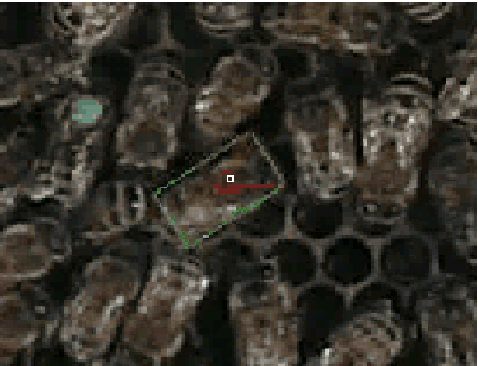
\includegraphics[width=0.23\linewidth]{changepoints/figs/app/tracker-1.png} \hspace{2em}
    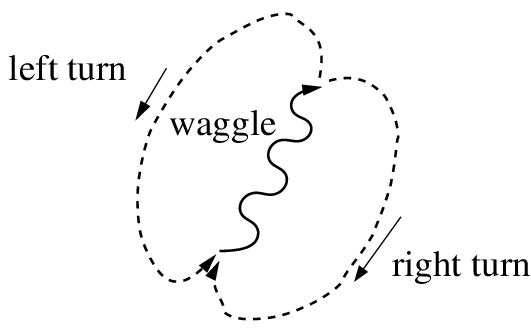
\includegraphics[width=0.27\linewidth]{changepoints/figs/app/bee_dance-1.png}
\caption{Dancer bees are tracked by a appearance based tracker from video sequences. The tracked bee is shown in green rectangle in the left figure above. The right figure shows a stylized bee dance through which bees talk to the other bees about the orientation and distance to the food sources.}
\label{fig:bees}
\end{figure}

\begin{figure}[H]
    \centering
    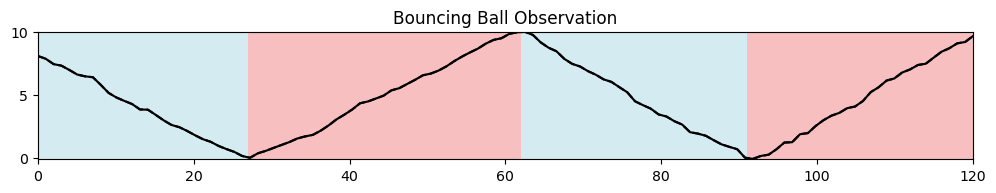
\includegraphics[width=0.85\linewidth]{changepoints/figs/ex/ex0.png}
    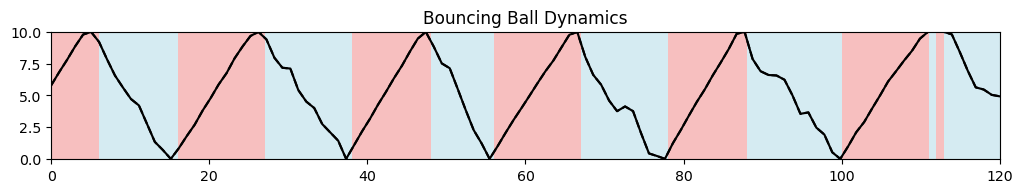
\includegraphics[width=0.85\linewidth]{changepoints/figs/ex/ex1.png}
    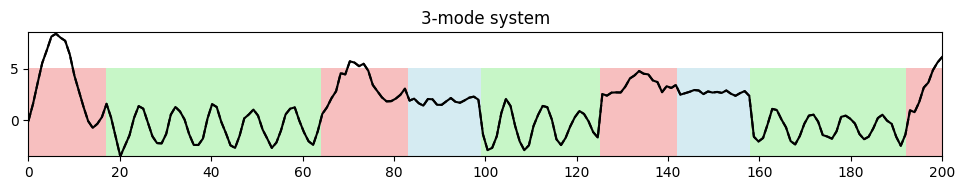
\includegraphics[width=0.85\linewidth]{changepoints/figs/ex/ex2.png}
    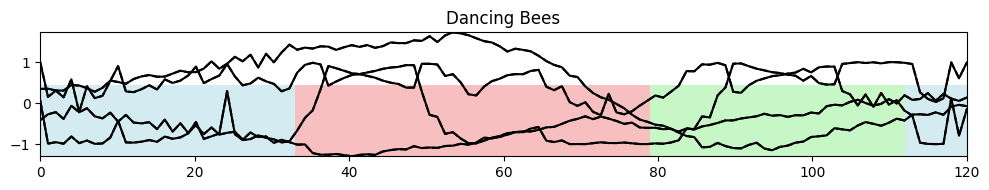
\includegraphics[width=0.85\linewidth]{changepoints/figs/ex/ex3.png}
    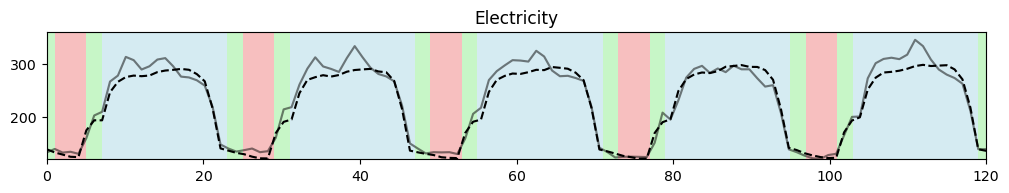
\includegraphics[width=0.85\linewidth]{changepoints/figs/ex/ex4.png}
    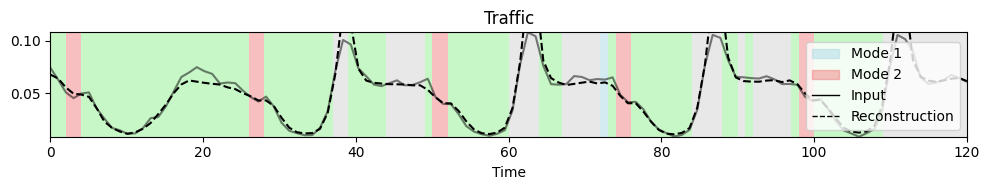
\includegraphics[width=0.85\linewidth]{changepoints/figs/ex/ex5.png}
\caption{Examples of datasets and prediction results. Dotted line represents prediction whereas solid lines represents ground truth; background colors
represent the different operating modes segmented by our base predictor RED-SDS.}
\label{fig:examples}
\end{figure}

\newpage
\subsection{Additional Experiments}
\label{app:more_experiments}

\paragraph{Additional Baselines} We add comparison to three more baselines that handles distribution shift in time series data. They are DtACI \cite{angelopoulos2024online},  ECI \cite{wu2025error}, and L-ARC \cite{zecchin2024localized}.

We would like to emphasize that these baselines are reactive. The question we try to address with CPTC is - what happens when we can anticipate distribution shift? CPTC is designed such that it greatly improves coverage compared to purely reactive methods, while still maintaining the ability to adapt to unknown shifts. To our knowledge, there are no other models that explore the same problem; CPTC provides practitioners with a simple and sound solution, when they have the ability (such as via a state space model) to predict shifts.

\begin{table}[h]
\caption{Performance on synthetic and real-world datasets with target confidence $1-\alpha = 0.9$ (for horizon $T=200$ for synthetic datasets, $300$ for electricity and traffic, and $60$ for bee, mean $\pm$ standard deviation of the test samples).  Methods that are \textit{invalid} (coverage below $90\%$) are grayed out. Our method achieves a high level of calibration (coverage is close to $90\%$) consistently. }
\vspace{1em}
\label{tab:baselines}
\centering
\resizebox{0.8\textwidth}{!}{%
\begin{tabular}{ l | c | c  c c c } 
\toprule
& & DtACI & ECI-cutoff & L-ARC & Ours \\ 
\midrule\midrule
\multirow{2}{*}{\begin{tabular}{l}Bouncing  \\ Ball obs.\end{tabular}} & Cov & \color{gray}{82.97 \plusminus 1.35}& \color{gray}{79.86 \plusminus 1.42}& \color{gray}{75.12 \plusminus 9.25} & 92.06 \plusminus 1.93\\ 
 & Width & \color{gray}{3.21 \plusminus 0.80}& \color{gray}{3.02 \plusminus 0.72}& \color{gray}{1.89 \plusminus 0.76} & 10.70 \plusminus 3.01\\ 
\midrule
\multirow{2}{*}{\begin{tabular}{l}Bouncing  \\ Ball dyn.\end{tabular}} & Cov & \color{gray}{79.63 \plusminus 1.10}& \color{gray}{80.91 \plusminus 1.28}& \color{gray}{78.63 \plusminus 6.21} & 90.62 \plusminus 3.85\\ 
 & Width & \color{gray}{3.51 \plusminus 2.20}& \color{gray}{2.32 \plusminus 0.19}& \color{gray}{2.44 \plusminus 0.23} & 10.73 \plusminus 3.67\\ 
\midrule
\multirow{2}{*}{\begin{tabular}{l}3-Mode \\ System\end{tabular}} & Cov & \color{gray}{88.82 \plusminus 0.95}& \color{gray}{83.67 \plusminus 0.89}& 92.58 \plusminus 2.77 & 90.43 \plusminus 1.92\\ 
 & Width & \color{gray}{12.55 \plusminus 7.52}& \color{gray}{2.39 \plusminus 0.48}& 12.31 \plusminus 2.85 &  4.80 \plusminus 2.64\\ 
\midrule
\midrule
\multirow{2}{*}{\begin{tabular}{l}Traffic\end{tabular}} & Cov & \color{gray}{89.14 \plusminus 0.40}& \color{gray}{86.12 \plusminus 0.50}& 90.05 \plusminus 6.24 & 92.38 \plusminus 1.24\\ 
 & Width & \color{gray}{10.35 \plusminus 9.85}& \color{gray}{7.02 \plusminus 9.72}& 8.39 \plusminus 10.13 & 15.83 \plusminus 5.96\\ 
\midrule
\multirow{2}{*}{\begin{tabular}{l}Electricity\end{tabular}} & Cov & \color{gray}{88.35 \plusminus 0.38}& \color{gray}{89.41 \plusminus 0.47}& \color{gray}{86.42 \plusminus 4.96} & 91.19 \plusminus 1.22\\ 
 & Width & \color{gray}{189.51 \plusminus 187.25}& \color{gray}{138.72 \plusminus 83.30}& \color{gray}{157.82 \plusminus 95.02} & 249.46 \plusminus 1365.46 \\ 
\midrule
\multirow{2}{*}{\begin{tabular}{l}Dancing \\ Bees\end{tabular}} & Cov & \color{gray}{78.91 \plusminus 3.02}& \color{gray}{80.12 \plusminus 2.85}& \color{gray}{75.92 \plusminus 14.21} & 95.71 \plusminus 4.95 \\
 & Width & \color{gray}{0.03 \plusminus 0.01}& \color{gray}{0.08 \plusminus 0.01}& \color{gray}{0.28 \plusminus 0.15} & 0.33 \plusminus 0.14 \\
\bottomrule
\end{tabular}
}
\end{table}

\paragraph{Longer horizon Data} Result for the same set of experiments performed on longer horizon  ($T=10,000$ for synthetic datasets amd $T=4,000$ for Electricity and Traffic datasets) is presented in table \ref{tab:baselines_long_horizon}. We added the setting where the added noise to the bouncing ball dataset is varying over the course of the time series, which is more challenging than the original settings. In the longer horizon case, both SPCI and HopCPT achieve their state of the art performance. Our method remains valid yet achieves less sharp interval width. 

\begin{table}[H]
\caption{Longer time horizon ($T=10,000$ for synthetic datasets amd $T=4,000$ for Electricity and Traffic datasets). Performance in synthetic and real-world datasets with target confidence $1-\alpha = 0.9$. Methods that are \textit{invalid} (coverage below $90\%$) are grayed out. Our method achieves a high level of calibration (coverage is close to $90\%$) consistently.} \vspace{0.5em}
\label{tab:baselines_long_horizon}
\centering
\resizebox{\textwidth}{!}{%
\begin{tabular}{ l | c | c  c c c c c }\toprule
& & RED-SDS & CP & ACI & SPCI  & HopCPT & Ours \\
\midrule\midrule
\multirow{2}{*}{\begin{tabular}{l}Bouncing Ball \\ obs.\end{tabular}} & Cov & \color{gray}{89.31 \plusminus 5.15}& \color{gray}{81.55 \plusminus 7.10} & 89.25 \plusminus 1.40 & 90.05 \plusminus 0.04 & 90.02 \plusminus 0.02 & 90.53 \plusminus 0.23\\
 & Width & \color{gray}{2.65 \plusminus 0.11}& \color{gray}{2.65 \plusminus 0.85}& 3.53 \plusminus 0.81& 1.95 \plusminus 0.12 & 1.99 \plusminus 0.08 & 2.25 \plusminus 0.54\\
\midrule
\multirow{2}{*}{\begin{tabular}{l}Bouncing Ball \\ dyn.\end{tabular}} & Cov & \color{gray}{45.12 \plusminus 25.50}& \color{gray}{42.88 \plusminus 6.95}& \color{gray}{87.95 \plusminus 1.05}& 90.04 \plusminus 0.04 & 90.01 \plusminus 0.04 & 90.05 \plusminus 0.04\\
 & Width & \color{gray}{1.67 \plusminus 0.13}& \color{gray}{0.95 \plusminus 0.51}& \color{gray}{3.10 \plusminus 1.04}& 3.24  \plusminus 0.14 & 3.07 \plusminus 0.10 & 3.18 \plusminus 0.91\\
\midrule
\multirow{2}{*}{\begin{tabular}{l}3-Mode \\ System\end{tabular}} & Cov & \color{gray}{68.52 \plusminus 3.53}& \color{gray}{65.24 \plusminus 5.51}& 89.75 \plusminus 0.90& 90.05 \plusminus 0.02 & 90.02 \plusminus 0.04 & 90.08 \plusminus 0.05\\
 & Width & \color{gray}{2.56 \plusminus 0.21}& \color{gray}{2.33 \plusminus 0.63}& 3.74 \plusminus 0.61& 2.67 \plusminus 0.94 & 2.49 \plusminus 1.31 &  3.12 \plusminus 2.63\\
\midrule
\midrule
\multirow{2}{*}{\begin{tabular}{l}Bouncing Ball \\ obs. varying\end{tabular}} & Cov & \color{gray}{60.83 \plusminus 22.53}& \color{gray}{40.25 \plusminus 6.52}& 88.60 \plusminus 1.25& 90.02 \plusminus 0.04 & 90.04 \plusminus 0.00 & 90.10 \plusminus 0.03\\
 & Width & \color{gray}{2.10 \plusminus 0.45}& \color{gray}{1.73 \plusminus 0.91}& 3.70 \plusminus 0.95 & 2.11 \plusminus 0.82 & 2.14 \plusminus 0.73 & 2.41 \plusminus 1.22\\
\midrule
\multirow{2}{*}{\begin{tabular}{l}Bouncing Ball \\ dyn. varying\end{tabular}} & Cov & \color{gray}{44.25 \plusminus 26.11}& \color{gray}{41.73 \plusminus 7.12}& \color{gray}{88.05 \plusminus 1.00}& 90.05 \plusminus 0.03 & 90.02 \plusminus 0.04 & 90.08 \plusminus 0.03\\
 & Width & \color{gray}{1.85 \plusminus 0.12}& \color{gray}{0.92 \plusminus 0.55}& \color{gray}{3.13 \plusminus 1.14}& 2.92 \plusminus 0.21 & 3.05 \plusminus 0.19 & 3.40 \plusminus 0.32\\
\midrule
\midrule
\multirow{2}{*}{\begin{tabular}{l}Traffic\end{tabular}} & Cov & \color{gray}{87.14 \plusminus 10.51}& \color{gray}{70.52 \plusminus 2.83}& \color{gray}{89.15 \plusminus 0.38}& 90.01 \plusminus 0.04 & 90.03 \plusminus 0.03 & 90.02 \plusminus 0.03\\
 & Width & \color{gray}{2.91 \plusminus 1.62}& \color{gray}{0.43 \plusminus 0.25}& \color{gray}{55.10 \plusminus 24.13}& 4.81 \plusminus 2.42 & 7.84 \plusminus 10.53 & 8.55 \plusminus 14.11\\
\midrule
\multirow{2}{*}{\begin{tabular}{l}Electricity\end{tabular}} & Cov & \color{gray}{76.10 \plusminus 13.52}& \color{gray}{69.53 \plusminus 3.21}& \color{gray}{89.05 \plusminus 0.33}& 90.02 \plusminus 0.03 & 90.00 \plusminus 0.02 & 90.43 \plusminus 0.03\\
 & Width & \color{gray}{91.30 \plusminus 125.10}& \color{gray}{62.10 \plusminus 451.20}& \color{gray}{31.40 \plusminus 171.30}& 162.02 \plusminus 11.40 & 161.70 \plusminus 15.20 & 173.38 \plusminus 31.10 \\
\bottomrule
\end{tabular}
}
\end{table}

\paragraph{Aggregation methods.} In this study we compare the two different aggregation methods. First is the case where we chose the minimum size, i.e. $\Gamma_t(x_t) = $ \Eqref{eq:aggregation-average}. Algorithmically, we discretize the output space $\mathcal{Y}$ into intervals of length 0.02, and calculate probability mass for each interval. We refer to this method as \emph{min}. Aggregation by union numbers (the same as in the main text using \Eqref{eq:aggregation-union}) are referred to as \emph{union}. Results are present in table \ref{tab:aggregation} where the performance are very similar. When there are two modes (bouncing ball cases) the prediction intervals are almost identical.
 
\begin{table}[h!]
\centering
\caption{Ablation Study on two different Union (\textit{union}, \eqref{eq:aggregation-union}) and grid-discretization (\textit{min}, \eqref{eq:aggregation-average}).}
\vspace{0.5em}
\label{tab:aggregation}
\begin{tabular}{lcccccc}
\toprule
& BB obs. & BB dyn. & 3-mode system & traffic & electricity & bees \\
\midrule
\midrule
Coverage (\textit{union}) & 90.53 & 90.44 & 93.35 & 92.76 & 92.62 & 93.43 \\
Coverage (\emph{min})  & 90.03 & 90.32 & 91.50 & 91.87 & 89.82 & 90.28 \\
Width (\textit{union})   & 3.73  & 1.72  & 2.45 & 7.94  & 166.88 & 0.79 \\
Width (\emph{min})     & 3.62 & 1.65  & 2.41 & 7.95  & 153.57 & 0.77 \\
\bottomrule
\end{tabular}
\end{table}

\paragraph{Discussion on Misspecified Regimes.} We designed the number of latent states to be a hyperparameter given by the user. Our method ensures that the validity guarantee still holds even if the state cardinality is incorrect (theorem 4.2), as incorrect state cardinality can be formulated as a case of incorrect classification. Determining state space cardinality is a well-studied problem (see for example \cite{branicky1994stability}), and we consider it to be beyond the scope of our paper.

Regarding the effect on performance, our ablation studies (Section 5.2, Tables \ref{tab:z_exp} and \ref{tab:z_exp_area}) demonstrate that while the validity (coverage) of CPTC is robust to errors in state prediction, the sharpness (width of prediction intervals) can be affected. Table 3 explicitly shows that "the more accurate the state prediction is, the sharper the intervals." This implies that selecting a more appropriate number of regimes that better captures the true underlying dynamics would lead to narrower and more efficient prediction intervals.

\subsection{Qualitative Results}
\label{app:pictures}

We provide additional visualizations to present qualitative comparisons of CPTC compared to baseline models. Figures \ref{fig:synthetic}, \ref{fig:pic2}, and \ref{fig:pic3} show consistent results with the analysis in section 5, where CPTC shows stronger adaptivity and validity for uncertainty quantification in time series with these nonstationary dynamics.



\begin{figure}[h!]
    \centering
    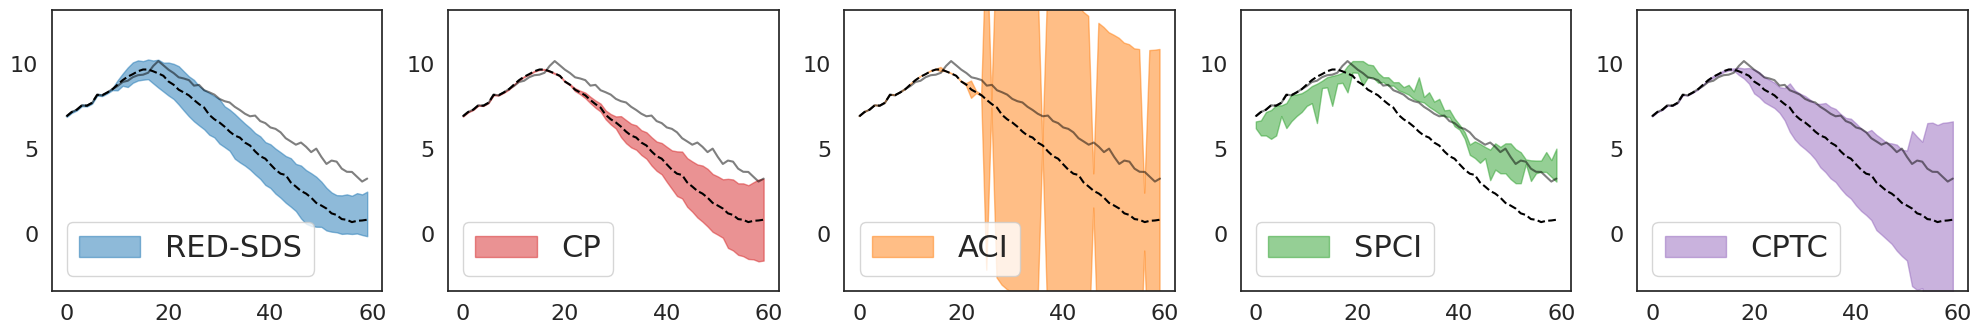
\includegraphics[width=\linewidth]{changepoints/figs/ex/a.png}
    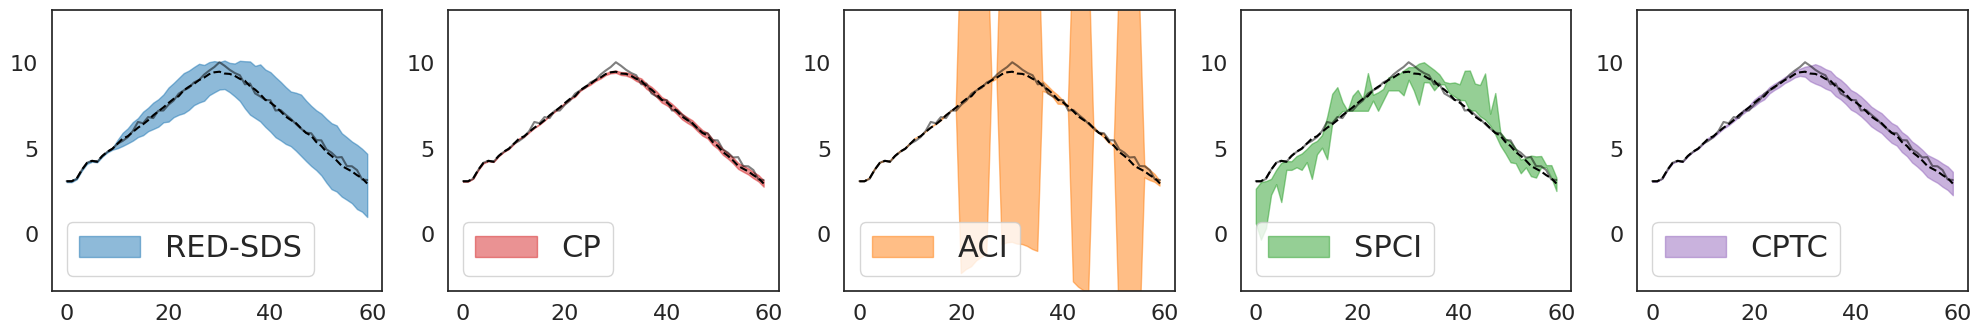
\includegraphics[width=\linewidth]{changepoints/figs/ex/b.png}
    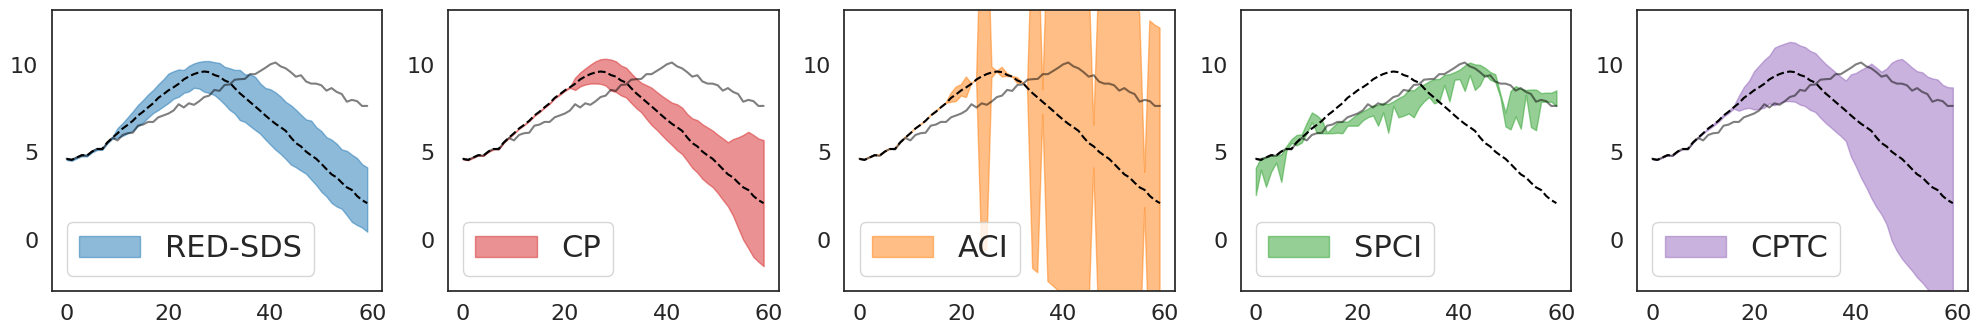
\includegraphics[width=\linewidth]{changepoints/figs/ex/c.png}
    \caption{\textbf{Qualitative comparison of the prediction interval on the bouncing ball w/ dynamics noise dataset.} The dashed line is the predicted state whereas the solid gray line is the observation. We see that our CPTC algorithm can increase the interval in anticipation of an uncertain state change (top panel), is stabler when the prediction is accuracy compared to ACI and SPCI (middle panel), and is adaptive to inaccurate predictions (botom panel).}
    \label{fig:synthetic}
     %\vspace{-0.5em}
\end{figure}


% \begin{figure}[H]
%     \centering
%     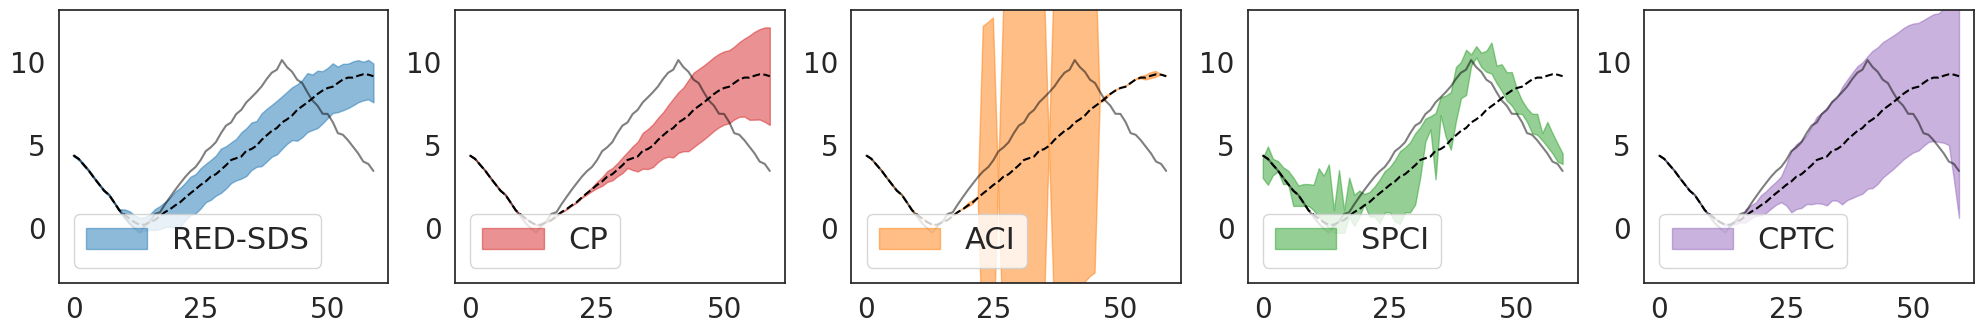
\includegraphics[width=\linewidth]{changepoints/figs/app/a1.png}
%     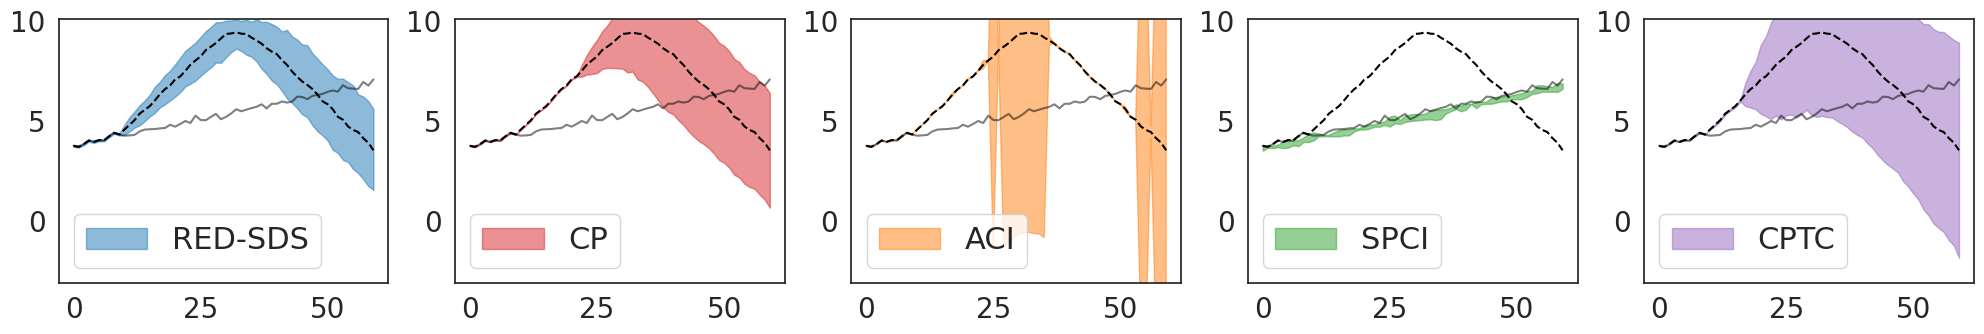
\includegraphics[width=\linewidth]{changepoints/figs/app/a2.png}
%     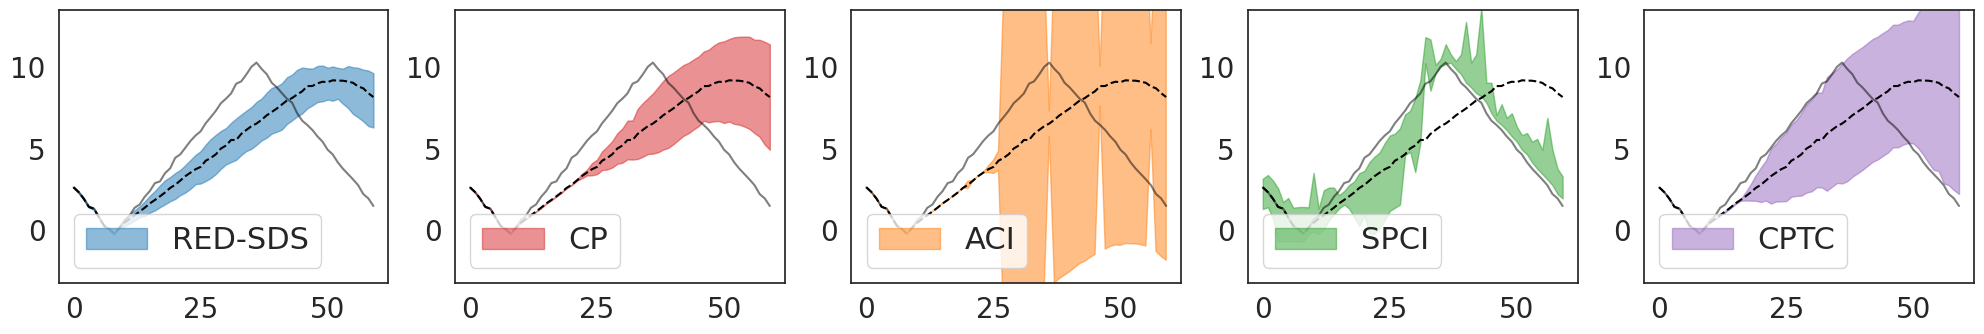
\includegraphics[width=\linewidth]{changepoints/figs/app/a3.png}
%     \caption{Visualization of prediction intervals on the Bouncing Ball Obs dataset.}
%     \label{fig:pic1}
%     \vspace{-1em}
% \end{figure}
\vspace{-1em}
\begin{figure}[H]
    \centering
    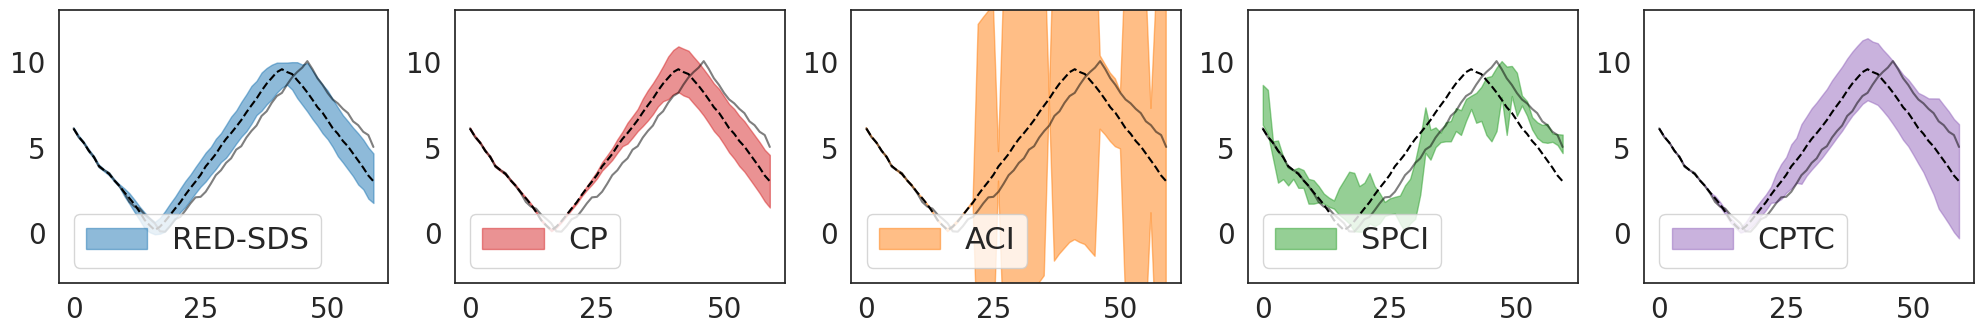
\includegraphics[width=\linewidth]{changepoints/figs/app/b1.png}
    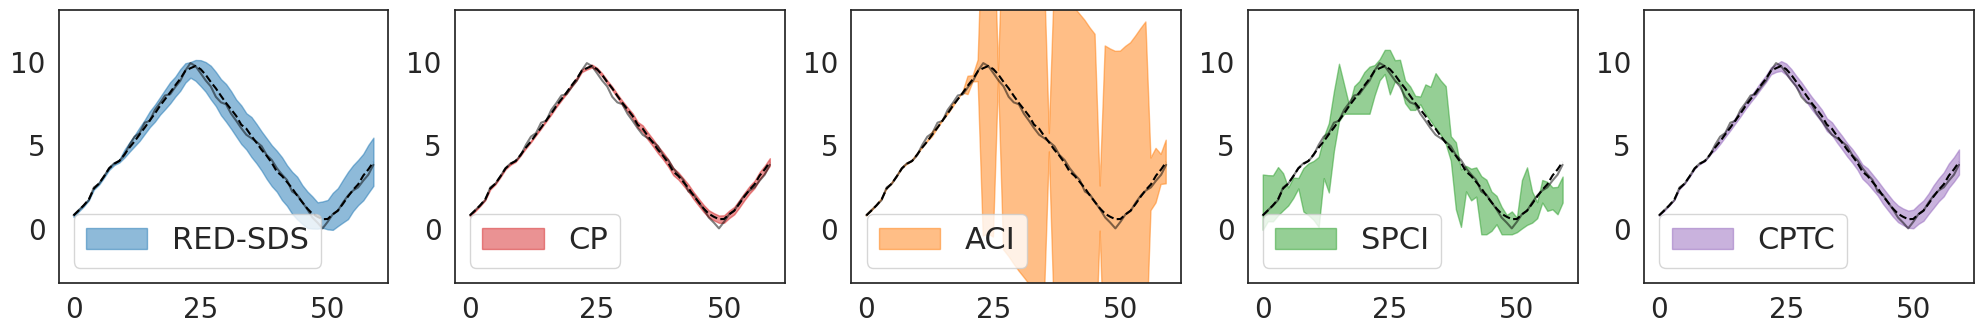
\includegraphics[width=\linewidth]{changepoints/figs/app/b2.png}
    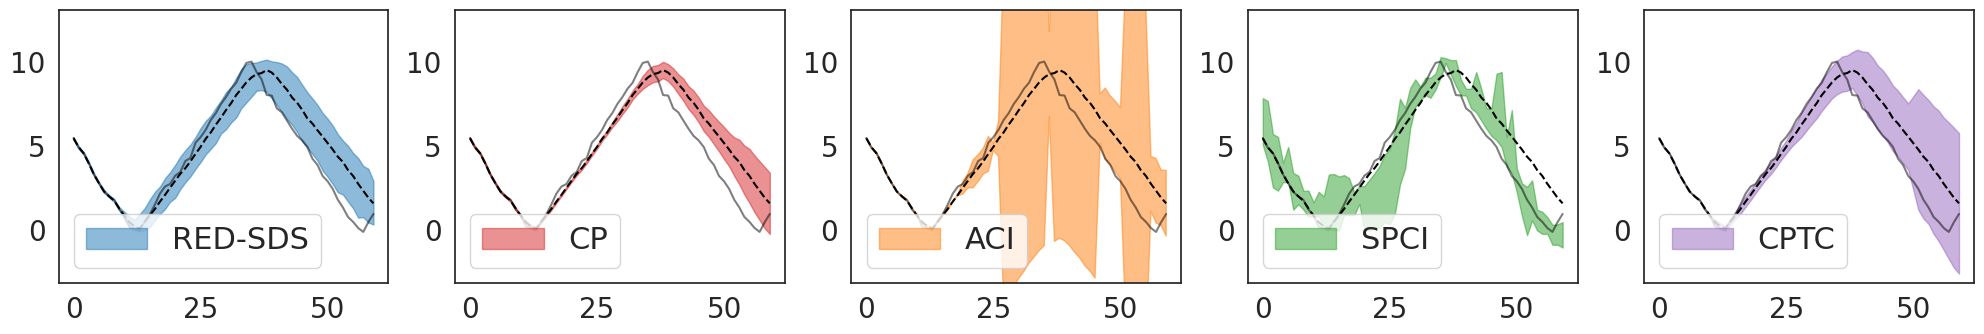
\includegraphics[width=\linewidth]{changepoints/figs/app/b3.png}
    \caption{Visualization of prediction intervals on the Bouncing Ball Obs dataset.}
    \label{fig:pic2}
\end{figure}
\vspace{2em}

\begin{figure}[H]
    \centering
    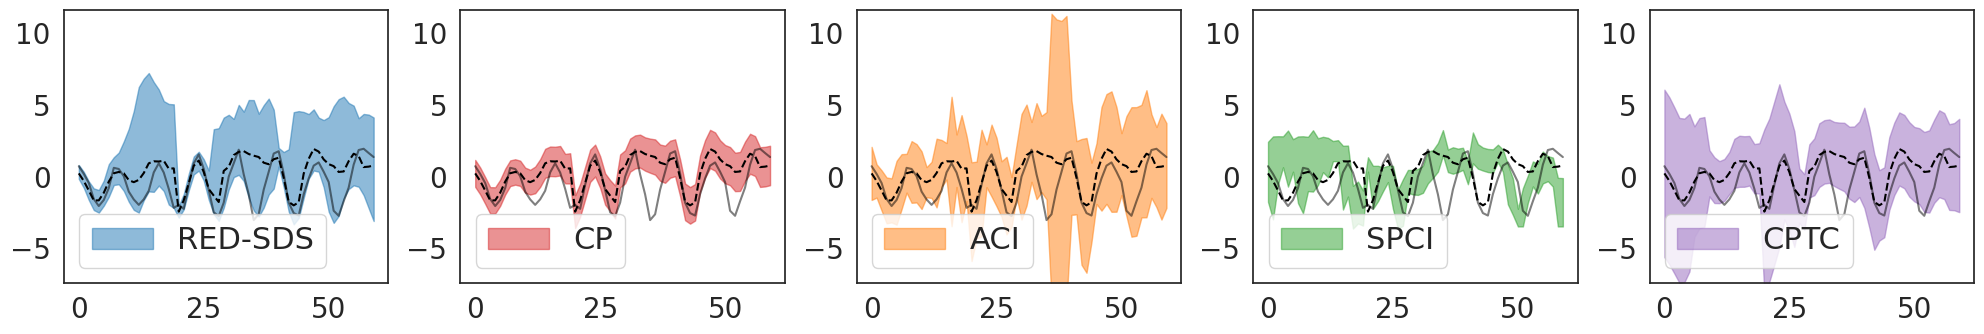
\includegraphics[width=\linewidth]{changepoints/figs/app/c1.png}
    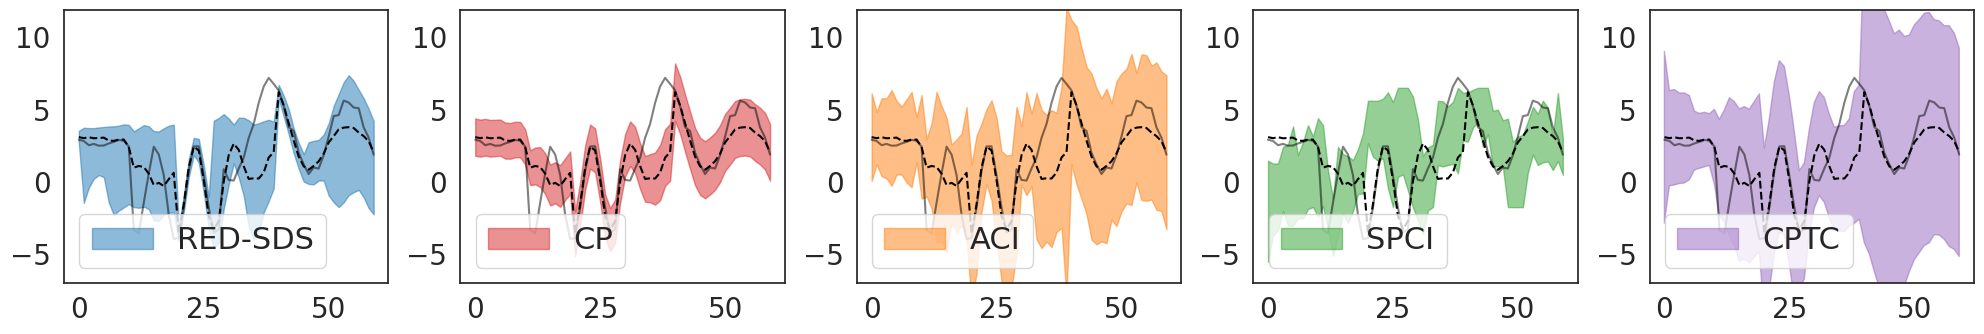
\includegraphics[width=\linewidth]{changepoints/figs/app/c2.png}
    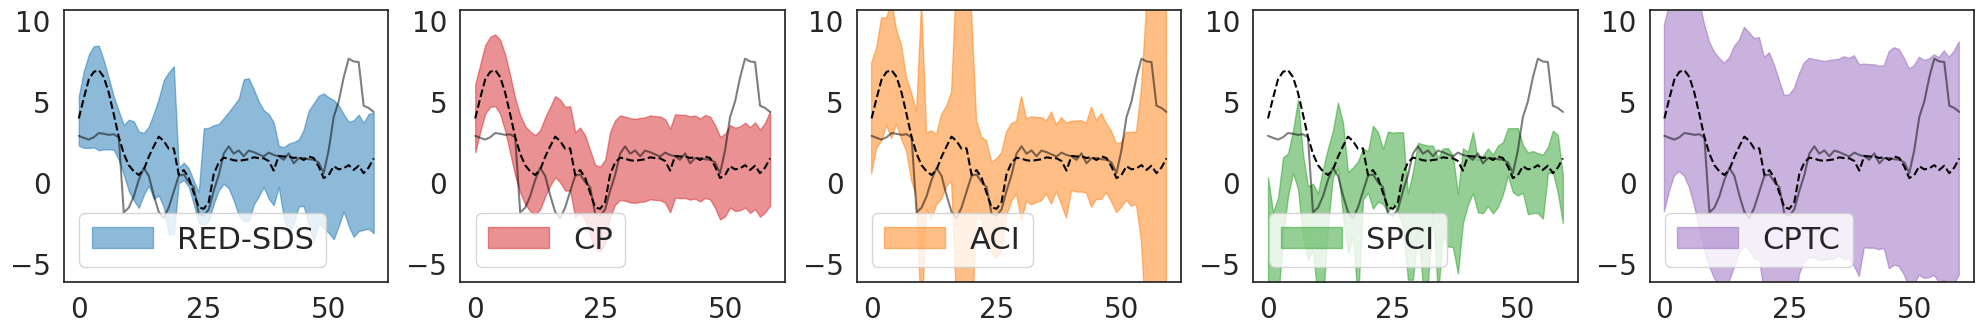
\includegraphics[width=\linewidth]{changepoints/figs/app/c3.png}
    \caption{Visualization of prediction intervals on the 3 mode system datasets.}
    \label{fig:pic3}
\end{figure}

\section{Runtime analysis}

We provide a runtime analysis comparing the aggregation methods in Equations \ref{eq:aggregation-average} and \ref{eq:aggregation-union} and with baselines.

\textbf{Notation}

\begin{itemize}
    \item $T$: Total timesteps, $K$: Number of states, $M$: State prediction model inference complexity
    \item Score sets $\mathcal{S}_z$ maintained in sorted order (quantile computation in $\mathcal{O}(1)$, insertion $\mathcal{O}(\log T)$)
\end{itemize}

\textbf{Complexity Per Timestep}

\begin{enumerate}
    \item Computing quantile $Q^{1-\alpha_t}(\mathcal{S}_z^{(l)})$ for each state, totaling $\mathcal{O}(K)$.
    \item State Prediction: computing $\hat{p}(z_t|x_t)$ and sampling a state, totaling $\mathcal{O}(M)$.
    \item Aggregation
    \begin{itemize}
        \item \textit{Eq. 10, Weighted Level-Set:} $\mathcal{O}(K \cdot \lceil 1/\delta \rceil^d)$ where $\delta$ is discretization resolution
        \item \textit{Eq. 11, Union:} $\mathcal{O}(K \log K)$ for sorting states by probability
    \end{itemize}
    \item Updates: $\mathcal{O}(\log t)$ for inserting new score into sorted set.
\end{enumerate}

\textit{Therefore, the total complexity of CPTC with horizon $T$ is:}

$\mathcal{O}(T \cdot (M + K \cdot \lceil \frac{1}{\delta} \rceil^d) + T \log T)$ if we use the Weighted Level-Set as aggregation in Eq. 10, and

$\mathcal{O}(T \cdot (M + K \log K) + T \log T)$ if we use the more efficient Union aggregation in Eq. 11.

In practice, both $M$ (inference cost) and $K$ (number of discrete states) are small. For applications where $K = \mathcal{O}(1)$ and $M = \mathcal{O}(1)$, CPTC achieves near-linear scaling $\mathcal{O}(T \log T)$, the same as ACI (see table below).

If we use the more precise weighted level set aggregation method, the runtime largely depends on the discretization resolution $\delta$, output dimension $d$, and the number of states $K$. We remark the level set approach scales poorly if the resolution, dimension, or number of states are high.

\begin{table}[h]
\centering
\begin{tabular}{lll}
\hline
\textbf{Method} & \textbf{Time Complexity} & \textbf{Remarks} \\
\hline
ACI & $\mathcal{O}(T \log T)$ & Single score set, no state awareness \\
SPCI / HopCPT & $\mathcal{O}(T^2 \log T)$ & Re-train regression model at every time step \\
CPTC (Union) & $\mathcal{O}(T \log T)$ & State-aware, pre-trained predictor \\
\hline
\end{tabular}
\end{table}
% \subsection{Ablation study on non state-dependent forecaster}

% We can still use CPTC when we only have one forecaster but have access to some state prediction (for example in the form of external parameters). We can apply algorithm \ref{alg:cptc} directly with the special case where $\hat{f}(x,z_i) = \hat{f}(x,z_j)$ for any $x \in \gX and z_i, z_j \in \gZ$. Table \ref{tab:one_forecaster} presents the performance of the algorithm in this case.

% \begin{table}[]
% \caption{One forecaster} %\vspace{-0.5em}
% \label{tab:one_forecaster}
% \centering
% \begin{tabular}{ l | c | c  c } 
% \toprule
% & & SPCI  & Ours \\
% \midrule\midrule
% \multirow{2}{*}{\begin{tabular}{l}Bouncing Ball \\ obs.\end{tabular}} & Cov & \color{gray}{37.90 \plusminus 9.78} & 92.16 \plusminus 26.88\\ 
%  & Width & \color{gray}{1.45 \plusminus 0.85} & 7.43 \plusminus 4.68\\ 
% \midrule
% \multirow{2}{*}{\begin{tabular}{l}Bouncing Ball \\ dyn.\end{tabular}} & Cov & \color{gray}{53.62 \plusminus 7.75} & 90.58 \plusminus 29.21\\ 
%  & Width & \color{gray}{2.02 \plusminus 0.23} & 8.11 \plusminus 4.93\\ 
% \midrule
% \multirow{2}{*}{\begin{tabular}{l}3-Mode \\ System\end{tabular}} & Cov & \color{gray}{81.72 \plusminus 2.88} & 93.35 \plusminus 3.51\\ 
%  & Width & \color{gray}{3.94 \plusminus 0.85} & 13.68 \plusminus 2.49\\ 
% \midrule\midrule
% \multirow{2}{*}{\begin{tabular}{l}Traffic\end{tabular}} & Cov & \color{gray}{88.24 \plusminus 2.13} & 94.76 \plusminus 4.93\\ 
%  & Width & \color{gray}{4.62 \plusminus 2.28} & 8.34 \plusminus 14.44\\ 
% \midrule
% \multirow{2}{*}{\begin{tabular}{l}Electricity\end{tabular}} & Cov & \color{gray}{86.62 \plusminus 2.97} & 93.82 \plusminus 4.22\\ 
%  & Width & \color{gray}{371.69 \plusminus 305.86} & 98.87 \plusminus 49.35\\ 
% \midrule
% \multirow{2}{*}{\begin{tabular}{l}Dancing Bees\end{tabular}} & Cov & \color{gray}{79.2 \plusminus 0.3} & 93.43 \plusminus 11.42 \\
%  & Width & \color{gray}{1.77 \plusminus 1.38} & 1.15 \plusminus 0.56 \\
% \bottomrule
% \end{tabular}
% \end{table}



% \subsection{Experiment on state prediction (continued) }
% \label{app:z_exp}

% \begin{table*}[h!]
%     \centering
%     \begin{tabular}{c|c c c c}
%         \hline
%         \toprule
%         $T=250$& Ground truth state labels & GT w/ $20\%$ error & GT w/ $50\%$ error & Learned state labels \\ 
%         \midrule
%         BB obs. noise & 90.00 \plusminus 0.32 & 89.94 \plusminus 0.29 & 89.92 \plusminus 0.28 & 89.11 \plusminus 3.54 \\ 
%         BB dyn. noise & 90.04 \plusminus 0.34 & 90.01 \plusminus 0.35 & 89.96 \plusminus 0.30 & 90.11 \plusminus 0.33\\ 
%         3-mode system & 89.34 \plusminus 0.87 &  89.40 \plusminus 0.91  & 89.64 \plusminus 0.80 & 89.72 \plusminus 1.51 \\ 
%         \midrule\midrule
%         $T=1000$& Ground truth state labels & GT w/ $20\%$ error & GT w/ $50\%$ error & Learned state labels \\ 
%         \midrule
%         BB obs. noise & 90.00 \plusminus 0.32 & 89.94 \plusminus 0.29 & 89.92 \plusminus 0.28 & 89.11 \plusminus 3.54 \\ 
%         BB dyn. noise & 90.04 \plusminus 0.34 & 90.01 \plusminus 0.35 & 89.96 \plusminus 0.30 & 90.11 \plusminus 0.33\\ 
%         3-mode system & 89.34 \plusminus 0.87 &  89.40 \plusminus 0.91  & 89.64 \plusminus 0.80 & 89.72 \plusminus 1.51 \\ 
%         \bottomrule
%     \end{tabular}
%     \caption{Coverage of CPTC for using ground truth (GT) labels, GT labels with injected noise, and learned  label predictions on synthetic data with $T=250, 1000$. We can see that coverage performance does not change significantly with error in state prediction. }
%     \label{tab:z_exp_small}
% \end{table*}

% 
\newpage
\section*{NeurIPS Paper Checklist}

% %%% BEGIN INSTRUCTIONS %%%
% The checklist is designed to encourage best practices for responsible machine learning research, addressing issues of reproducibility, transparency, research ethics, and societal impact. Do not remove the checklist: {\bf The papers not including the checklist will be desk rejected.} The checklist should follow the references and follow the (optional) supplemental material.  The checklist does NOT count towards the page
% limit. 

% Please read the checklist guidelines carefully for information on how to answer these questions. For each question in the checklist:
% \begin{itemize}
%     \item You should answer \answerYes{}, \answerNo{}, or \answerNA{}.
%     \item \answerNA{} means either that the question is Not Applicable for that particular paper or the relevant information is Not Available.
%     \item Please provide a short (1–2 sentence) justification right after your answer (even for NA). 
%    % \item {\bf The papers not including the checklist will be desk rejected.}
% \end{itemize}

% {\bf The checklist answers are an integral part of your paper submission.} They are visible to the reviewers, area chairs, senior area chairs, and ethics reviewers. You will be asked to also include it (after eventual revisions) with the final version of your paper, and its final version will be published with the paper.

% The reviewers of your paper will be asked to use the checklist as one of the factors in their evaluation. While "\answerYes{}" is generally preferable to "\answerNo{}", it is perfectly acceptable to answer "\answerNo{}" provided a proper justification is given (e.g., "error bars are not reported because it would be too computationally expensive" or "we were unable to find the license for the dataset we used"). In general, answering "\answerNo{}" or "\answerNA{}" is not grounds for rejection. While the questions are phrased in a binary way, we acknowledge that the true answer is often more nuanced, so please just use your best judgment and write a justification to elaborate. All supporting evidence can appear either in the main paper or the supplemental material, provided in appendix. If you answer \answerYes{} to a question, in the justification please point to the section(s) where related material for the question can be found.

% IMPORTANT, please:
% \begin{itemize}
%     \item {\bf Delete this instruction block, but keep the section heading ``NeurIPS Paper Checklist"},
%     \item  {\bf Keep the checklist subsection headings, questions/answers and guidelines below.}
%     \item {\bf Do not modify the questions and only use the provided macros for your answers}.
% \end{itemize} 
 

%%% END INSTRUCTIONS %%%


\begin{enumerate}

\item {\bf Claims}
    \item[] Question: Do the main claims made in the abstract and introduction accurately reflect the paper's contributions and scope?
    \item[] Answer: \answerYes{} % Replace by \answerYes{}, \answerNo{}, or \answerNA{}.
    \item[] Justification: Main content and contributions are introduced in the abstract and introduction
    \item[] Guidelines:
    \begin{itemize}
        \item The answer NA means that the abstract and introduction do not include the claims made in the paper.
        \item The abstract and/or introduction should clearly state the claims made, including the contributions made in the paper and important assumptions and limitations. A No or NA answer to this question will not be perceived well by the reviewers. 
        \item The claims made should match theoretical and experimental results, and reflect how much the results can be expected to generalize to other settings. 
        \item It is fine to include aspirational goals as motivation as long as it is clear that these goals are not attained by the paper. 
    \end{itemize}

\item {\bf Limitations}
    \item[] Question: Does the paper discuss the limitations of the work performed by the authors?
    \item[] Answer: \answerYes{} % Replace by \answerYes{}, \answerNo{}, or \answerNA{}.
    \item[] Justification: Limitations are discussed in the discussion section.
    \item[] Guidelines:
    \begin{itemize}
        \item The answer NA means that the paper has no limitation while the answer No means that the paper has limitations, but those are not discussed in the paper. 
        \item The authors are encouraged to create a separate "Limitations" section in their paper.
        \item The paper should point out any strong assumptions and how robust the results are to violations of these assumptions (e.g., independence assumptions, noiseless settings, model well-specification, asymptotic approximations only holding locally). The authors should reflect on how these assumptions might be violated in practice and what the implications would be.
        \item The authors should reflect on the scope of the claims made, e.g., if the approach was only tested on a few datasets or with a few runs. In general, empirical results often depend on implicit assumptions, which should be articulated.
        \item The authors should reflect on the factors that influence the performance of the approach. For example, a facial recognition algorithm may perform poorly when image resolution is low or images are taken in low lighting. Or a speech-to-text system might not be used reliably to provide closed captions for online lectures because it fails to handle technical jargon.
        \item The authors should discuss the computational efficiency of the proposed algorithms and how they scale with dataset size.
        \item If applicable, the authors should discuss possible limitations of their approach to address problems of privacy and fairness.
        \item While the authors might fear that complete honesty about limitations might be used by reviewers as grounds for rejection, a worse outcome might be that reviewers discover limitations that aren't acknowledged in the paper. The authors should use their best judgment and recognize that individual actions in favor of transparency play an important role in developing norms that preserve the integrity of the community. Reviewers will be specifically instructed to not penalize honesty concerning limitations.
    \end{itemize}

\item {\bf Theory assumptions and proofs}
    \item[] Question: For each theoretical result, does the paper provide the full set of assumptions and a complete (and correct) proof?
    \item[] Answer: \answerYes{} % Replace by \answerYes{}, \answerNo{}, or \answerNA{}.
    \item[] Justification: I have verified the theoretical claims tp be correct as best of my knowledge.
    \item[] Guidelines:
    \begin{itemize}
        \item The answer NA means that the paper does not include theoretical results. 
        \item All the theorems, formulas, and proofs in the paper should be numbered and cross-referenced.
        \item All assumptions should be clearly stated or referenced in the statement of any theorems.
        \item The proofs can either appear in the main paper or the supplemental material, but if they appear in the supplemental material, the authors are encouraged to provide a short proof sketch to provide intuition. 
        \item Inversely, any informal proof provided in the core of the paper should be complemented by formal proofs provided in appendix or supplemental material.
        \item Theorems and Lemmas that the proof relies upon should be properly referenced. 
    \end{itemize}

    \item {\bf Experimental result reproducibility}
    \item[] Question: Does the paper fully disclose all the information needed to reproduce the main experimental results of the paper to the extent that it affects the main claims and/or conclusions of the paper (regardless of whether the code and data are provided or not)?
    \item[] Answer: \answerYes{} % Replace by \answerYes{}, \answerNo{}, or \answerNA{}.
    \item[] Justification: Code to reproduce our results are attached in the supplementary materials. If the paper is published, we will open source the code and code for baseline models. 
    \item[] Guidelines:
    \begin{itemize}
        \item The answer NA means that the paper does not include experiments.
        \item If the paper includes experiments, a No answer to this question will not be perceived well by the reviewers: Making the paper reproducible is important, regardless of whether the code and data are provided or not.
        \item If the contribution is a dataset and/or model, the authors should describe the steps taken to make their results reproducible or verifiable. 
        \item Depending on the contribution, reproducibility can be accomplished in various ways. For example, if the contribution is a novel architecture, describing the architecture fully might suffice, or if the contribution is a specific model and empirical evaluation, it may be necessary to either make it possible for others to replicate the model with the same dataset, or provide access to the model. In general. releasing code and data is often one good way to accomplish this, but reproducibility can also be provided via detailed instructions for how to replicate the results, access to a hosted model (e.g., in the case of a large language model), releasing of a model checkpoint, or other means that are appropriate to the research performed.
        \item While NeurIPS does not require releasing code, the conference does require all submissions to provide some reasonable avenue for reproducibility, which may depend on the nature of the contribution. For example
        \begin{enumerate}
            \item If the contribution is primarily a new algorithm, the paper should make it clear how to reproduce that algorithm.
            \item If the contribution is primarily a new model architecture, the paper should describe the architecture clearly and fully.
            \item If the contribution is a new model (e.g., a large language model), then there should either be a way to access this model for reproducing the results or a way to reproduce the model (e.g., with an open-source dataset or instructions for how to construct the dataset).
            \item We recognize that reproducibility may be tricky in some cases, in which case authors are welcome to describe the particular way they provide for reproducibility. In the case of closed-source models, it may be that access to the model is limited in some way (e.g., to registered users), but it should be possible for other researchers to have some path to reproducing or verifying the results.
        \end{enumerate}
    \end{itemize}


\item {\bf Open access to data and code}
    \item[] Question: Does the paper provide open access to the data and code, with sufficient instructions to faithfully reproduce the main experimental results, as described in supplemental material?
    \item[] Answer: \answerYes{} % Replace by \answerYes{}, \answerNo{}, or \answerNA{}.
    \item[] Justification: All data and baselines used are open access. We will open open source our code as well. 
    \item[] Guidelines:
    \begin{itemize}
        \item The answer NA means that paper does not include experiments requiring code.
        \item Please see the NeurIPS code and data submission guidelines (\url{https://nips.cc/public/guides/CodeSubmissionPolicy}) for more details.
        \item While we encourage the release of code and data, we understand that this might not be possible, so “No” is an acceptable answer. Papers cannot be rejected simply for not including code, unless this is central to the contribution (e.g., for a new open-source benchmark).
        \item The instructions should contain the exact command and environment needed to run to reproduce the results. See the NeurIPS code and data submission guidelines (\url{https://nips.cc/public/guides/CodeSubmissionPolicy}) for more details.
        \item The authors should provide instructions on data access and preparation, including how to access the raw data, preprocessed data, intermediate data, and generated data, etc.
        \item The authors should provide scripts to reproduce all experimental results for the new proposed method and baselines. If only a subset of experiments are reproducible, they should state which ones are omitted from the script and why.
        \item At submission time, to preserve anonymity, the authors should release anonymized versions (if applicable).
        \item Providing as much information as possible in supplemental material (appended to the paper) is recommended, but including URLs to data and code is permitted.
    \end{itemize}


\item {\bf Experimental setting/details}
    \item[] Question: Does the paper specify all the training and test details (e.g., data splits, hyperparameters, how they were chosen, type of optimizer, etc.) necessary to understand the results?
    \item[] Answer: \answerYes{} % Replace by \answerYes{}, \answerNo{}, or \answerNA{}.
    \item[] Justification: Important information discussed in the experiments section, and details are in the appendix. 
    \item[] Guidelines:
    \begin{itemize}
        \item The answer NA means that the paper does not include experiments.
        \item The experimental setting should be presented in the core of the paper to a level of detail that is necessary to appreciate the results and make sense of them.
        \item The full details can be provided either with the code, in appendix, or as supplemental material.
    \end{itemize}

\item {\bf Experiment statistical significance}
    \item[] Question: Does the paper report error bars suitably and correctly defined or other appropriate information about the statistical significance of the experiments?
    \item[] Answer: \answerYes{} % Replace by \answerYes{}, \answerNo{}, or \answerNA{}.
    \item[] Justification: included error bars.
    \item[] Guidelines:
    \begin{itemize}
        \item The answer NA means that the paper does not include experiments.
        \item The authors should answer "Yes" if the results are accompanied by error bars, confidence intervals, or statistical significance tests, at least for the experiments that support the main claims of the paper.
        \item The factors of variability that the error bars are capturing should be clearly stated (for example, train/test split, initialization, random drawing of some parameter, or overall run with given experimental conditions).
        \item The method for calculating the error bars should be explained (closed form formula, call to a library function, bootstrap, etc.)
        \item The assumptions made should be given (e.g., Normally distributed errors).
        \item It should be clear whether the error bar is the standard deviation or the standard error of the mean.
        \item It is OK to report 1-sigma error bars, but one should state it. The authors should preferably report a 2-sigma error bar than state that they have a 96\% CI, if the hypothesis of Normality of errors is not verified.
        \item For asymmetric distributions, the authors should be careful not to show in tables or figures symmetric error bars that would yield results that are out of range (e.g. negative error rates).
        \item If error bars are reported in tables or plots, The authors should explain in the text how they were calculated and reference the corresponding figures or tables in the text.
    \end{itemize}

\item {\bf Experiments compute resources}
    \item[] Question: For each experiment, does the paper provide sufficient information on the computer resources (type of compute workers, memory, time of execution) needed to reproduce the experiments?
    \item[] Answer: \answerYes{}% Replace by \answerYes{}, \answerNo{}, or \answerNA{}.
    \item[] Justification: Described in detail in appendix B.
    \item[] Guidelines:
    \begin{itemize}
        \item The answer NA means that the paper does not include experiments.
        \item The paper should indicate the type of compute workers CPU or GPU, internal cluster, or cloud provider, including relevant memory and storage.
        \item The paper should provide the amount of compute required for each of the individual experimental runs as well as estimate the total compute. 
        \item The paper should disclose whether the full research project required more compute than the experiments reported in the paper (e.g., preliminary or failed experiments that didn't make it into the paper). 
    \end{itemize}
    
\item {\bf Code of ethics}
    \item[] Question: Does the research conducted in the paper conform, in every respect, with the NeurIPS Code of Ethics \url{https://neurips.cc/public/EthicsGuidelines}?
    \item[] Answer:\answerYes{} % Replace by \answerYes{}, \answerNo{}, or \answerNA{}.
    \item[] Justification: We followed the code of ethics.
    \item[] Guidelines:
    \begin{itemize}
        \item The answer NA means that the authors have not reviewed the NeurIPS Code of Ethics.
        \item If the authors answer No, they should explain the special circumstances that require a deviation from the Code of Ethics.
        \item The authors should make sure to preserve anonymity (e.g., if there is a special consideration due to laws or regulations in their jurisdiction).
    \end{itemize}


\item {\bf Broader impacts}
    \item[] Question: Does the paper discuss both potential positive societal impacts and negative societal impacts of the work performed?
    \item[] Answer: \answerYes{} % Replace by \answerYes{}, \answerNo{}, or \answerNA{}.
    \item[] Justification: Addressed positive impacts but not negative ones.
    \item[] Guidelines:
    \begin{itemize}
        \item The answer NA means that there is no societal impact of the work performed.
        \item If the authors answer NA or No, they should explain why their work has no societal impact or why the paper does not address societal impact.
        \item Examples of negative societal impacts include potential malicious or unintended uses (e.g., disinformation, generating fake profiles, surveillance), fairness considerations (e.g., deployment of technologies that could make decisions that unfairly impact specific groups), privacy considerations, and security considerations.
        \item The conference expects that many papers will be foundational research and not tied to particular applications, let alone deployments. However, if there is a direct path to any negative applications, the authors should point it out. For example, it is legitimate to point out that an improvement in the quality of generative models could be used to generate deepfakes for disinformation. On the other hand, it is not needed to point out that a generic algorithm for optimizing neural networks could enable people to train models that generate Deepfakes faster.
        \item The authors should consider possible harms that could arise when the technology is being used as intended and functioning correctly, harms that could arise when the technology is being used as intended but gives incorrect results, and harms following from (intentional or unintentional) misuse of the technology.
        \item If there are negative societal impacts, the authors could also discuss possible mitigation strategies (e.g., gated release of models, providing defenses in addition to attacks, mechanisms for monitoring misuse, mechanisms to monitor how a system learns from feedback over time, improving the efficiency and accessibility of ML).
    \end{itemize}
    
\item {\bf Safeguards}
    \item[] Question: Does the paper describe safeguards that have been put in place for responsible release of data or models that have a high risk for misuse (e.g., pretrained language models, image generators, or scraped datasets)?
    \item[] Answer: \answerNA{} % Replace by \answerYes{}, \answerNo{}, or \answerNA{}.
    \item[] Justification: not applicable
    \item[] Guidelines:
    \begin{itemize}
        \item The answer NA means that the paper poses no such risks.
        \item Released models that have a high risk for misuse or dual-use should be released with necessary safeguards to allow for controlled use of the model, for example by requiring that users adhere to usage guidelines or restrictions to access the model or implementing safety filters. 
        \item Datasets that have been scraped from the Internet could pose safety risks. The authors should describe how they avoided releasing unsafe images.
        \item We recognize that providing effective safeguards is challenging, and many papers do not require this, but we encourage authors to take this into account and make a best faith effort.
    \end{itemize}

\item {\bf Licenses for existing assets}
    \item[] Question: Are the creators or original owners of assets (e.g., code, data, models), used in the paper, properly credited and are the license and terms of use explicitly mentioned and properly respected?
    \item[] Answer: \answerNA{} % Replace by \answerYes{}, \answerNo{}, or \answerNA{}.
    \item[] Justification: no proprietary assets
    \item[] Guidelines:
    \begin{itemize}
        \item The answer NA means that the paper does not use existing assets.
        \item The authors should cite the original paper that produced the code package or dataset.
        \item The authors should state which version of the asset is used and, if possible, include a URL.
        \item The name of the license (e.g., CC-BY 4.0) should be included for each asset.
        \item For scraped data from a particular source (e.g., website), the copyright and terms of service of that source should be provided.
        \item If assets are released, the license, copyright information, and terms of use in the package should be provided. For popular datasets, \url{paperswithcode.com/datasets} has curated licenses for some datasets. Their licensing guide can help determine the license of a dataset.
        \item For existing datasets that are re-packaged, both the original license and the license of the derived asset (if it has changed) should be provided.
        \item If this information is not available online, the authors are encouraged to reach out to the asset's creators.
    \end{itemize}

\item {\bf New assets}
    \item[] Question: Are new assets introduced in the paper well documented and is the documentation provided alongside the assets?
    \item[] Answer: \answerNA{} % Replace by \answerYes{}, \answerNo{}, or \answerNA{}.
    \item[] Justification: N/A
    \item[] Guidelines:
    \begin{itemize}
        \item The answer NA means that the paper does not release new assets.
        \item Researchers should communicate the details of the dataset/code/model as part of their submissions via structured templates. This includes details about training, license, limitations, etc. 
        \item The paper should discuss whether and how consent was obtained from people whose asset is used.
        \item At submission time, remember to anonymize your assets (if applicable). You can either create an anonymized URL or include an anonymized zip file.
    \end{itemize}

\item {\bf Crowdsourcing and research with human subjects}
    \item[] Question: For crowdsourcing experiments and research with human subjects, does the paper include the full text of instructions given to participants and screenshots, if applicable, as well as details about compensation (if any)? 
    \item[] Answer: \answerNA{} % Replace by \answerYes{}, \answerNo{}, or \answerNA{}.
    \item[] Justification: No crowdsourcing was done.
    \item[] Guidelines:
    \begin{itemize}
        \item The answer NA means that the paper does not involve crowdsourcing nor research with human subjects.
        \item Including this information in the supplemental material is fine, but if the main contribution of the paper involves human subjects, then as much detail as possible should be included in the main paper. 
        \item According to the NeurIPS Code of Ethics, workers involved in data collection, curation, or other labor should be paid at least the minimum wage in the country of the data collector. 
    \end{itemize}

\item {\bf Institutional review board (IRB) approvals or equivalent for research with human subjects}
    \item[] Question: Does the paper describe potential risks incurred by study participants, whether such risks were disclosed to the subjects, and whether Institutional Review Board (IRB) approvals (or an equivalent approval/review based on the requirements of your country or institution) were obtained?
    \item[] Answer: \answerNA{} % Replace by \answerYes{}, \answerNo{}, or \answerNA{}.
    \item[] Justification: no crowdsourcing was done. 
    \item[] Guidelines:
    \begin{itemize}
        \item The answer NA means that the paper does not involve crowdsourcing nor research with human subjects.
        \item Depending on the country in which research is conducted, IRB approval (or equivalent) may be required for any human subjects research. If you obtained IRB approval, you should clearly state this in the paper. 
        \item We recognize that the procedures for this may vary significantly between institutions and locations, and we expect authors to adhere to the NeurIPS Code of Ethics and the guidelines for their institution. 
        \item For initial submissions, do not include any information that would break anonymity (if applicable), such as the institution conducting the review.
    \end{itemize}

\item {\bf Declaration of LLM usage}
    \item[] Question: Does the paper describe the usage of LLMs if it is an important, original, or non-standard component of the core methods in this research? Note that if the LLM is used only for writing, editing, or formatting purposes and does not impact the core methodology, scientific rigorousness, or originality of the research, declaration is not required.
    %this research? 
    \item[] Answer: \answerNA{} % Replace by \answerYes{}, \answerNo{}, or \answerNA{}.
    \item[] Justification: Only used for editing and formatting this paper.
    \item[] Guidelines:
    \begin{itemize}
        \item The answer NA means that the core method development in this research does not involve LLMs as any important, original, or non-standard components.
        \item Please refer to our LLM policy (\url{https://neurips.cc/Conferences/2025/LLM}) for what should or should not be described.
    \end{itemize}

\end{enumerate}

% \end{document}
